\chapter{Deformable Image Registration and Validation}
\label{chapter:vmm}
\minitoc

\section{Introduction}

%As explained in Section \textbf{ref!}, effects of motion can have a significant impact on a radiation treatment. There are several motion mitigation techniques available that can operate on beam delivery, patient immobilization or treatment planning level.

Today most modern clinics regularly use different imaging techniques including CT, 4D-CT, cone-beam CT, MRI and PET. A registration is needed to overlay different image acquisitions, such as images taken at different days,
between different imaging modalities or to quantify anatomical changes in a time-resolved image acquisition, such as 4D-CT, 4D-MRI or 4D ultra sound. While most commercial treatment planning software provide rigid registration between different images, deformable image registration (DIR) is currently rarely used. 
DIR can quantify anatomical and biological variations better compared to rigid registration \cite{Sarrut2006}. It opens exciting new options in radiotherapy, such as 4D optimization \cite{Trofimov2005}, 
4D dose calculation \cite{Flampouri2006} or contour propagation \cite{Lu2006b}. 4D dose calculation has been well established for photons \cite{Ong2016}, protons \cite{Paganetti2005} and carbon-ions \cite{Gemmel2011} and has received
several experimental verifications \cite{Vinogradskiy2009, Perrin2016, Bert2012a}. 

A 4D dose calculation requires DIR for the deformation of the dose distributions in each motion state
to the reference state, where the dose from all motion states is accumulated. 4D dose calculation requires accurate DIR at every voxel, since errors in DIR can significantly alter the 4D dose \cite{Heath2006}. Special consideration has to be paid to calculation of biological 4D doses \cite{Gemmel2011}. 

Contours can be propagated in two ways - either with DIR \cite{Lu2006a, Rietzel2005a} or
with deformable model driven techniques \cite{McInerney1996}, which uses a physical model to iteratively match the contour to image features. In contrast to a 4D dose calculation, contour propagation requires accurate DIR at the contour boundaries.

Besides radiotherapy, DIR is used also in other medical fields \cite{Cleary2010, Herrell2012, Nithiananthan2011, Naini2010}.
Several different DIR algorithms are available, such as B-spline \cite{Rueckert1999}, Demons \cite{Thirion1998}, linear elastic finite element \cite{Venugopal2005}, optical flow \cite{Zhong2007} or viscous fluid \cite{Christensen1996}.
	
The DIR has a large degrees of freedom and as such is an ill-posed problem and hence prone to errors. The errors can result in image misalignments or in physically impossible vector fields. 
One of the reasons why DIR is not commonly used in commercial softwares is the lack of proper DIR quality assurance (DIRQA), which is essential for implementation of DIR in the clinical work-flow. While several different DIRQA methods exist, none of them are definitive and most of them are time consuming. 
It is possible to evaluate DIR with deformable phantoms, where the type and size of deformation is known \cite{Kashani2007, Kirby2011}. However this effort is prohibitive 
in the everyday clinical work flow. DIR validation can also be based on landmark positions, specifically their location before and after registration. In absence of externally planted markers, locating landmarks in the patient 
anatomy can be time-consuming and it can be difficult to identify landmarks in low-contrast regions \cite{Varadhan2013}. Another option is to compare delineated contours with the propagated ones using the dice similarity coefficient \cite{Varadhan2013} or Hausdorff distance \cite{Huttenlocher1993}. 
While more efficient than landmark checks, these techniques require additional delineation and do not address the region within the contour.

A set of tools was created to systematically handle DIR and DIRQA in the open-source software 3D Slicer. Tools were tested on a large data set to verify their validity.

\section{Implementation}
\label{Implementation}

\subsection{3D Slicer}
\label{Slicer}

3D Slicer (Slicer) is a software platform for the analysis and visualization of medical images \cite{Slicer, Fedorov2012}. Slicer is a free, open-source software (BSD-style license) available on Windows, MacOSX and Linux operating systems. 
It comes with a vast variety of tools, such as:

\begin{itemize}
	\item Handling all commonly image formats, including DICOM, NRRD and MHA
	\item Visualization of voxel images, polygonal meshes and volume renderings
	\item Image registration (rigid and non-rigid) and display of vector fields
	\item Automatic image segmentation
	\item Analysis and visualization of diffusion tensor image data
	\item Device tracking for image-guided procedures
\end{itemize}

The source code of Slicer is written in C++ and with a Python wrapper to provide rapid, iterative development. The graphical user interface is based on Qt. The visualization is based on VTK \cite{Vtk}, a graphical library commonly
used in scientific research.

Slicer is a research tool and as such allows implementation of new functionalities in the form of extensions (modules). They can either be as external command-line programs, 
as scripts to automate Slicer processes or as unique modules with new features. 

\subsection{Registration}
\label{RegistrationImplement}

Plastimatch \cite{Shackleford2010} is a commonly used software for registration in medical research. It is a free and open-source tool, available as a command-line executable program. 
Plastimatch B-spline registration is also available in Slicer as part of the extension SlicerRT \cite{Pinter2012}.
The integration of Plastimatch in Slicer brings the advantage of a graphical user interface, offering a quick modification of parameters and visualization of the results. 
However, automation is needed for a large number of registrations. For a complete 4D-CT registration there are $2(N-1)$ registrations required - from the reference phase to each of $N$ motion states of 4D-CT and vice versa, except for the reference phase itself. 
Typical 4D-CTs consist of 10 phases, therefore automated registration of a 4D-CT is necessary.

The automated DIR was achieved with a Python class to handle image locations, store DIR parameters, perform DIR in the Plastimatch module, use correct naming conventions and store all output files (vector fields and warped images). 
The Python class is shown in Appendix~\ref{RegHierarchy}.



\subsubsection{Registration nomenclature}

To provide a clear and consistent description of methods used, an overview of the expressions is given here.

\begin{itemize}
 \item \textbf{Reference image} - the image that serves as a reference position in registration (image that is being registered to).
 \item \textbf{Moving image} - the image that is matched to the reference image (image that is being registered from).
 \item \textbf{Warped image} - the result of applying a transformation map from registration to the moving image. It should be as close to the reference image as possible.
 \item \textbf{True registration} - the registration from the moving to the reference image. Similar, everything connected to the true registration will use ``true'' (true vector field, true warped image, true absolute difference, true Jacobian, etc.).
 \item \textbf{Inverse registration} - the registration from the reference to the moving image (opposite or inverse of the true registration). As in the true registration, the term inverse can be used for everything connected to it (inverse vector field, inverse warped image, inverse absolute difference, inverse Jacobian, etc.).
\end{itemize}

In radiotherapy the true registration is used for dose propagation and consequential the 4D Dose calculation, whereas with the inverse registration contours can be propagated from the reference to the moving phase.


\subsection{Registration Quality Checks}
\label{DIRQA}

In order to provide visual and quantitative assessment of the registration quality a \textbf{Deformable Image Registration Quality Assurance} or DIRQA module was created. 
It provides image checks (inverse color, checkerboard, absolute difference, flicker, movie and landmark distances) 
and vector checks (Jacobian and inverse consistency error). 
The reference and warped image, true and inverse vector are used as inputs for the DIRQA module. 
Additionally, landmarks and a region of interest (ROI) can also be used as an input.

Tests can be divided into two groups: qualitative (inverse color, checkerboard, flicker, movie) and quantitative 
(absolute difference, landmark distances, Jacobian and inverse consistency error) tests.
Absolute difference, Jacobian and inverse consistency error tests
were build using tools from the ITK library \cite{Yoo2002}.

\subsubsection{Qualitative tests}

A DIR quality can be assessed with visual inspection of DIR results. Several tests were developed to make the visual inspection easier.

\newpage
\subsubsection{Inverse color}


Overlaying two different images will highlight the difference between them. However, since CT scans are usually displayed in grayscale color code, the differences can be indistinguishable. 
Especially if the images are quite similar, as the reference and the warped image should be. With applying opposite color codes to overlaying images two things are achieved. 
First, regions where the registration was successful will be in grayscale. Second, the differences between images will be highlighted in the color of the image they originate from. 
In the module we used red and cyan color code for reference and warped image, respectively. See Fig.~\ref{falseColor} for details.

\begin{figure}[H]
	\begin{center}		
		
\includegraphics[width=0.9\textwidth]{./Vmm/Images/falseColor.png}
		\caption{An example of a inverse color overlay. Images (a) and (b) show red and cyan color code, respectively, for a CT scan. (c) displays overlayed inverse colored images before and (d) after registration.}
		\label{falseColor}
	\end{center}
\end{figure}

\subsubsection{Checkerboard}

As the name suggests, checkerboard creates an image of tiles. Each tile alternates between the reference and the warped image, as shown in Fig.~\ref{checkerboard}. The differences between two images become apparent if there is no smooth transition from one tile to the next. 
The number of tiles can be manually selected.
\newpage
\begin{figure}[H]
	\begin{center}		
		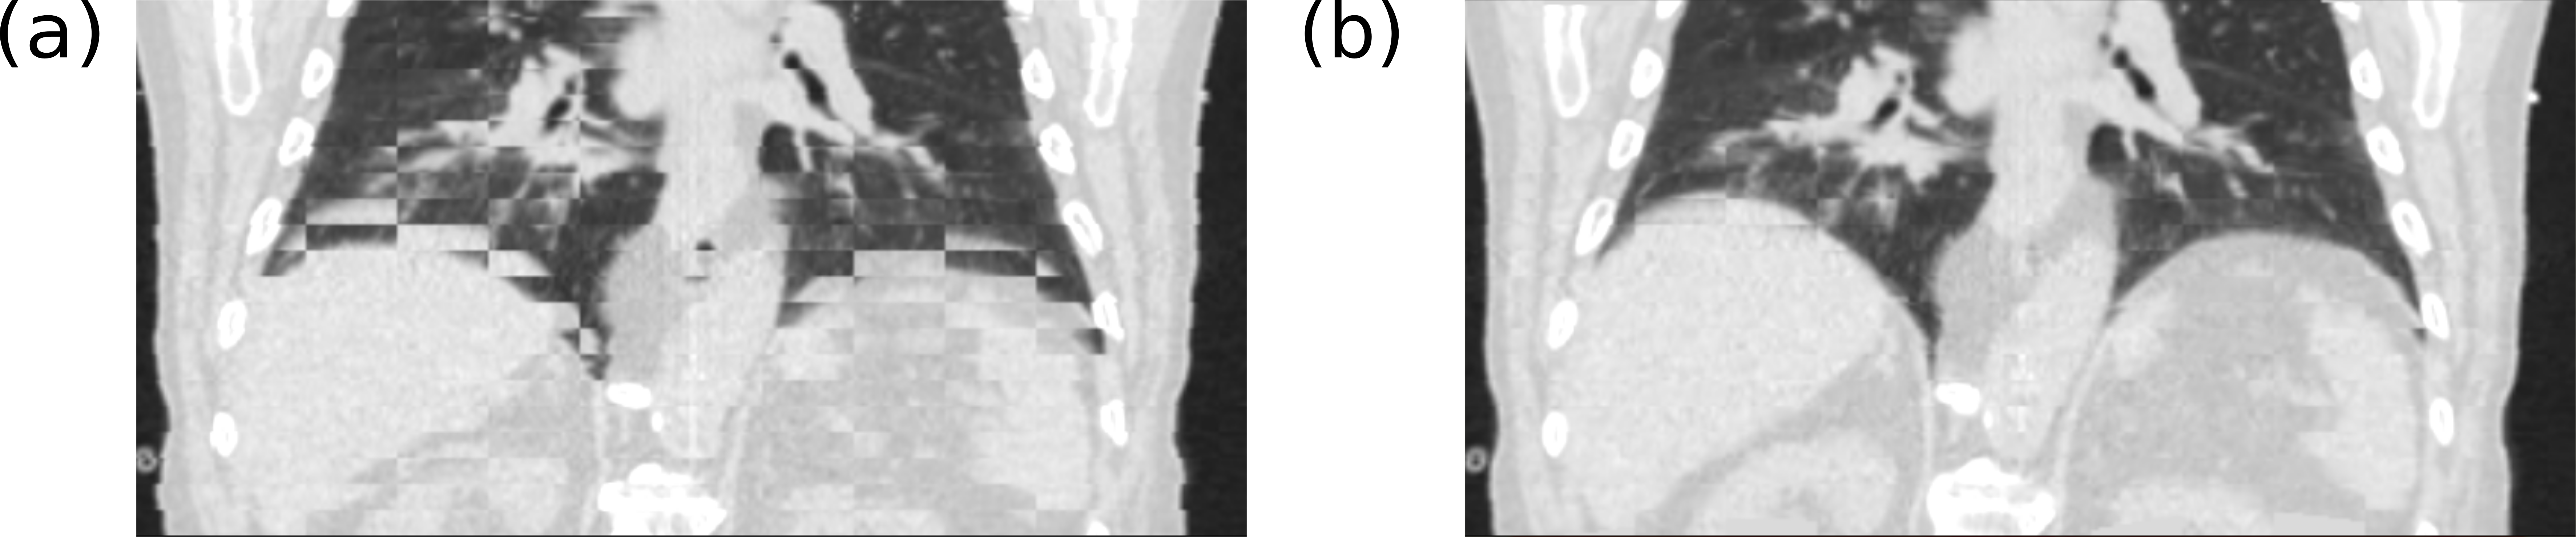
\includegraphics[width=0.9\textwidth]{./Vmm/Images/checkerboard.png}
		\caption{An example of a checkerboard image. It consists of tiles alternating between two images. Tiles in image (a) alternate between scans before registration and in image (b) after registration.}
		\label{checkerboard}
	\end{center}
\end{figure}

\subsubsection{Movie}

Medical images are usually quite large - a typical CT image consist of $512 \times 512 \times 100$ pixels, which makes inspecting image checks (inverse color, checkerboard, absolute difference) a time-consuming task. 
The movie feature allows a smoother display of different image slices. 
The user selects which view to inspect (axial, sagital or coronal) and presses start. Selected views then start scrolling from the first to the last slice of selected view. It allows user to focus on registration details, rather than scrolling through slices.



\subsubsection{Flicker}

While it is possible to display two images side by side in Slicer, it can sometimes be hard to see fine differences between the two images. Flicker alternates between reference and warped image on a single display at a 0.5 s rate. It allows
a quick inspection of differences between two images in their original form.

Movie and flicker (explained in the next section) do not offer any specific registration checks, but improve the process of DIRQA.

\subsubsection{Quantitative tests}

It can be hard to visually inspect all the DIR results, especially in a 4D-CT registration. Therefore a series of tests were developed that give a quantitative assessment of DIR quality.

\subsubsection{Absolute difference}

To stress the difference between reference and warped image an absolute difference between voxel values is calculated and displayed. 
A new image is generated with voxels populated as the absolute difference between reference and warped image voxel values, as shown in Fig.~\ref{absDiff}.
Furthermore, statistical values of absolute differences are calculated (mean, standard deviation, minimum and maximum) 
for a quantitative assessment of the registration quality (in the ideal case all values would be 0).

Three absolute differences can be calculated: between reference and moving image, called default absolute difference; between true warped and reference image, called true absolute difference; between inverse and moving image, called
inverse absolute difference. Usually, registration works on minimizing the absolute difference (mean square error metric), so it is a direct indicator
of registration success.

To save computational time or to focus on a specific region, the absolute difference can also be calculated just on a specific ROI (if used as an input). Usually the patient body is selected as ROI, without air and couch.


\begin{figure}[H]
	\begin{center}		
		\includegraphics[width=0.9\textwidth]{./Vmm/Images/abs.png}
		\caption{An absolute difference image before (a) and after registration (b). The mean absolute difference before registration (default absolute difference) is 62 HU and 31 HU after registration (true absolute difference).}
		\label{absDiff}
	\end{center}
\end{figure}


\subsubsection{Landmark distances}

Distances between landmarks before and after registration are often used to determine the spatial accuracy of registration \cite{Castillo2009}. 
Landmarks can either be a specific feature in the patient anatomy or an external marker. The position of landmarks in the warped image would ideally 
be at the same position as in the reference image. The module measures the Euclidean norm between the landmark positions in reference and warped image.

The user has to manually select landmarks in reference and moving or also in the warped image. For landmarks based on the patient anatomy, a selection from physician is required. 
Landmarks from the moving image can then be automatically transformed to the warped image using the registration vector field. An example is shown in Fig.~\ref{landmark}.

\begin{figure}[H]
\begin{center}
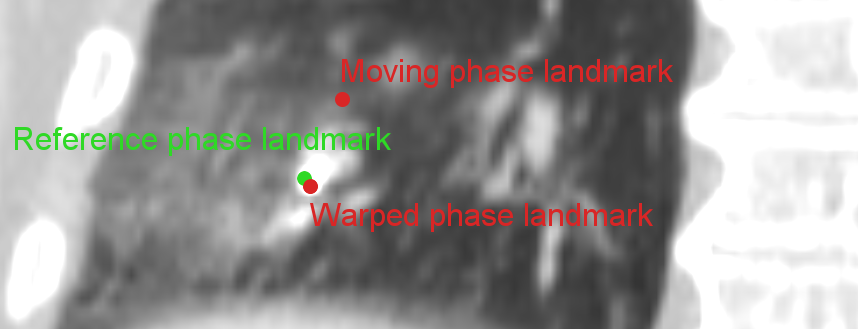
\includegraphics[width=0.9\textwidth]{./Vmm/Images/landmark.png}
\caption{A display of landmarks in three phases - reference, moving and warped phase. The distance before registration (between reference and moving landmark) is 22 mm and after registration
(between reference and warped landmark) is 2 mm.}
\label{landmark}
\end{center}
\end{figure}

\newpage
\subsubsection{Jacobian determinant}
\label{Jacobian}

The Jacobian determinant or Jacobian ($J$) of the vector field $u$ is calculated as:



\begin{equation}
J = \begin{vmatrix} 
\frac{\partial u_x}{\partial x} & \frac{\partial u_x}{\partial y} & \frac{\partial u_x}{\partial z} \\
\frac{\partial u_y}{\partial x} & \frac{\partial u_y}{\partial y} & \frac{\partial u_y}{\partial z} \\
\frac{\partial u_z}{\partial x} & \frac{\partial u_z}{\partial y} & \frac{\partial u_z}{\partial z} \\
\end{vmatrix}
\end{equation}

The Jacobian is used to validate the physical behavior of the registration \cite{Leow2007}. 
The Jacobian of a vector field should be positive, since negative Jacobian values correspond to organ folding, 
which is physically unrealistic for patient anatomy \cite{ Rey2002, Chen2008}. 
Expansions and contractions around a point are indicated by Jacobian values greater or lower than 1, respectively.

The DIRQA module calculates and displays the Jacobian of the vector field, as shown in Fig.~\ref{JacobianImage}.
Statistical values of the Jacobian are also calculated. Similar to the absolute difference, the Jacobian can be calculated inside a ROI rather than on the whole image.

\begin{figure}[H]
	\begin{center}		
		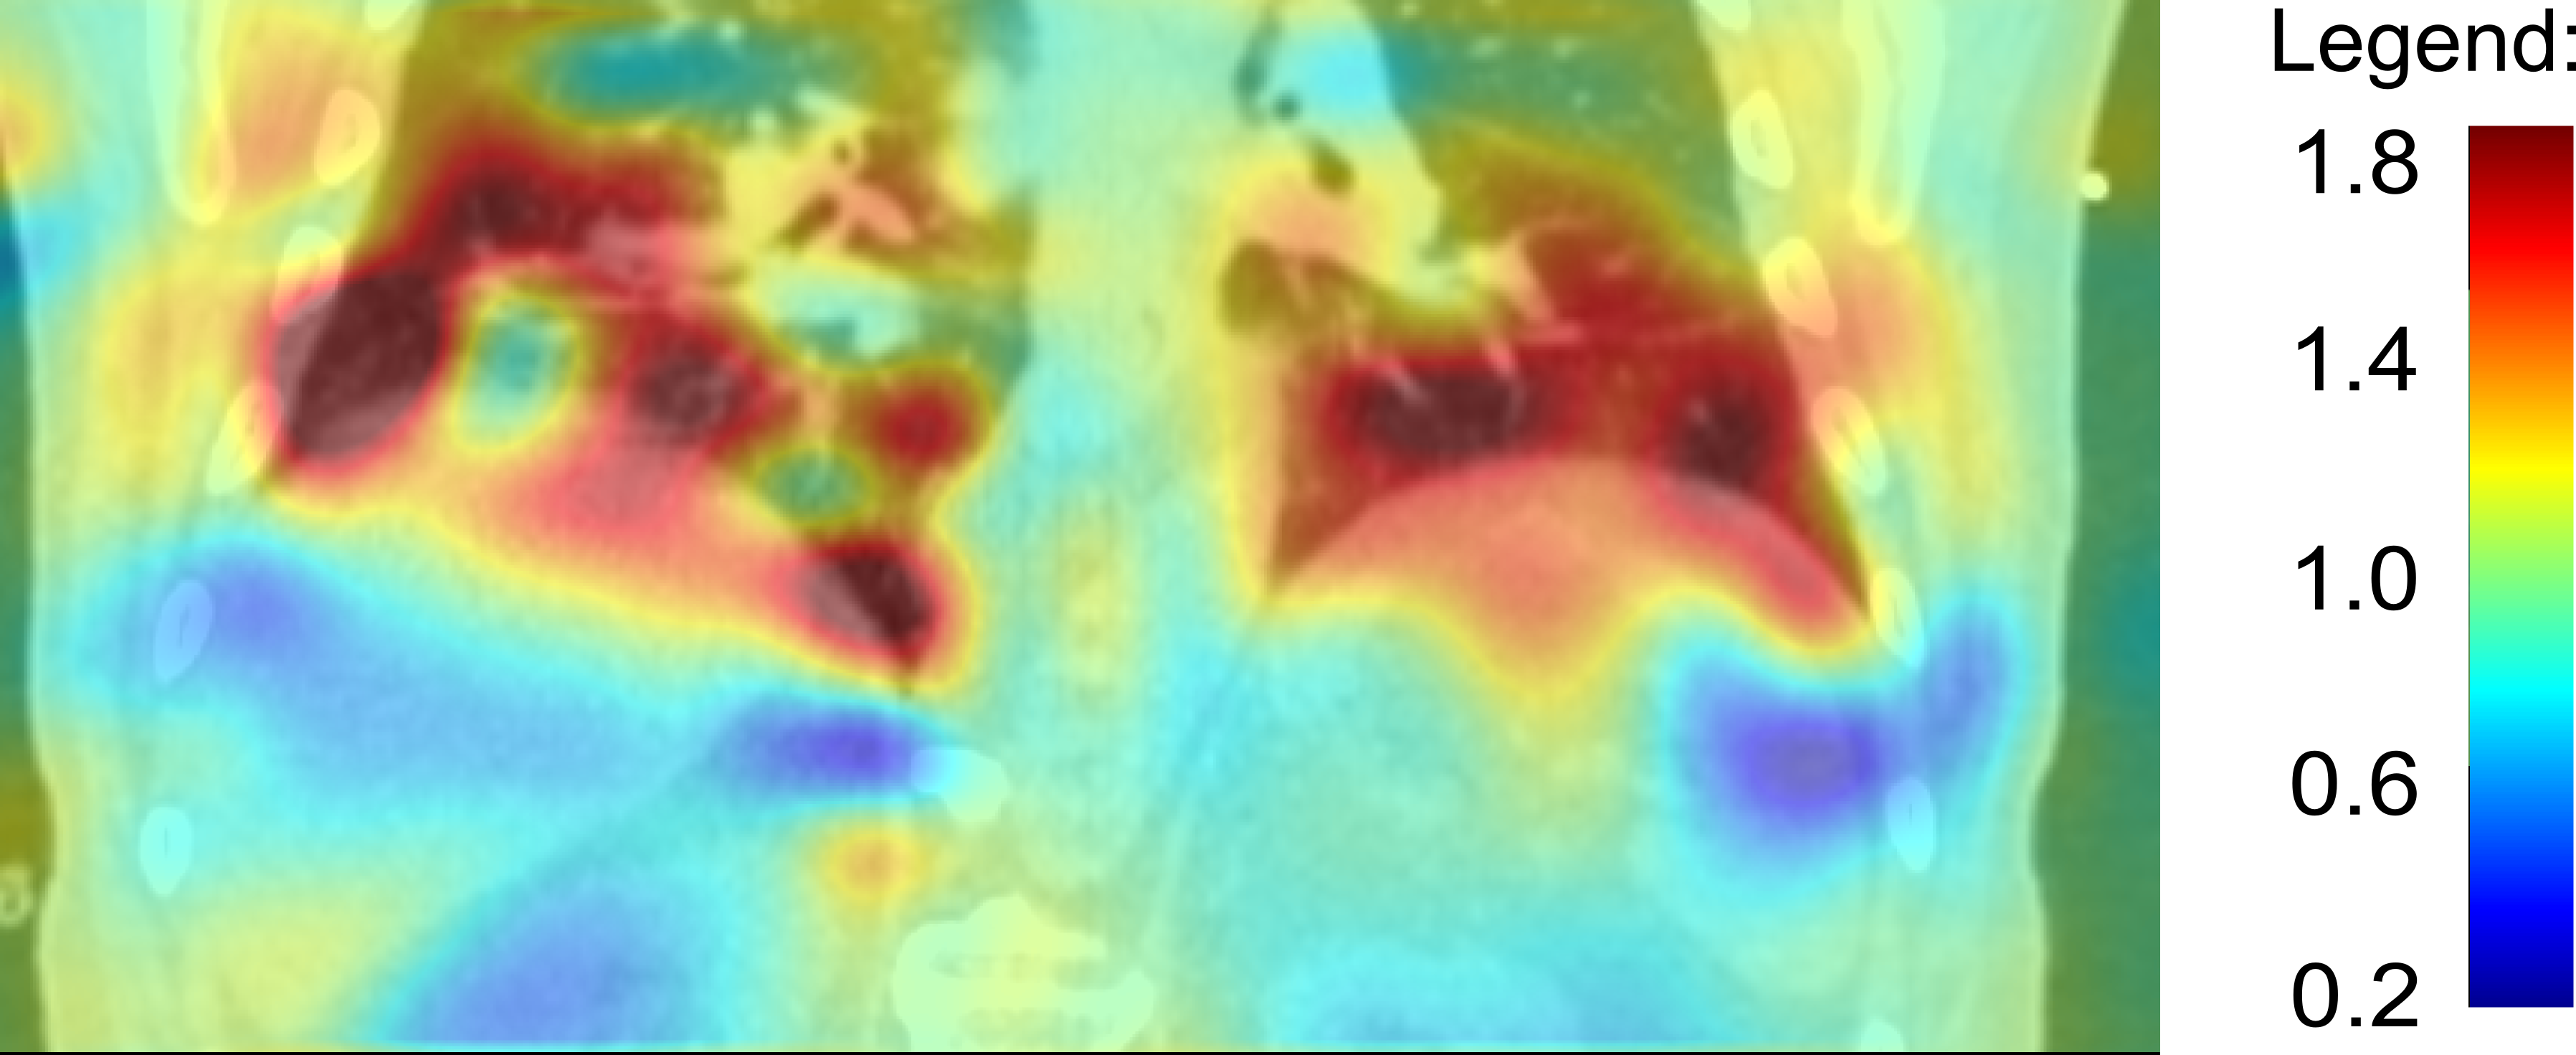
\includegraphics[width=0.8\textwidth]{./Vmm/Images/jacobian.png}
		\caption{An image of the Jacobian values overlayed on a CT scan. The average value of the displayed Jacobian is 0.98 with 0.09 standard deviation.}
		\label{JacobianImage}
	\end{center}
\end{figure}

\subsubsection{Inverse Consistency Error}
\label{ICE}

The inverse consistency error (ICE) is consistently used in literature as one of the main vector field checks \cite{Christensen2001, Bender2009}. The principle is as follows. 
Suppose we have two vector fields: $u_{AB}$ obtained from registration of image $A$ to $B$ and $u_{BA}$ from registration of image $B$ to $A$. The two registrations
are performed separately. In an ideal scenario, $u_{AB}$ would be a direct inverse of $u_{BA}$. However, DIR algorithms do not yield perfectly inverse consistent vector fields. Therefore, the differences between true and inverse vector fields have to be examined.


To check for ICE, an algorithm was created that first transforms a point $x$ in image $A$, using $u_{AB}$. The newly obtained point $x'$ is then transformed with the inverse vector
field, $u_{BA}$ which yields $x''$. The ICE is defined as Euclidean norm between $x$ and $x''$:

\begin{equation}
\label{eq:ice}
ICE = |x - x''| = |x - u_{BA}(x')| = |x - u_{BA}(u_{AB}(x))|
\end{equation}

Points $x'$ and $x''$ can have an arbitrary position in space, while vector fields $u_{AB}$ and $u_{BA}$ are positioned on a grid. To apply the transformation $u_{BA}(x')$, $x'$ is interpolated on a $u_{BA}$ grid. A tri-linear interpolation is used in this module.

As for the Jacobian, ICE image is calculated and displayed, along with statistical values and ROI feature. An example is shown in Fig.~\ref{inv}.




\begin{figure}[H]
\begin{center}
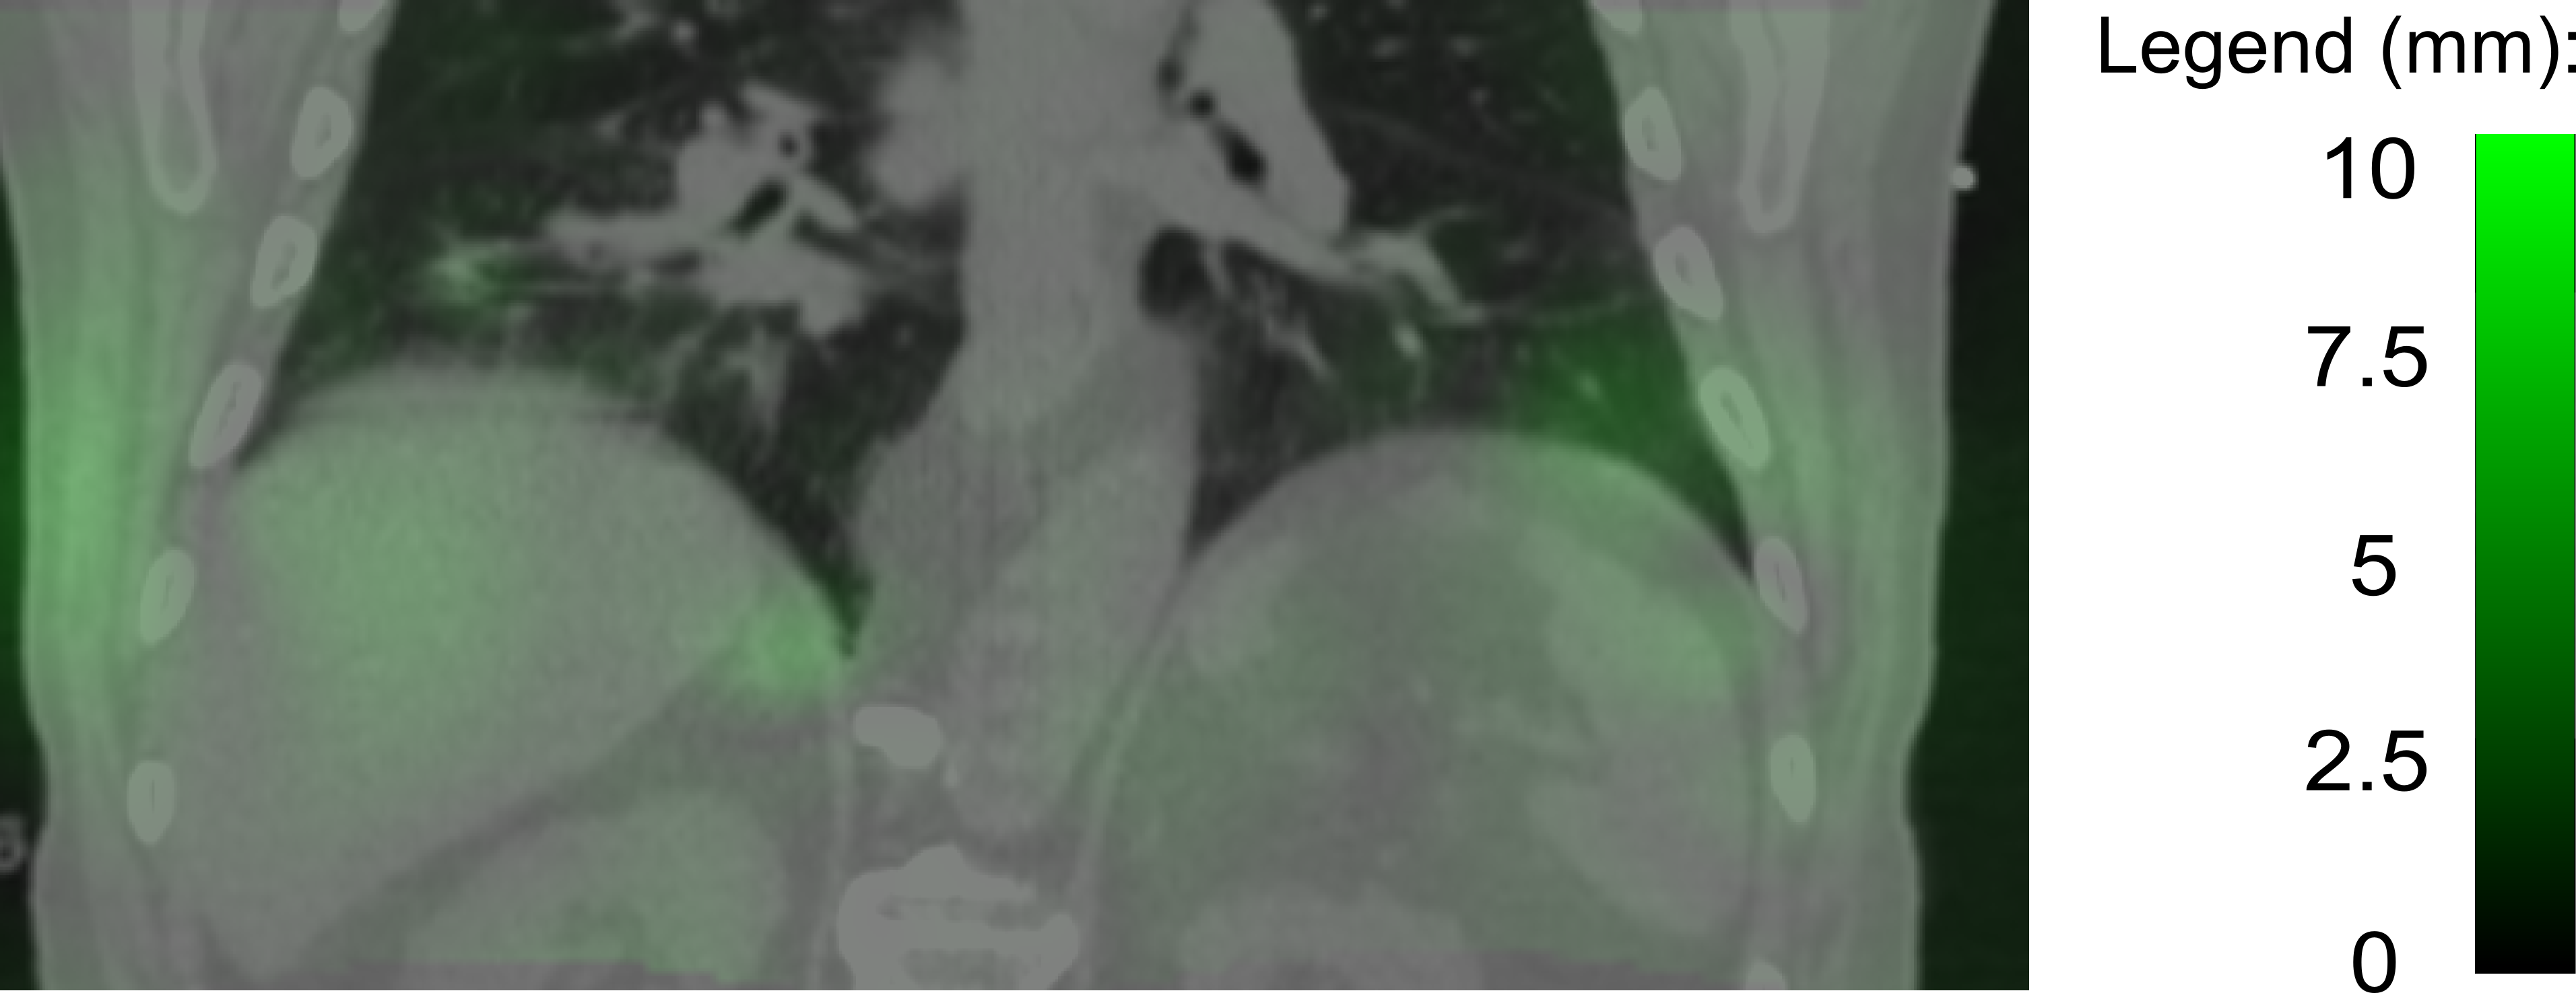
\includegraphics[width=0.8\textwidth]{./Vmm/Images/inv.png}
\caption{An image of the inverse consistency error (ICE) overlayed with CT scan. The average value of displayed ICE is 1.0 mm with 0.8 mm standard deviation.}
\label{inv}
\end{center}
\end{figure}


% \subsubsection{Output file}
% 
% With all different features to validate DIR it can be time consuming to go through them all. A special option was created to automatically go through all different validation steps. Furthermore it can also run through different phases, if there are more phases (i.e. in 4D-CT). All produced data from DIR validation is stored on disk and can be reexamined by user upon request. Furthermore, images are created and data is summed up and displayed in a separate file. Users can then preview file for first validation of DIR and then open necessary files, if required.

% \subsection{Contour visualization}
% \label{Contour}
% 
% TRiP4D (see Section \textbf{REF}) introduced volume datasets for contour representation \cite{Richter2012}. It enabled necessary tasks for 4D calculations, such as the storing contour in different 4D states, contour propagation, etc. However, there was a lack of a proper visualization tool. In order to provide a contour visualization tool, a Slicer module was created. 
% 
% Contours are saved as volumetric boolean masks. A single bit per ROI contour representation marks each voxel inside volume dataset \cite{Richter2012}. To properly display contour, first a whole volume dataset was imported in Slicer. User selects which motion state he would like to inspect. The corresponding bit is then selected on the imported volume dataset. Lastly the contour is converted into 3D model shape. 
% 
% \subsection{Motion estimation and ITV creation}
% 
% ITV is often created by an eye investigation of all 4D-CT phases, where the extent of motion is estimated. Automatic creation of ITV is scarce in commercial system, since it requires DIR on all 4D-CT phases. A Slicer module was created to assist with the motion estimation and automatic ITV creation using DIR. 
% 
% Module is able to estimate and display motion of a user selected contour in three axis (left-right, anterior-posterior, superior-inferior) based on DIR vector fields. Module also performs DIR on 4D-CT with patient hierarchy, if it has not been done yet.
% 
% Beside motion estimation, module can also propagate selected contour (usually CTV) and propagate it to all 4D-CT and make a convolution of all propagated contours, resulting in automatically generated ITV.
% 
% \subsubsection{Generation of mid-position phase}
% 
% Most commercial software calculates treatment plan on a single 3D CT scan, using 4D-CT only for motion estimation. To incorporate patient-specific motion information, a 3D CT scan was created from 4D-CT in the time averaged position, also known as mid-position scan (midP scan) \cite{Wolthaus2008}. With midP scan commercial software can still be used. Additionally, it also enabled smaller error margins for PTV generation and midP scan has less noise as individual 4D-CT scans, because it uses more data. 
% 
% Construction of a midP begins with registration of whole 4D-CT. The resulting vector fields from reference position to 4D-CT phases are then averaged to obtain mean vector field, see Fig.~\ref{midPgeneration}. Afterwards, for each vector field the mean vector field was subtracted, yielding a set of mean-corrected vector fields pointing from mean position to corresponding 4D-CT phase. The mean-corrected vector fields were finally inverted and applied to each 4D-CT phase, resulting in each phase being in the same, time-averaged position. In the end the set of transformed 4D-CT phase was averaged to obtain midP scan.
% 
% \begin{figure}[H]
% \begin{center}
% 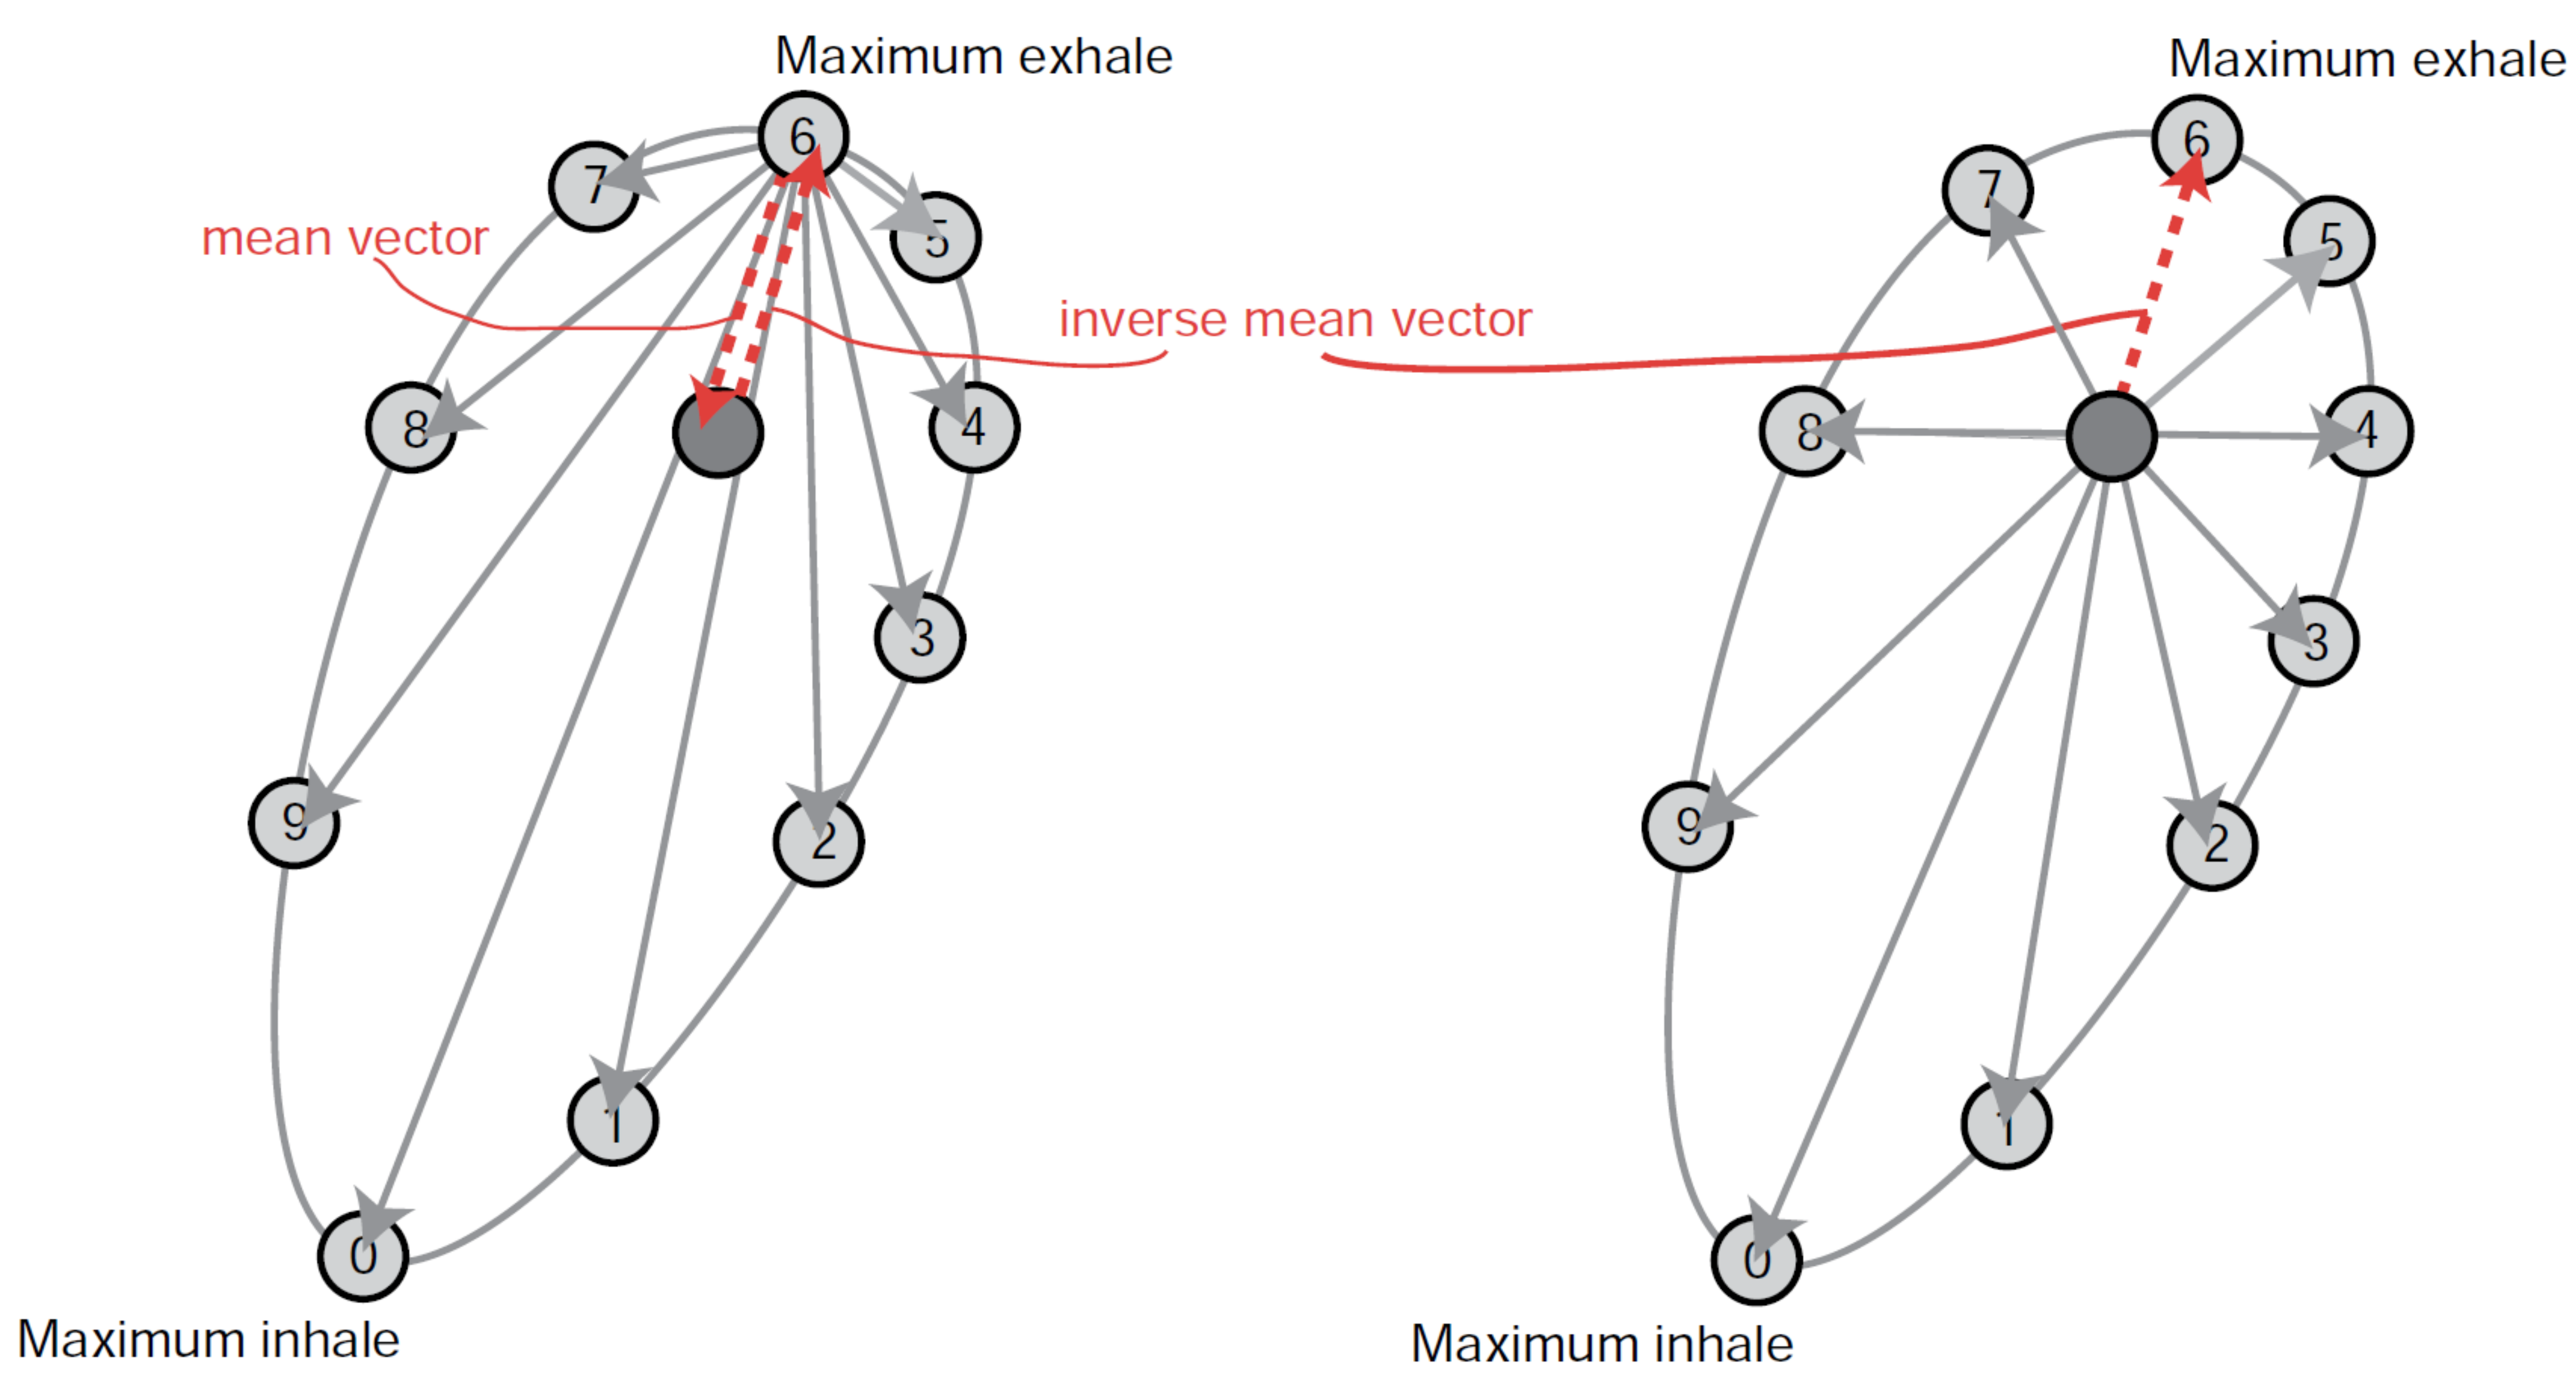
\includegraphics[width=0.9\textwidth]{./Vmm/Images/midPgeneration.png}
% \caption{Computation of the midP scan. All vectors have the same starting point (reference phase, maximum exhale in the this example), therefore they can be averaged, resulting in the mean vector.
% 	Next vectors from mean position to 4D-CT phases have to be computed, which is achieved by subtracting original vectors and mean vector. Figure taken from \cite{Wolthaus2008}}
% \label{midPgeneration}
% \end{center}
% \end{figure}


\newpage
\section{Verification}
\label{Verification}

Several tools to perform DIR and DIRQA were created. To prove their functionalities, we have tested them on two sets of an actual clinical data. 
First were the lung 4D-CT patient data from the Champalimaud Center for the Unknown, Lisbon (Portugal). The 4D-CTs were used in the treatment planning study, presented in Chapters~\ref{PatStudy} and \ref{chapter:complex}. 
DIR resulting from 4D-CTs play an essential  will be used in contour propagation in order to estimate tumor motion. Additionally, DIR will be also used in 4D dose calculation.

The second set of data 
It is therefore necessary
and pig cardiac 4D-CT, that were part of an animal study \cite{Lehmann2015},
were included in a verification. All 4D-CTs were registered to the 4D-CT's reference data. Absolute difference, Jacobian and ICE were calculated for resulting 
DIR as part of a DIRQA.

\subsection{Registration of lung 4D-CT patient data}
\label{lungDIR}

Chapters \ref{PatStudy} and \ref{chapter:complex} present studies on simulating active scanning carbon ion treatment PT for non-small cell lung cancer patients. 
The effects of interplay can drastically change the dose distribution for PT and it is necessary to quantify the effects of motion with DIR and transfer results into a treatment 
planning software. We used a GSI's in-house treatment planning software, TRiP98 \cite{Kraemer2000a, Richter2013}. An automated procedure was required to perform DIR and DIRQA on a large number of patients. This was achieved with Slicer modules described in Section~\ref{Implementation}.

\subsubsection{Materials and Methods}

A time-resolved CT (4D-CT), consisting of 10 motion states (0 - 9) with 1 mm pixel and 1-2 mm slice spacing was acquired with either a Philips Brilliance BigBore 16-slice 
(Philips Healthcare, Eindhoven, Netherlands) or a Philips Gemini PET-CT 16-slice scanner. 
State 0 and 5 correspond to the end-inhale and end-exhale breathing state, respectively. State 0 was chosen as a reference state. 23 4D-CTs of lung cancer patients were used in this study.

True and inverse DIR were computed for each patient between each state and the reference state. Each 4D-CT required 18 DIRs, leading to 414 DIRs in total.

The B-Spline Plastimatch module in Slicer was used for DIR (see Section~\ref{RegistrationImplement}). DIRs were done in two stages with details given in Table~\ref{tab:stages}. 

\begin{table}[H]
  \centering
%   \footnotesize
  \caption{Parameters used for B-Spline Plastimatch DIR. A mean squared error metric was used. Details for each parameter can be found in \cite{Plastimatch}.}
  \begin{tabular}{c|c|c}
      Parameter & Stage 1 & Stage 2 \\
      \hline
      Resolution & 4,4,2 & 1,1,1 \\
      Grid size & 50 & 15 \\
      Regularization lambda & 0.005 & 0.005 \\
      Iterations & 200 & 100 \\
    \hline\hline
  \end{tabular}
  \label{tab:stages}
\end{table}

\begin{figure}[H]
	\begin{center}		
		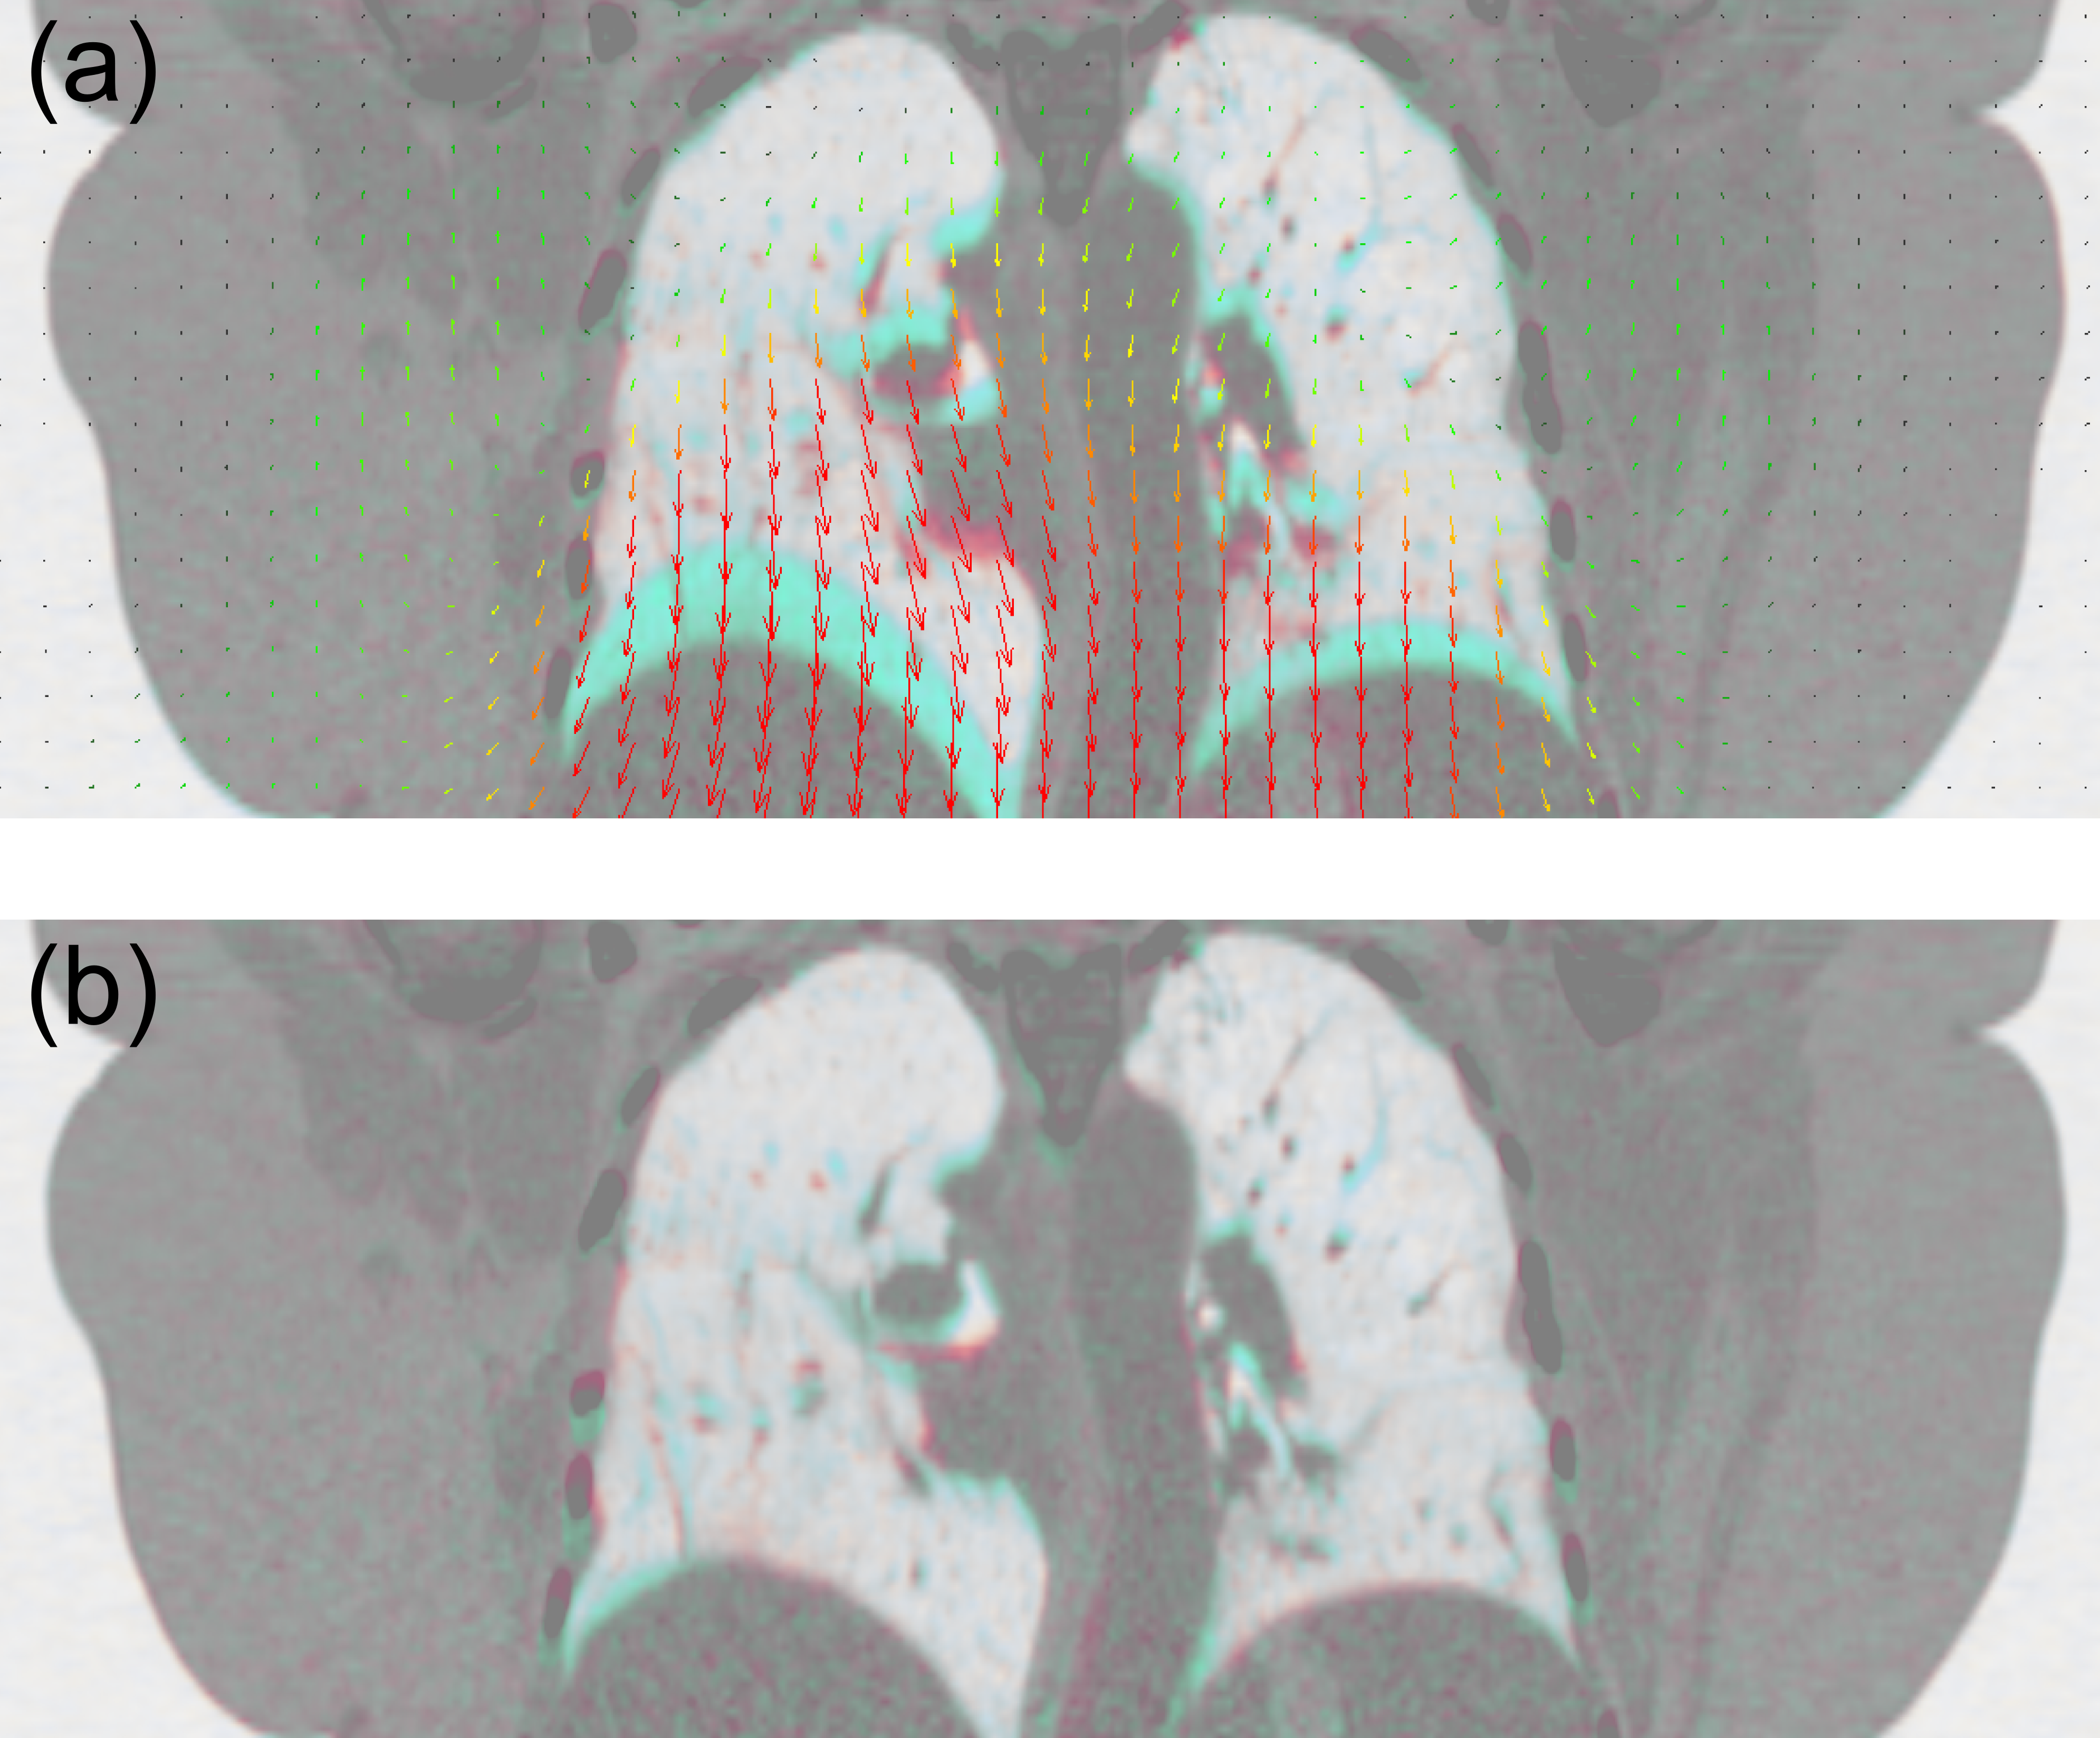
\includegraphics[width=0.6\textwidth]{./Vmm/Images/exampleReg.png}
		\caption{Inverse color overlay of two states before (a) and after (b) DIR. Vector field is displayed on image (a) as arrows.}
		\label{exampleReg_lung}
	\end{center}
\end{figure}

A box around the patient body was created with a Slicer feature. The box was then used as a ROI in calculation of absolute difference, Jacobian and ICE.

Default, true and inverse absolute difference were calculated. In total 621 absolute differences were calculated. All images were down-sampled by a factor of 2
before calculation to save computer time. Similarly, 414 vector fields were down-sampled by a factor of 2 before calculating Jacobian and ICE. Jacobian and ICE checks were calculated on all vector fields.
Additionally, each vector field magnitudes were analyzed for mean, standard deviation (STD) and maximum (max) values. Paired t-tests were performed to compare statistical values of true and inverse vector field magnitudes.
A p-value < 0.05 was considered significant. A Pearson's r coefficient was used to determine linear fit quality.


For each patient it took around 20 min for all 18 DIR and around 30 min for complete DIRQA on the 18 DIR. A Linux computer with 8 CPU and 32 GB RAM was used for DIR and DIRQA.

DIR was used in treatment planning, specifically in contour propagation and 4D dose calculation. The areas with poor DIR were investigated and distance between DIR errors 
and target contour was measured. If target was more than 5 cm away from DIR errors, DIR was not repeated.


\subsubsection{Results}

An example of DIR is displayed in Fig.~\ref{exampleReg_lung}. The statistical analysis of vector fields is shown in Table~\ref{tab:vectordata_lung}. There was no statistical
difference between true and inverse vector field magnitudes. The biggest contribution to vector field magnitude was from superior-inferior direction (around 50\%), followed by anterior-posterior direction (around 30\%)
by left-right direction (around 20\%).

\begin{table}[H]
  \centering
%   \footnotesize
  \caption{Data of vector magnitudes. Values are presented as mean (range).}
  \begin{tabular}{c|c|c}
  
       & True vector field (mm) & Inverse vector field (mm) \\
       \hline
       Mean & 0.38 (0.01 - 1.28) & 0.38 (0.01 - 1.3) \\ 
       STD & 0.95 (0.04 - 3.17) & 0.98 (0.04 - 3.55) \\ 
       Max & 9.67 (0.61 - 28.56) & 10.17 (0.56 - 37.11) \\
    \hline\hline
  \end{tabular}
  \label{tab:vectordata_lung}
\end{table}

True and inverse absolute difference dependence on default absolute difference is shown in Fig.~\ref{absDiff_lung}. It also shows default absolute difference distribution across 9 states. 

Distribution of true and inverse Jacobian and ICE data are displayed in Fig. \ref{jacobian_data}. 

True and inverse maximum and minimum Jacobian and maximum ICE values were plotted against maximum vector magnitudes and fitted with linear function. Results are shown in Fig.~\ref{maxvf}.


Linear fits used in Fig.~\ref{absDiff_lung} and ~\ref{maxvf} were statistically significant (p < 0.05).

All areas with poor DIR were further than 5 cm away from the target and no repetition of DIR was necessary.

\begin{figure}[H]
	\begin{center}		
		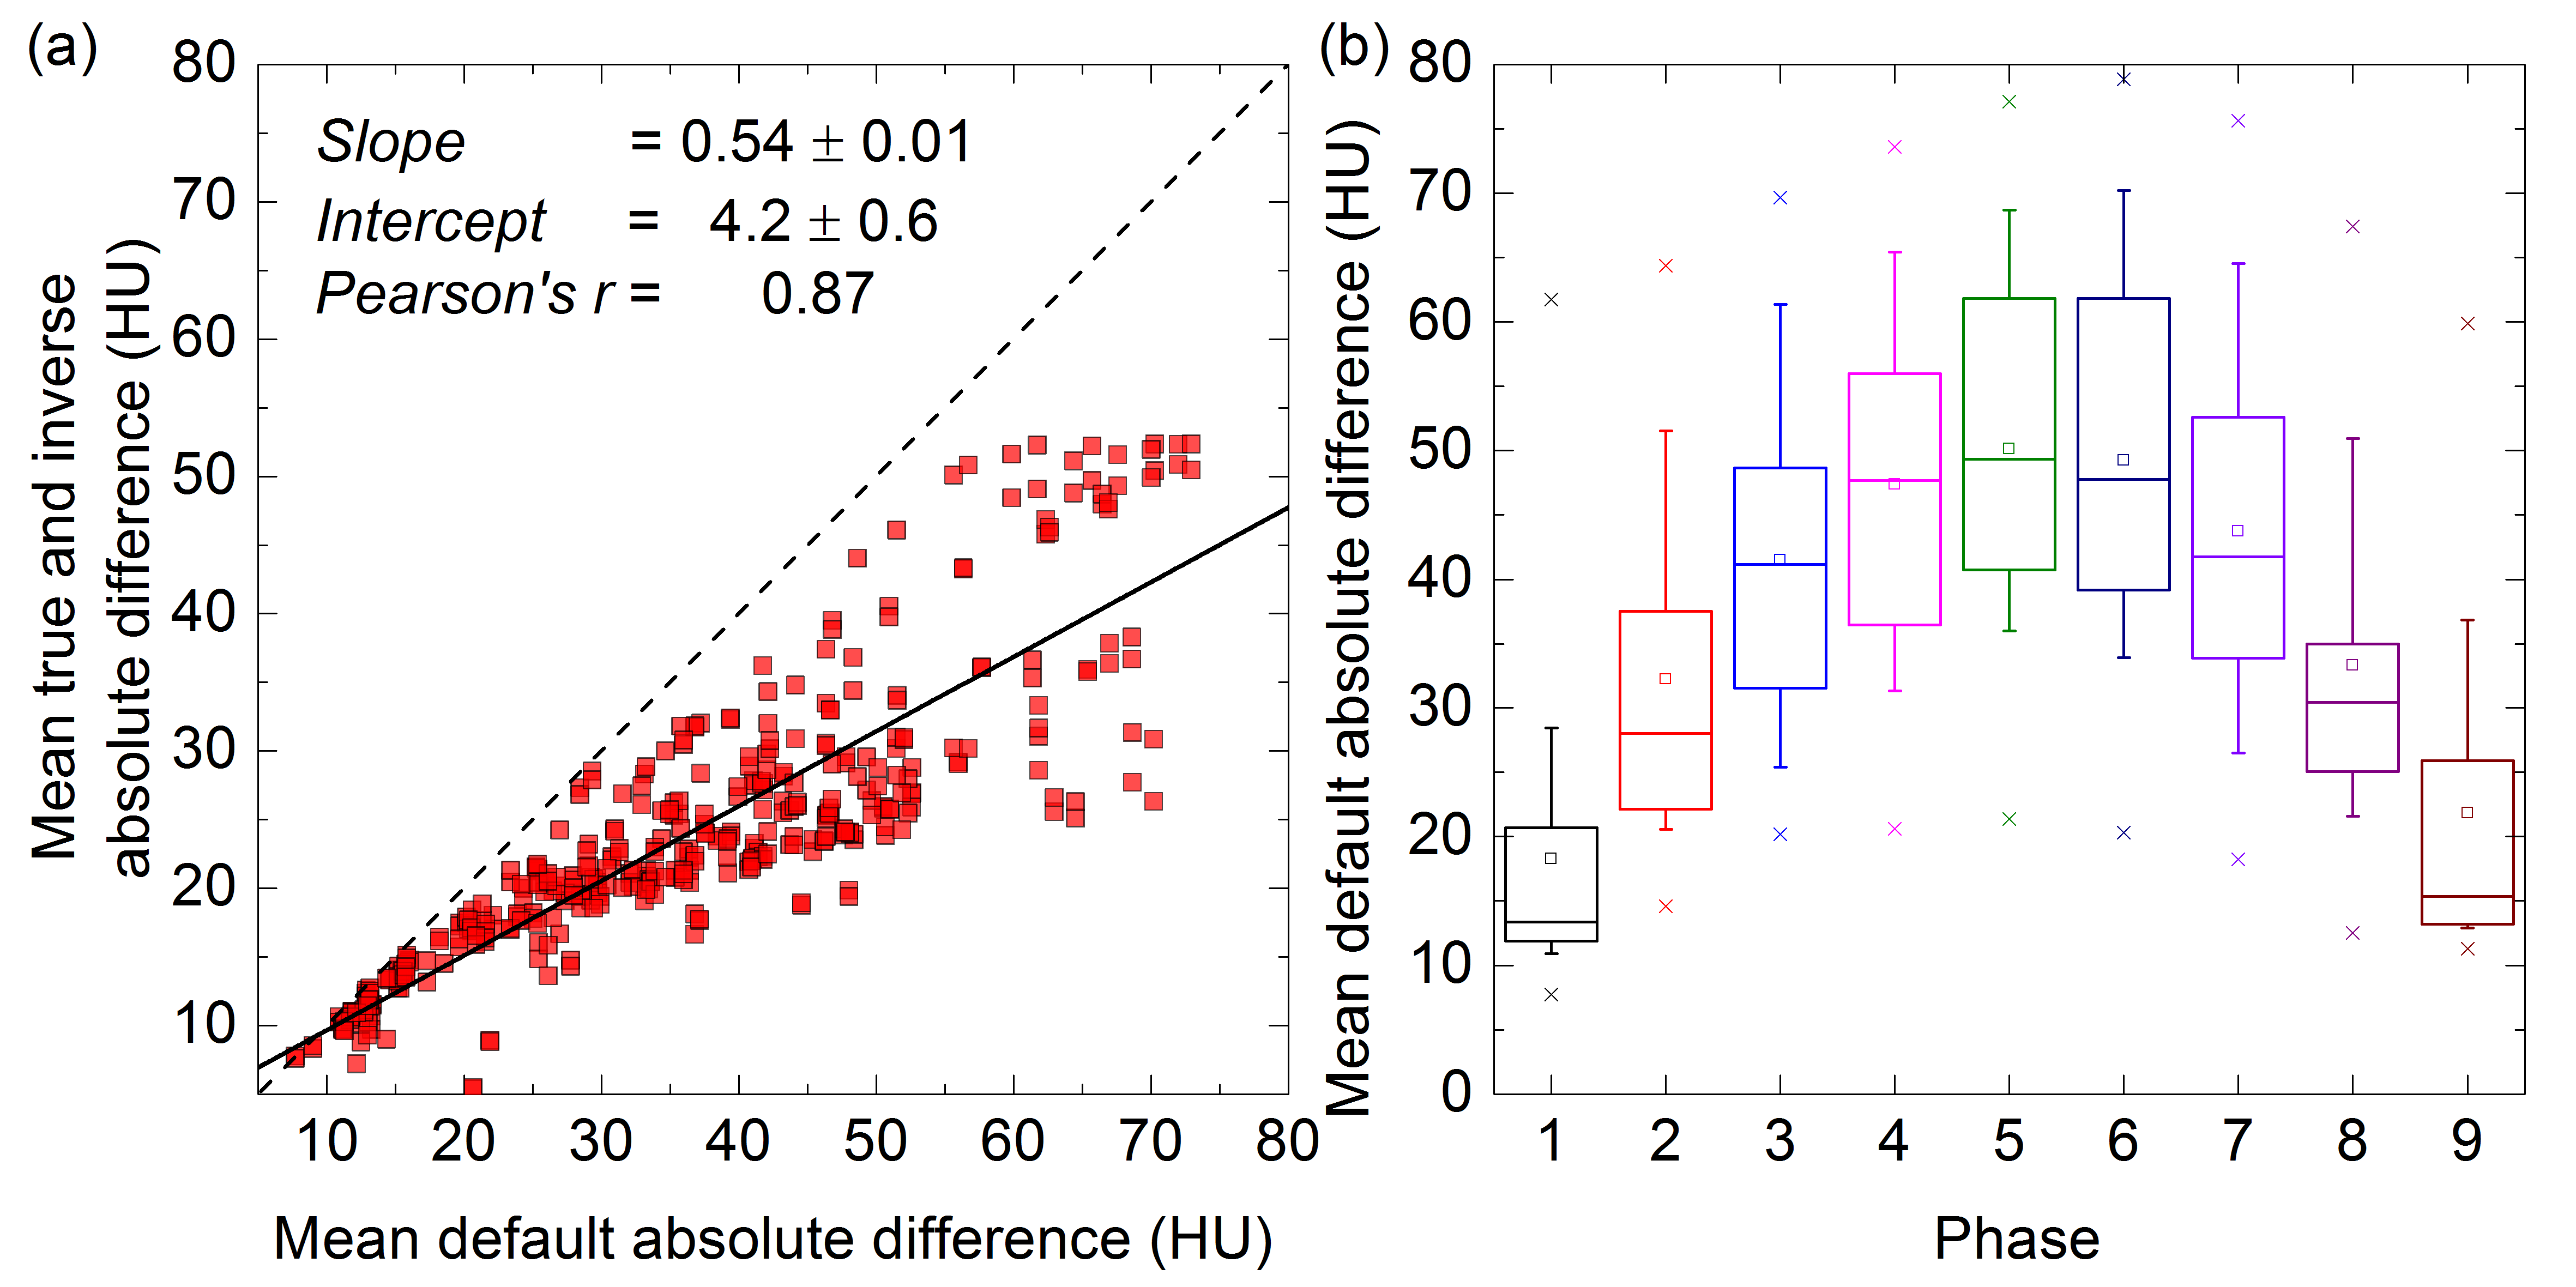
\includegraphics[width=0.7\textwidth]{./Vmm/Images/absDiff.png}
		\caption{(a) Mean true and inverse absolute difference plotted against mean default absolute difference. Solid line shows linear fit, with parameters
		written in corner. Dashed line shows $y(x)=x$. (b) Box plots of mean default absolute difference distribution across nine 4D-CT states. Boxes represent 25-75\%, whiskers 10-90\%
		of data, median is shown with a solid line, mean with squares and outliers with crosses.}
		\label{absDiff_lung}
	\end{center}
\end{figure}

\newpage

\begin{figure}[H]
	\begin{center}		
		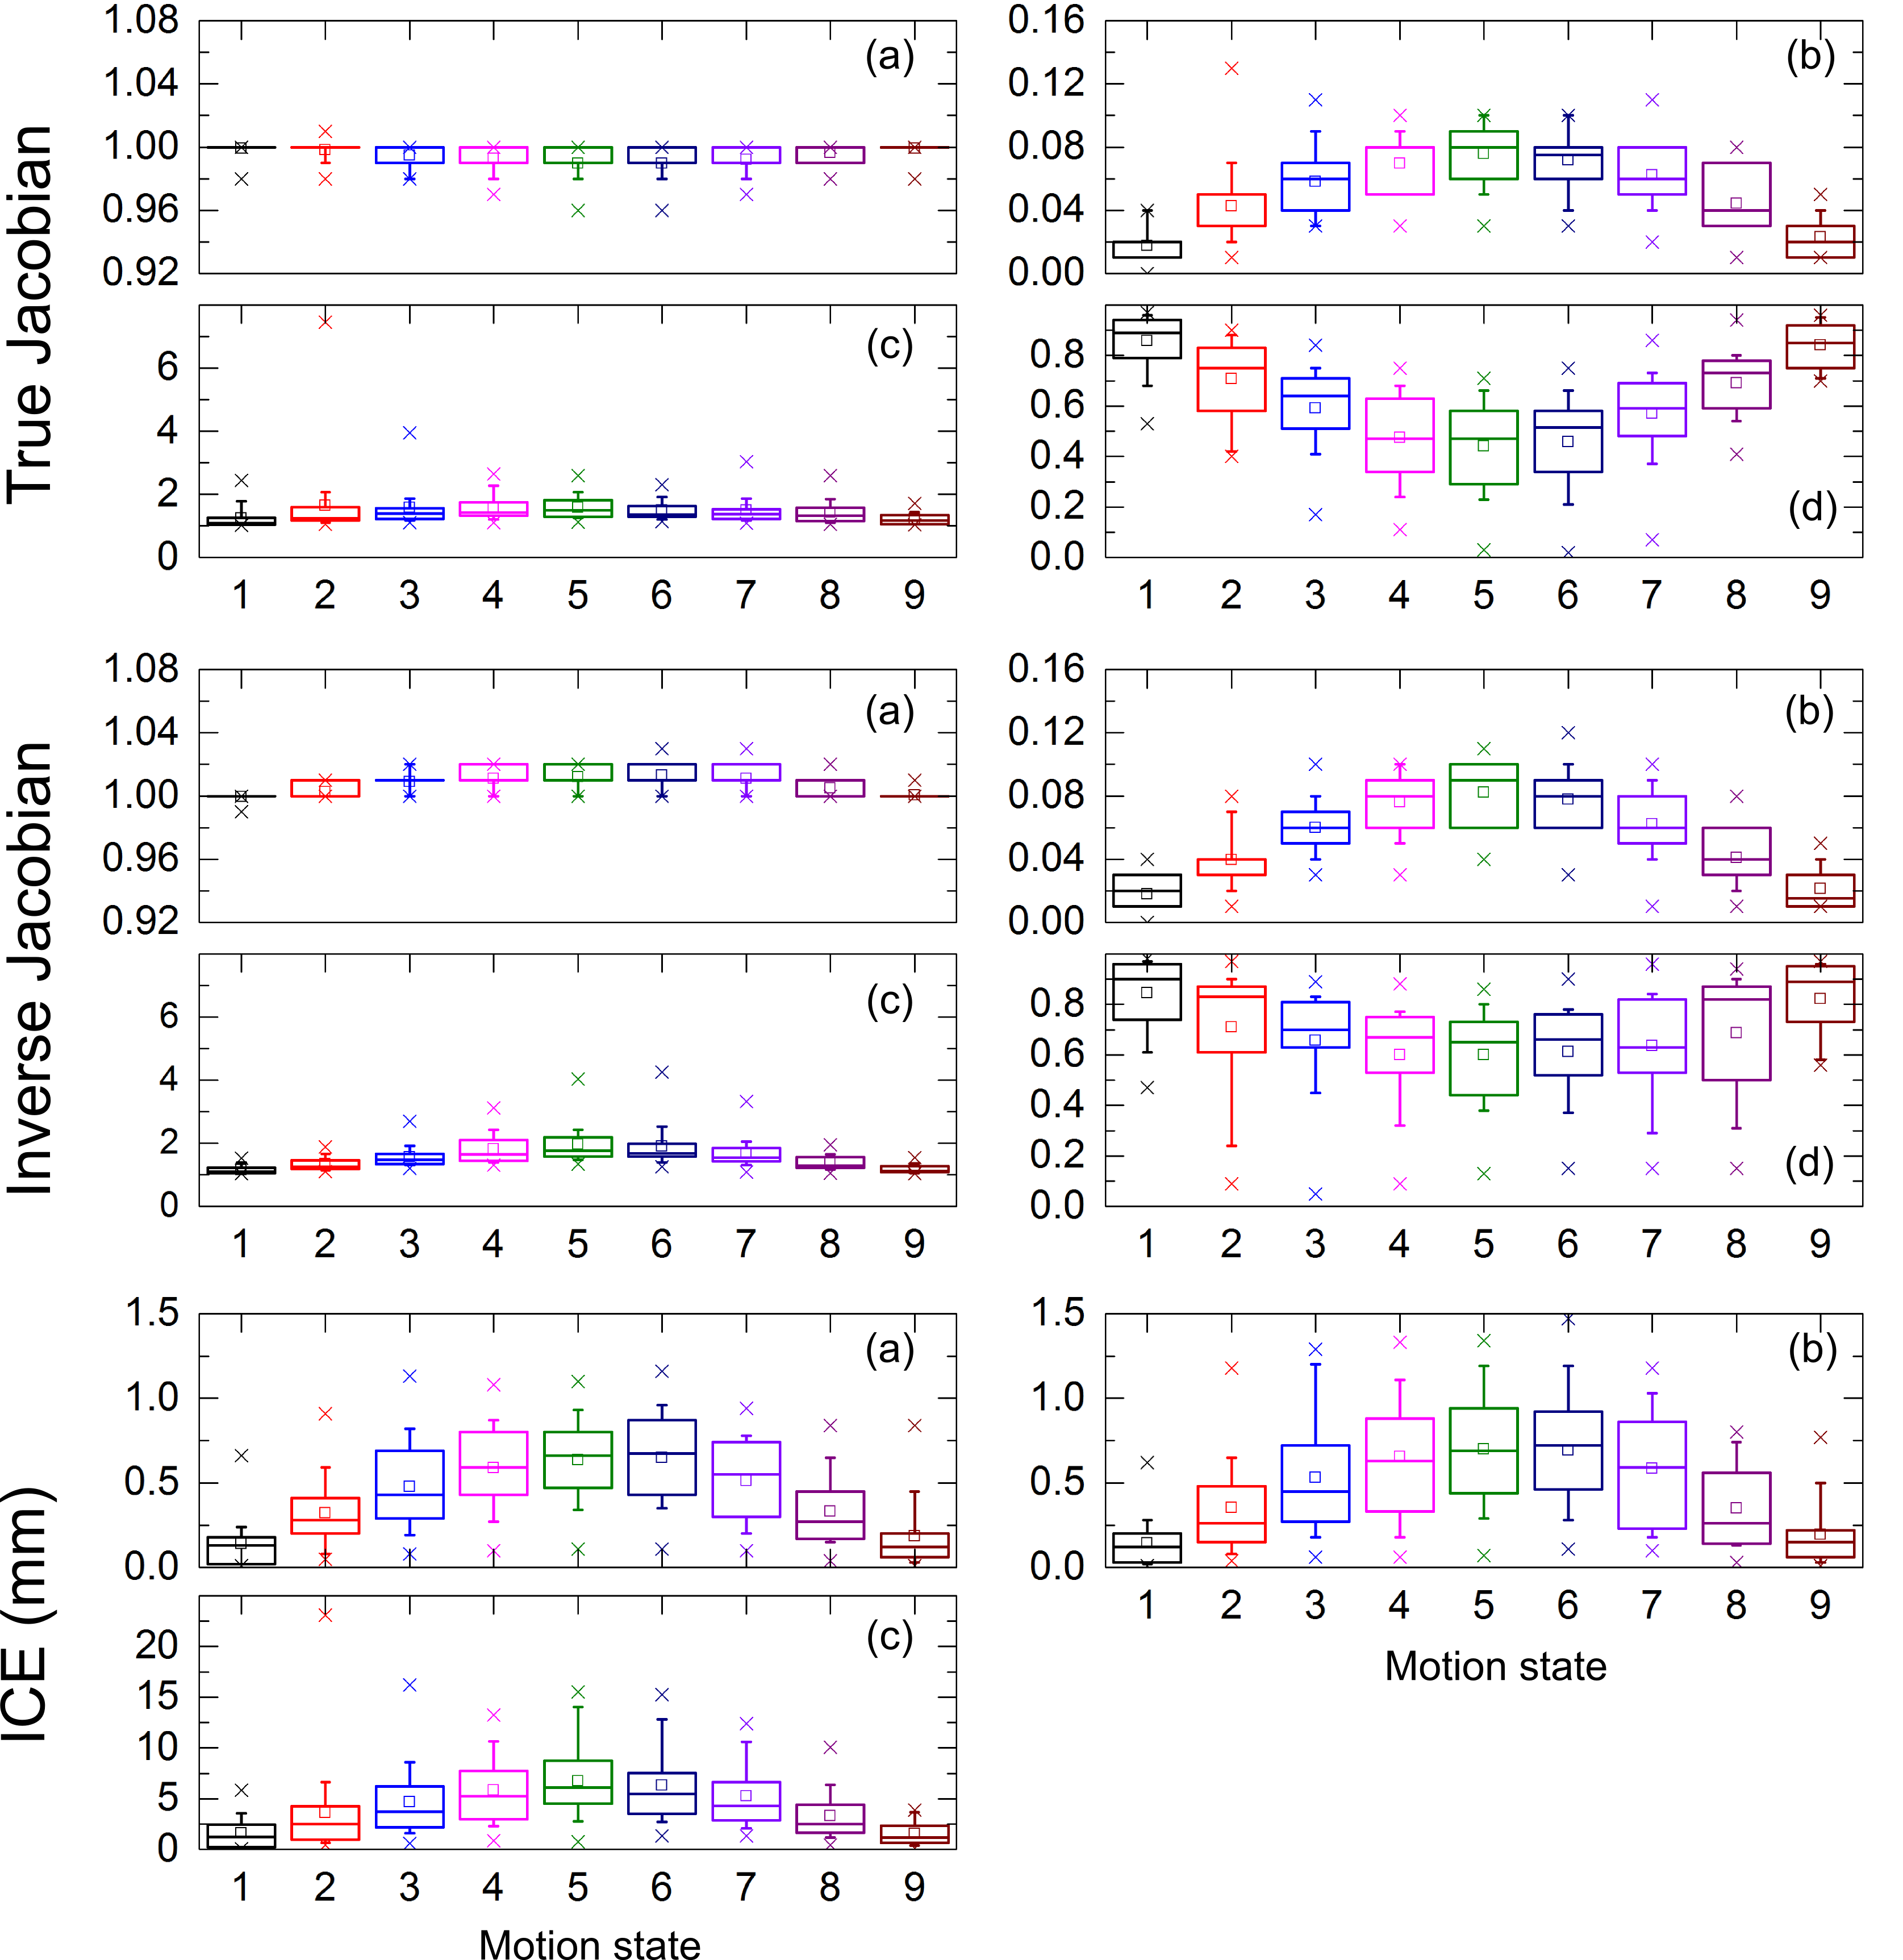
\includegraphics[width=0.9\textwidth]{./Vmm/Images/Jacobian_data.png}
		\caption{Data for true (top) and inverse (middle) Jacobian and ICE (bottom) for 9 4D-CT states (reference state 0 is excluded) for 23 lung cancer patients. Mean, STD, maximum and minimum are represented as (a), (b), (c) and (d), respectively.
		Minimum ICE is 0 throughout all states and patients. Boxes represent 25-75\%, whiskers 10-90\% of data, median is shown with a solid line, mean with squares and outliers with crosses.}
		\label{jacobian_data}
	\end{center}
\end{figure}

\newpage

% \begin{figure}[H]
% 	\begin{center}		
% 		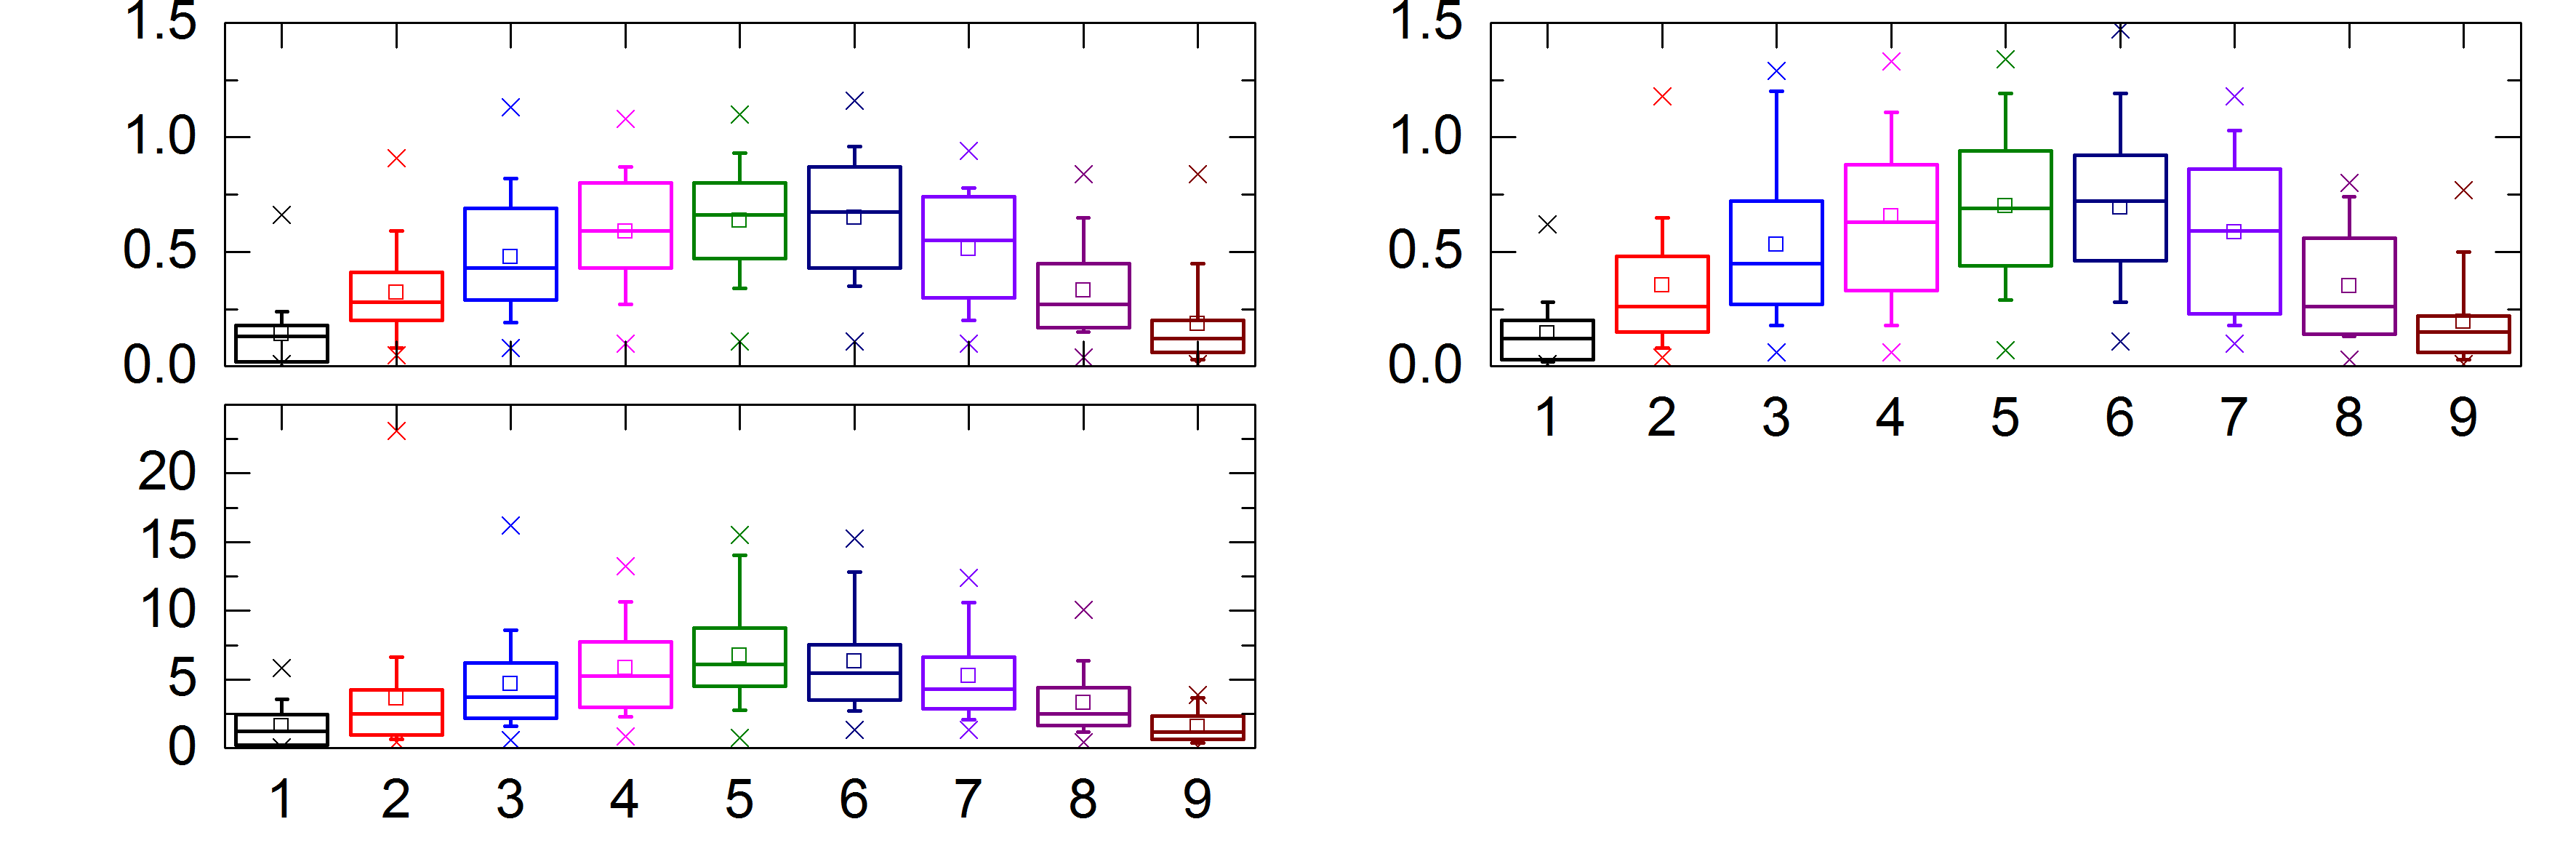
\includegraphics[width=0.9\textwidth]{./Vmm/Images/ICE.png}
% 		\caption{Data for ICE for 9 4D-CT states (reference state 0 is excluded) for 23 lung cancer patients. Mean, STD, maximum are represented as (a), (b) and (c), respectively. ICE Minimum is 0 throughout all states and patients.
% 		Boxes represent 25-75\%, whiskers 10-90\% of data, median is shown with a solid line, mean with squares and outliers with crosses.}
% 		\label{ice}
% 	\end{center}
% \end{figure}



% \begin{figure}[H]
% 	\begin{center}		
% 		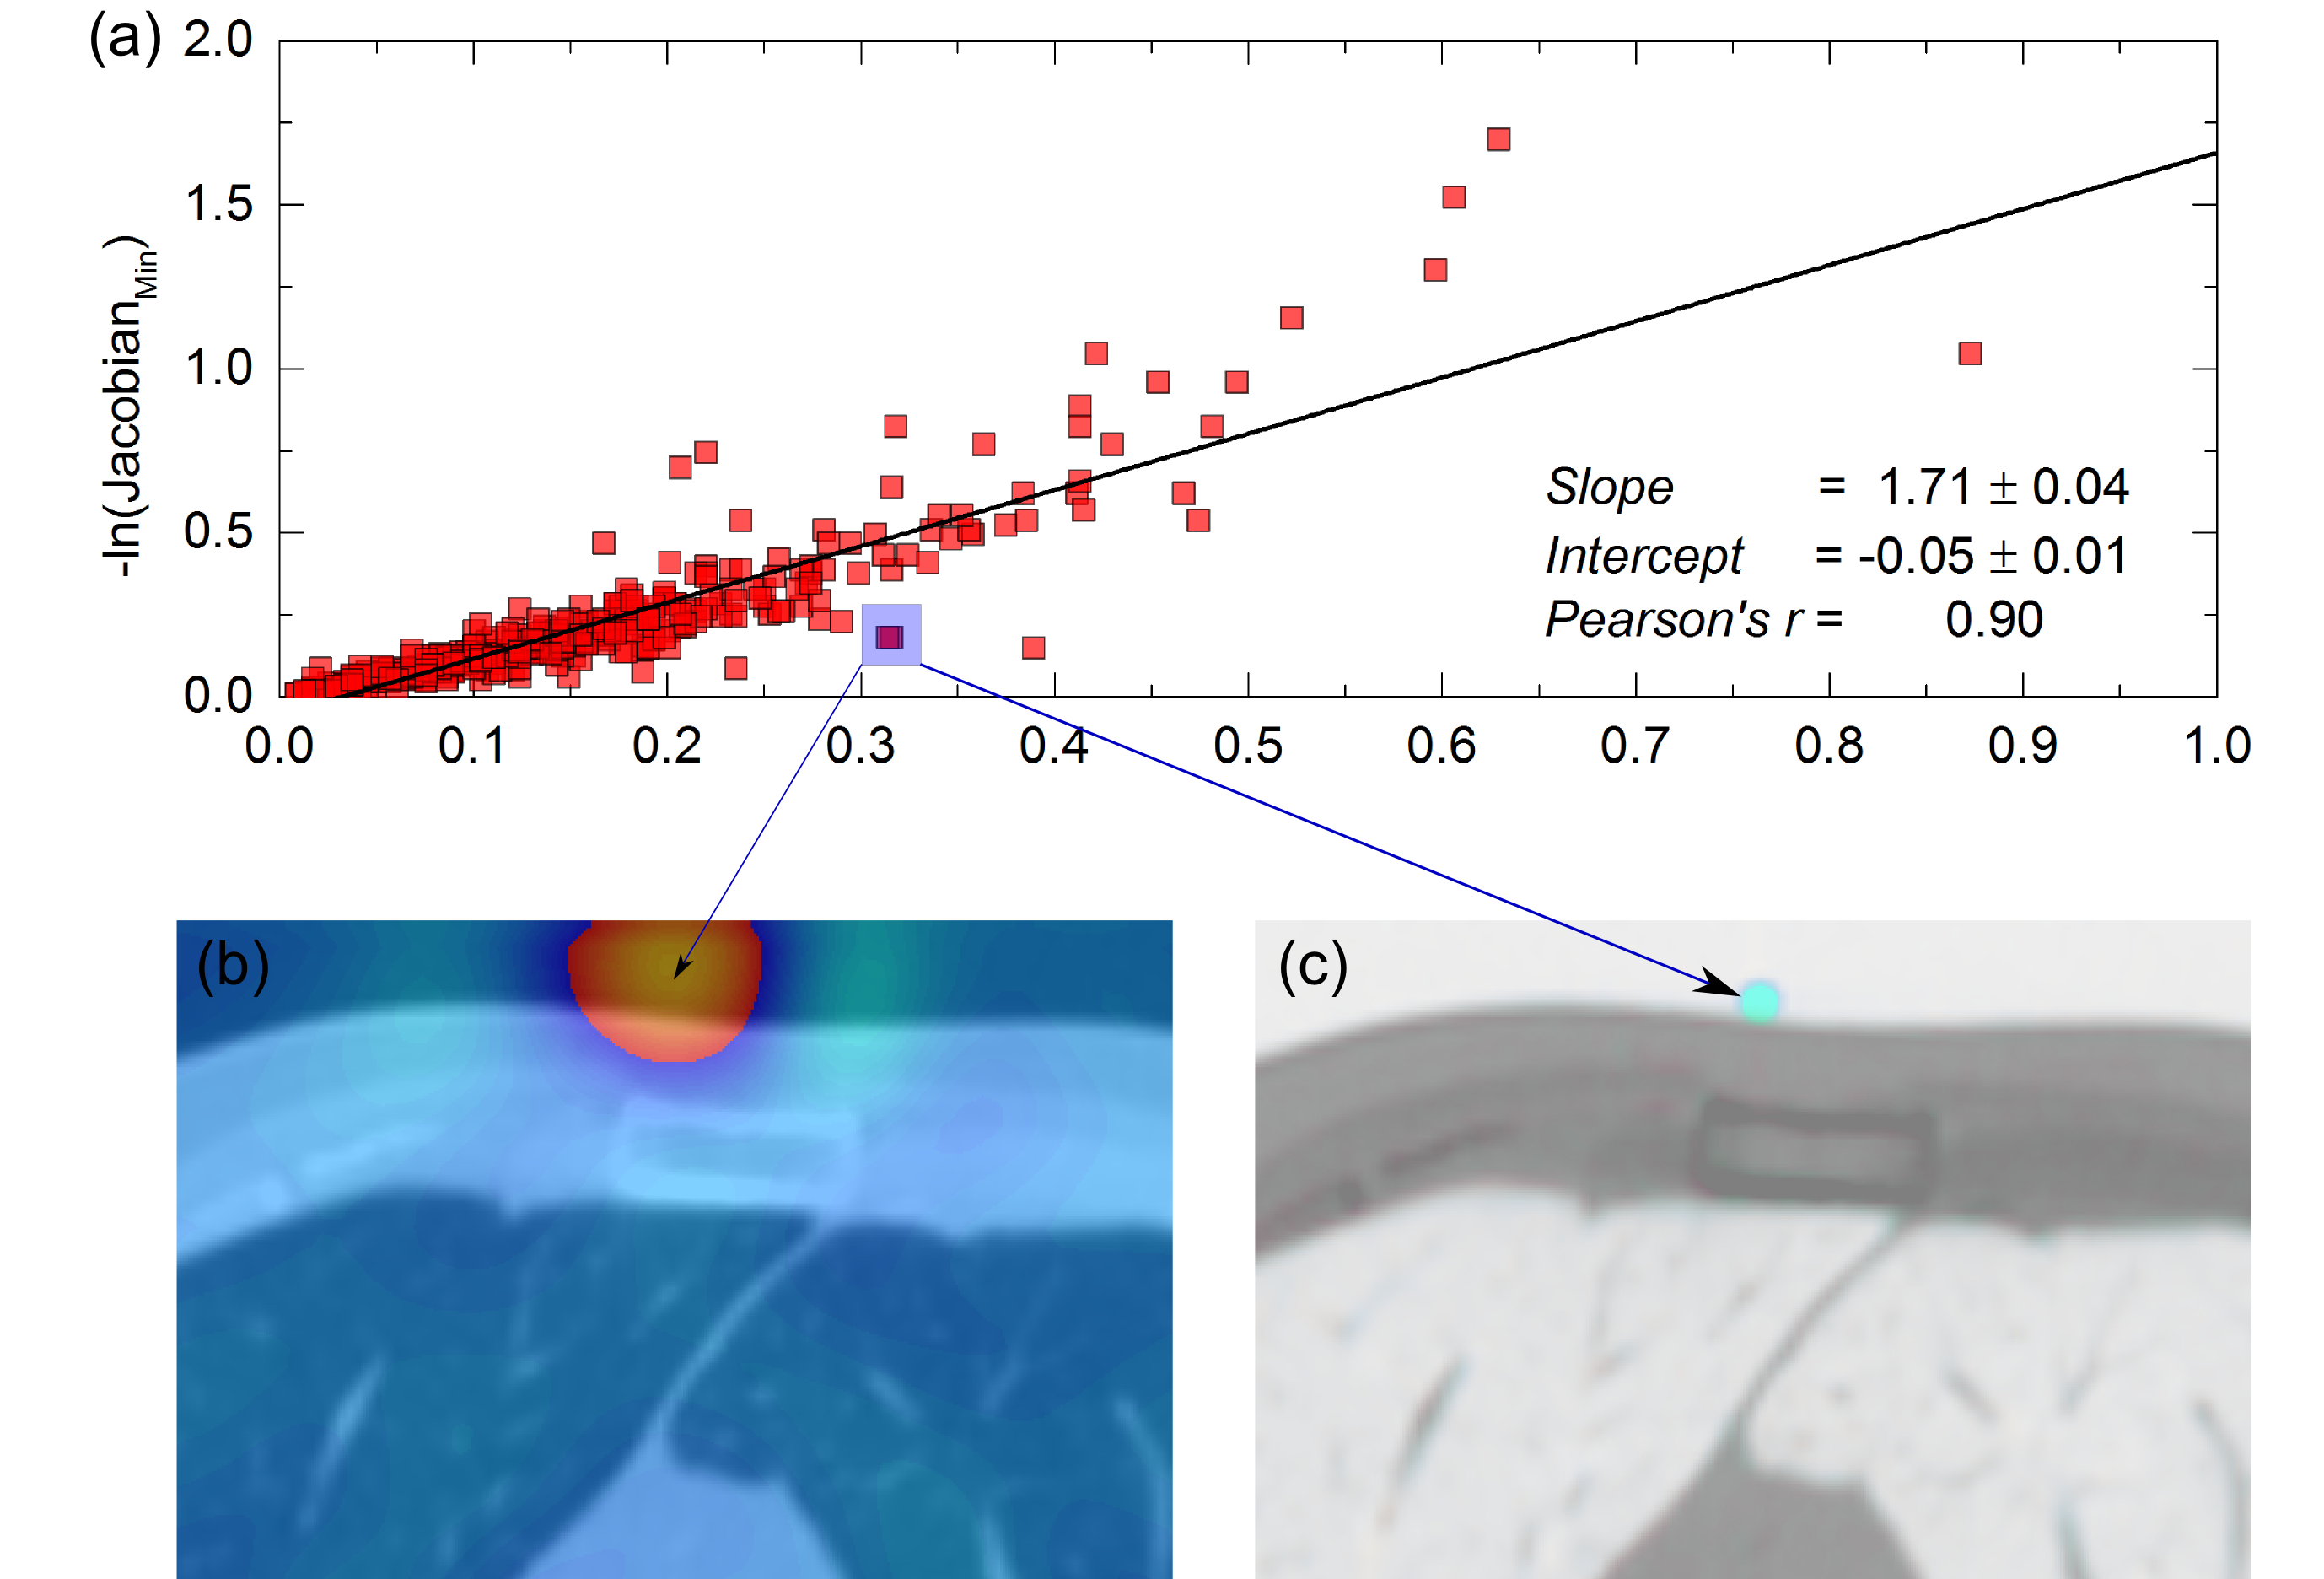
\includegraphics[width=0.8\textwidth]{./Vmm/Images/jacSum_lung.png}
% 		\caption{(a) Plot of negative natural logarithm of minimum inverse (true) Jacobian versus natural logarithm of maximum true (inverse) Jacobian. Linear fit is displayed with solid line and it's parameters are given in the corner. A deviation from linear fit (highlighted with blue square)
% 			was used as an example of scaled Jacobian (see text), shown in (b). (c) shows the CT the states highlighted in (a) in inverse color, where an artifact is clearly seen in one state and not the other.}
% 		\label{calcJac_lung}
% 	\end{center}
% \end{figure}

\newpage

\begin{figure}[H]
	\begin{center}		
		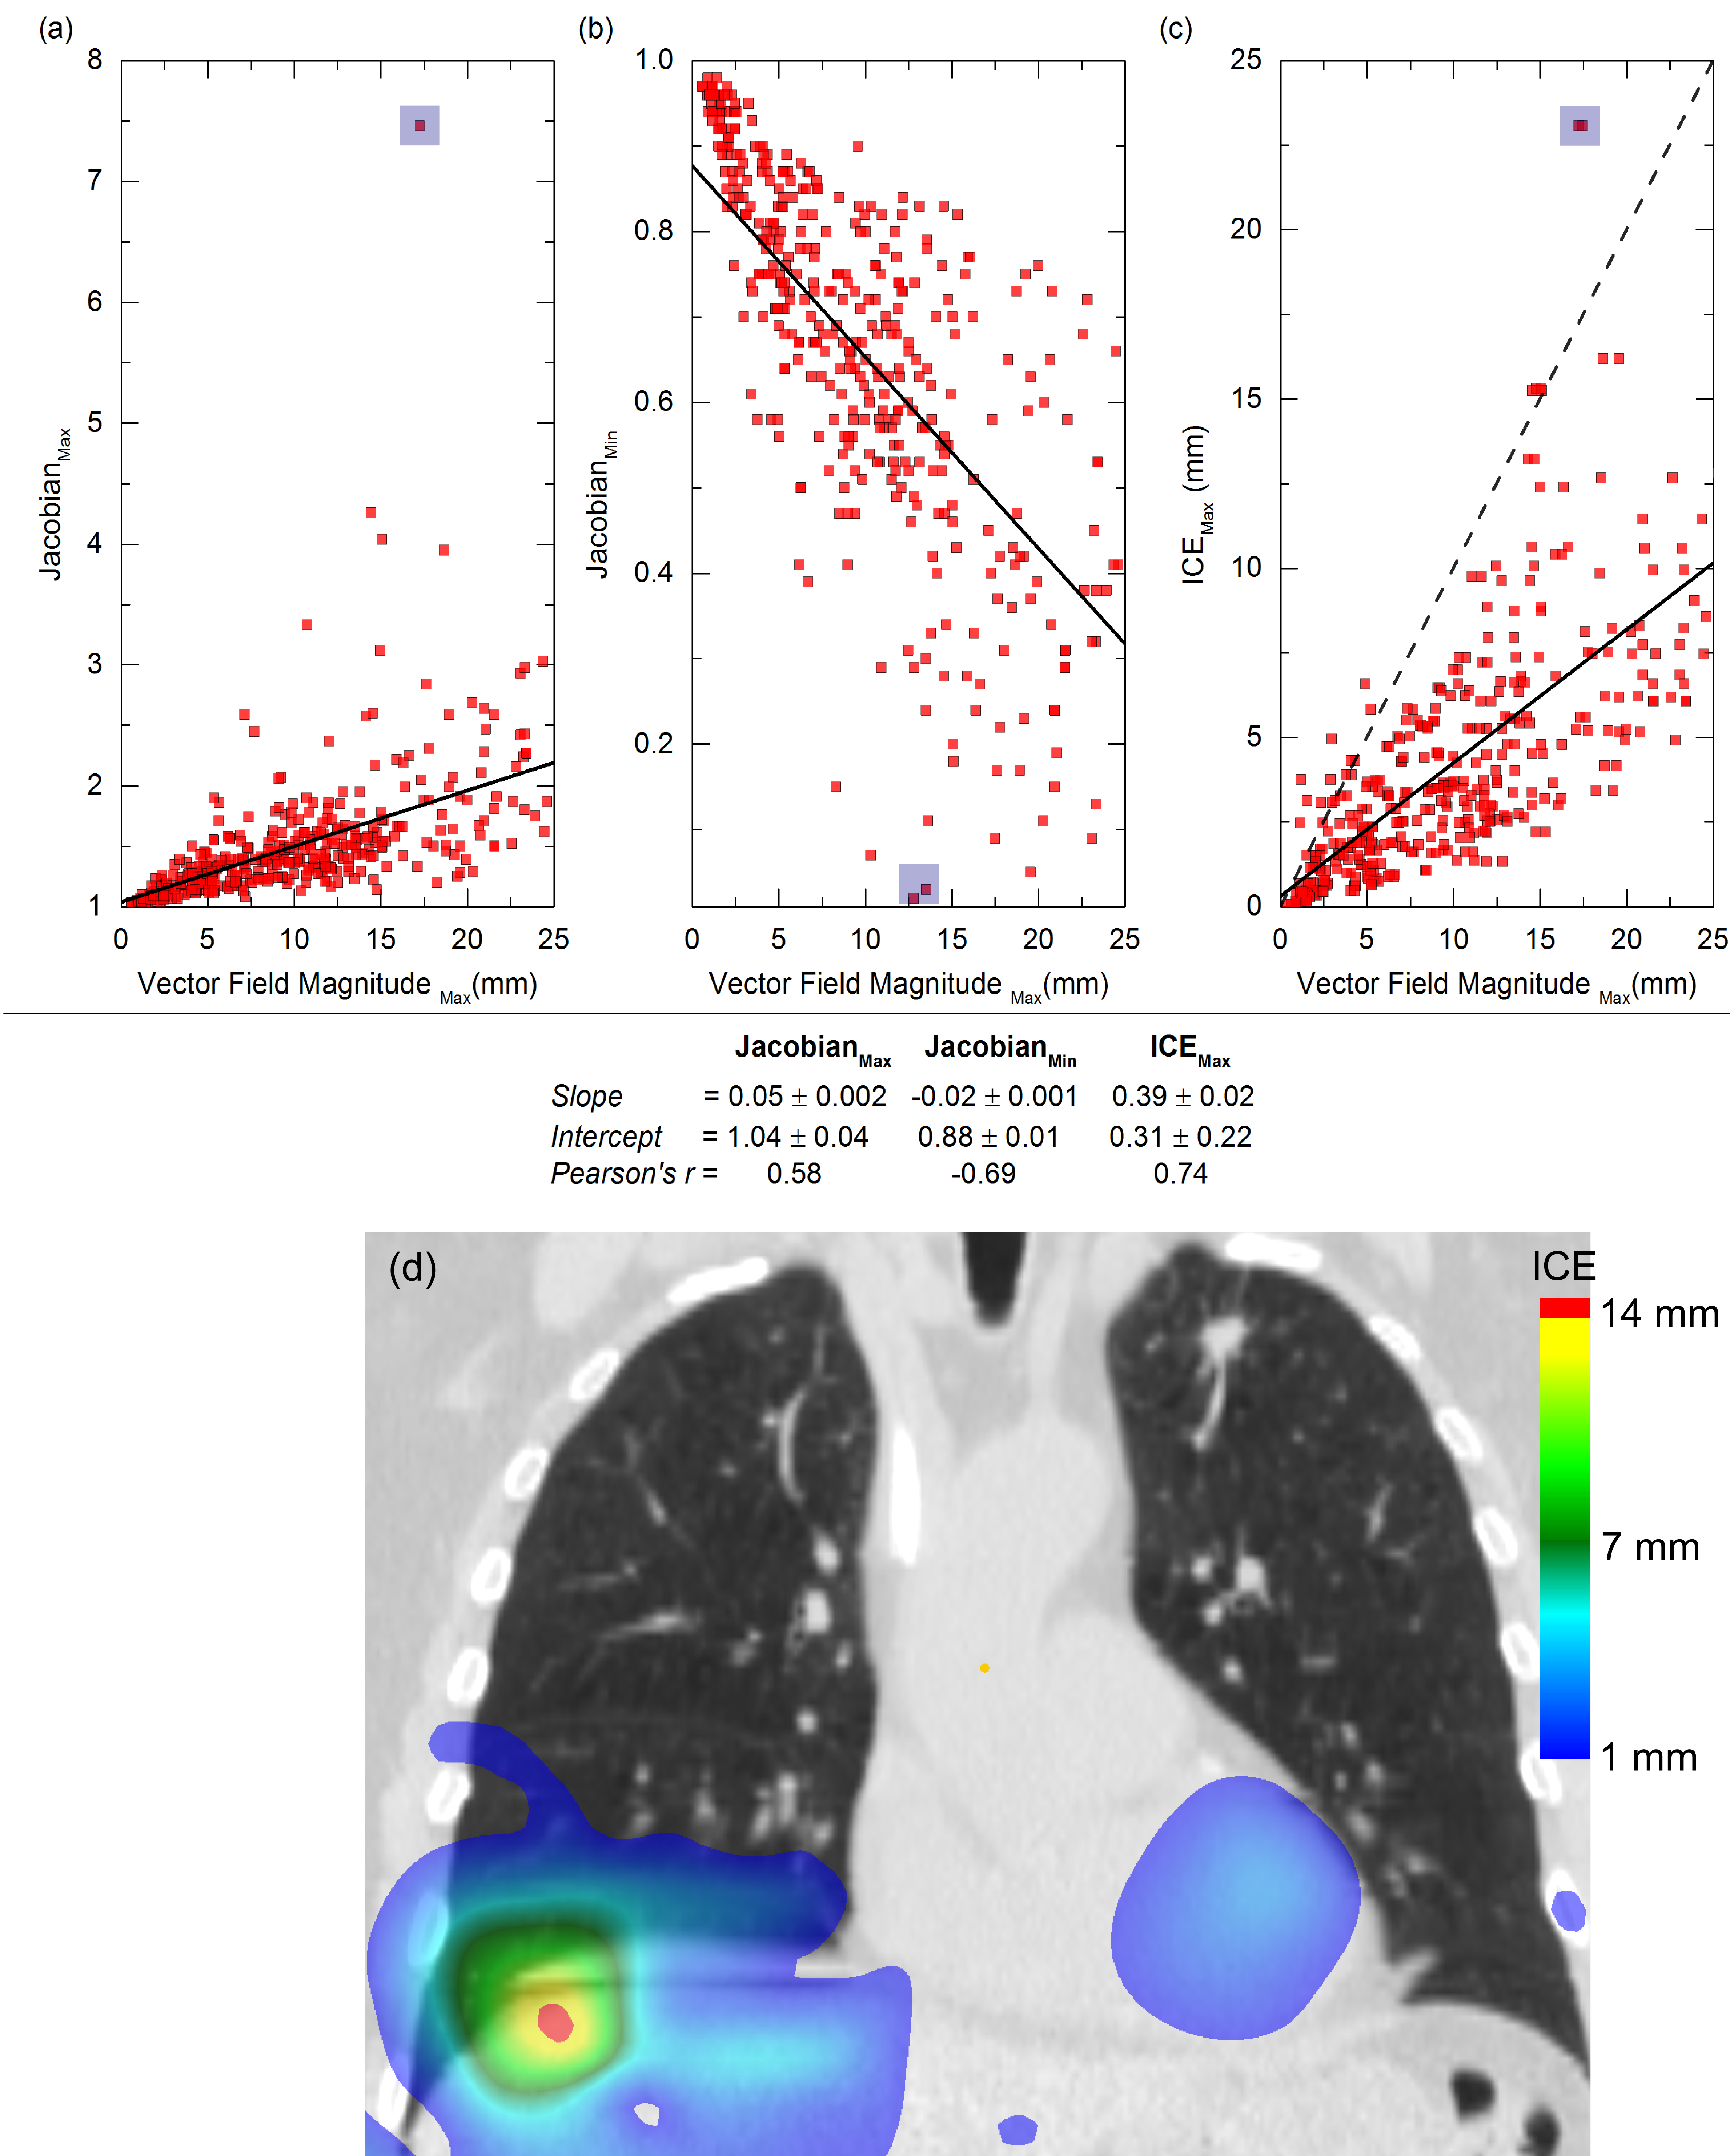
\includegraphics[width=0.9\textwidth]{./Vmm/Images/maxVf_lung.png}
		\caption{Values of maximum Jacobian (a), minimum Jacobian (b) and maximum ICE (c) plotted against maximum vector magnitudes. A linear fit is displayed with a solid line and parameters are written below the plots. Dashed line in (c) shows $y(x)= x$ plot.
			The points highlighted with blue squares come from the same DIR error that is shown in Fig.~\ref{contourPropagation}}
		\label{maxvf}
	\end{center}
\end{figure}

\newpage
\subsubsection{Discussion}
Nine states of 4D-CTs were registered to a 4D-CT reference state for 23 lung cancer patients, producing 414 true and inverse vector fields. All 414 DIR underwent a DIRQA consisting of vector field magnitudes, absolute difference, Jacobian and ICE.

Vector field magnitudes confirm previously published data that the biggest motion for lungs is in superior-inferior direction \cite{Seppenwoolde2002, Britton2007, Liu2007}. The mean vector field magnitude is small (in submilimiter range), 
because the ROI included the whole patient body, not just the lungs where most of the motion occurs. Vectors and inverse vectors are similar, which was expected.

There was a high correlation (Pearson's r = 0.87) between absolute difference before and after DIR. 
The slope of linear fit suggests that B-Spline DIR on average halves the absolute difference. There are several outliers from the
linear fit for default absolute difference bigger than 50 HU, however no DIR errors could be found upon visual inspection for this outliers.
All absolute differences after the DIR are smaller then before, which is a necessary condition in order for DIR to be considered successful. Apart from smaller absolute difference after DIR,
nothing could be deducted about the DIR quality from the absolute difference. The absolute difference is limited by the
image noise, which will always be present in a CT scan \cite{Polacin1992}. It would be interesting to study the 
correlation between image noise, absolute difference and consequential DIR quality.


Due to small mean vector field magnitudes, average values for true and inverse Jacobian were $1\pm0.05$, which indicates that most of the patient body does not change during the 4D-CT
scan. However, patient expansions and contractions can be seen on maximum and minimum Jacobian, with average values around 1.50 and 0.65 respectively. 
% If a part of a patient body contracts from reference to moving image, 
% then it expands in inverse direction and vice versa. The correlation was confirmed in Fig.~\ref{calcJac_lung}a, with a high Pearson's r (0.90). Furthermore outliers from linear fit spot inconsistencies
% in DIR as shown in Fig.~\ref{calcJac_lung}b and c, where a small artifact was found in one patient state solely from the deviation from linear fit in Fig.~\ref{calcJac_lung}. A scaled Jacobian could be used as a DIRQA check.

Mean and STD ICE are in submilimeter range, due to the correlation between vector field and ICE (see Eq.~\ref{eq:ice}). The maximum ICE (2.3 cm) was observed in a patient with 
an artifact present in state 2 of the 4D-CT, as shown in Fig.~\ref{maxvf}.
but still smaller as average maximum vector values. 

Large vector field magnitudes will produce more errors in DIR as shown in Fig~\ref{maxvf}. Linear fits were used to estimate increase (decrease) of Jacobian and ICE. 
As a rough DIRQA check, ICE should always be smaller than maximum vector field magnitudes. To confirm this, all cases above dashed line in Fig~\ref{maxvf}c 
were investigated and were found to have areas of poor DIR. An extreme case (highlighted in Fig.~\ref{maxvf}a-c)
had a large image artifact present in states 2 and 3 (state 3 with ICE is shown in Fig.~\ref{maxvf}d) leading to large inconsistencies in DIR. 
The effect of DIR inconsistency on contour propagation can be seen in Fig.~\ref{contourPropagation},
where lungs and liver contour were propagated using DIR. The propagated contours clearly differ from the image features.

The 4D-CT DIRs investigated here were used in particle therapy treatment planning. All areas that were found to have a poor DIR, were so far away from the target, that contour propagation or 4D dose calculation was not affected.
Hence a repetition of DIR was not necessary.
The patient in Fig.~\ref{contourPropagation} had a tumor in the upper left lung lobe and DIR inconsistencies were found in lower right lung lobe. 
Therefore all DIRs were considered successful. It should be stressed, however, that in this study only 4D-CTs that had a good contrast and no image artifacts in tumor vicinity were used.

\begin{figure}[H]
	\begin{center}		
		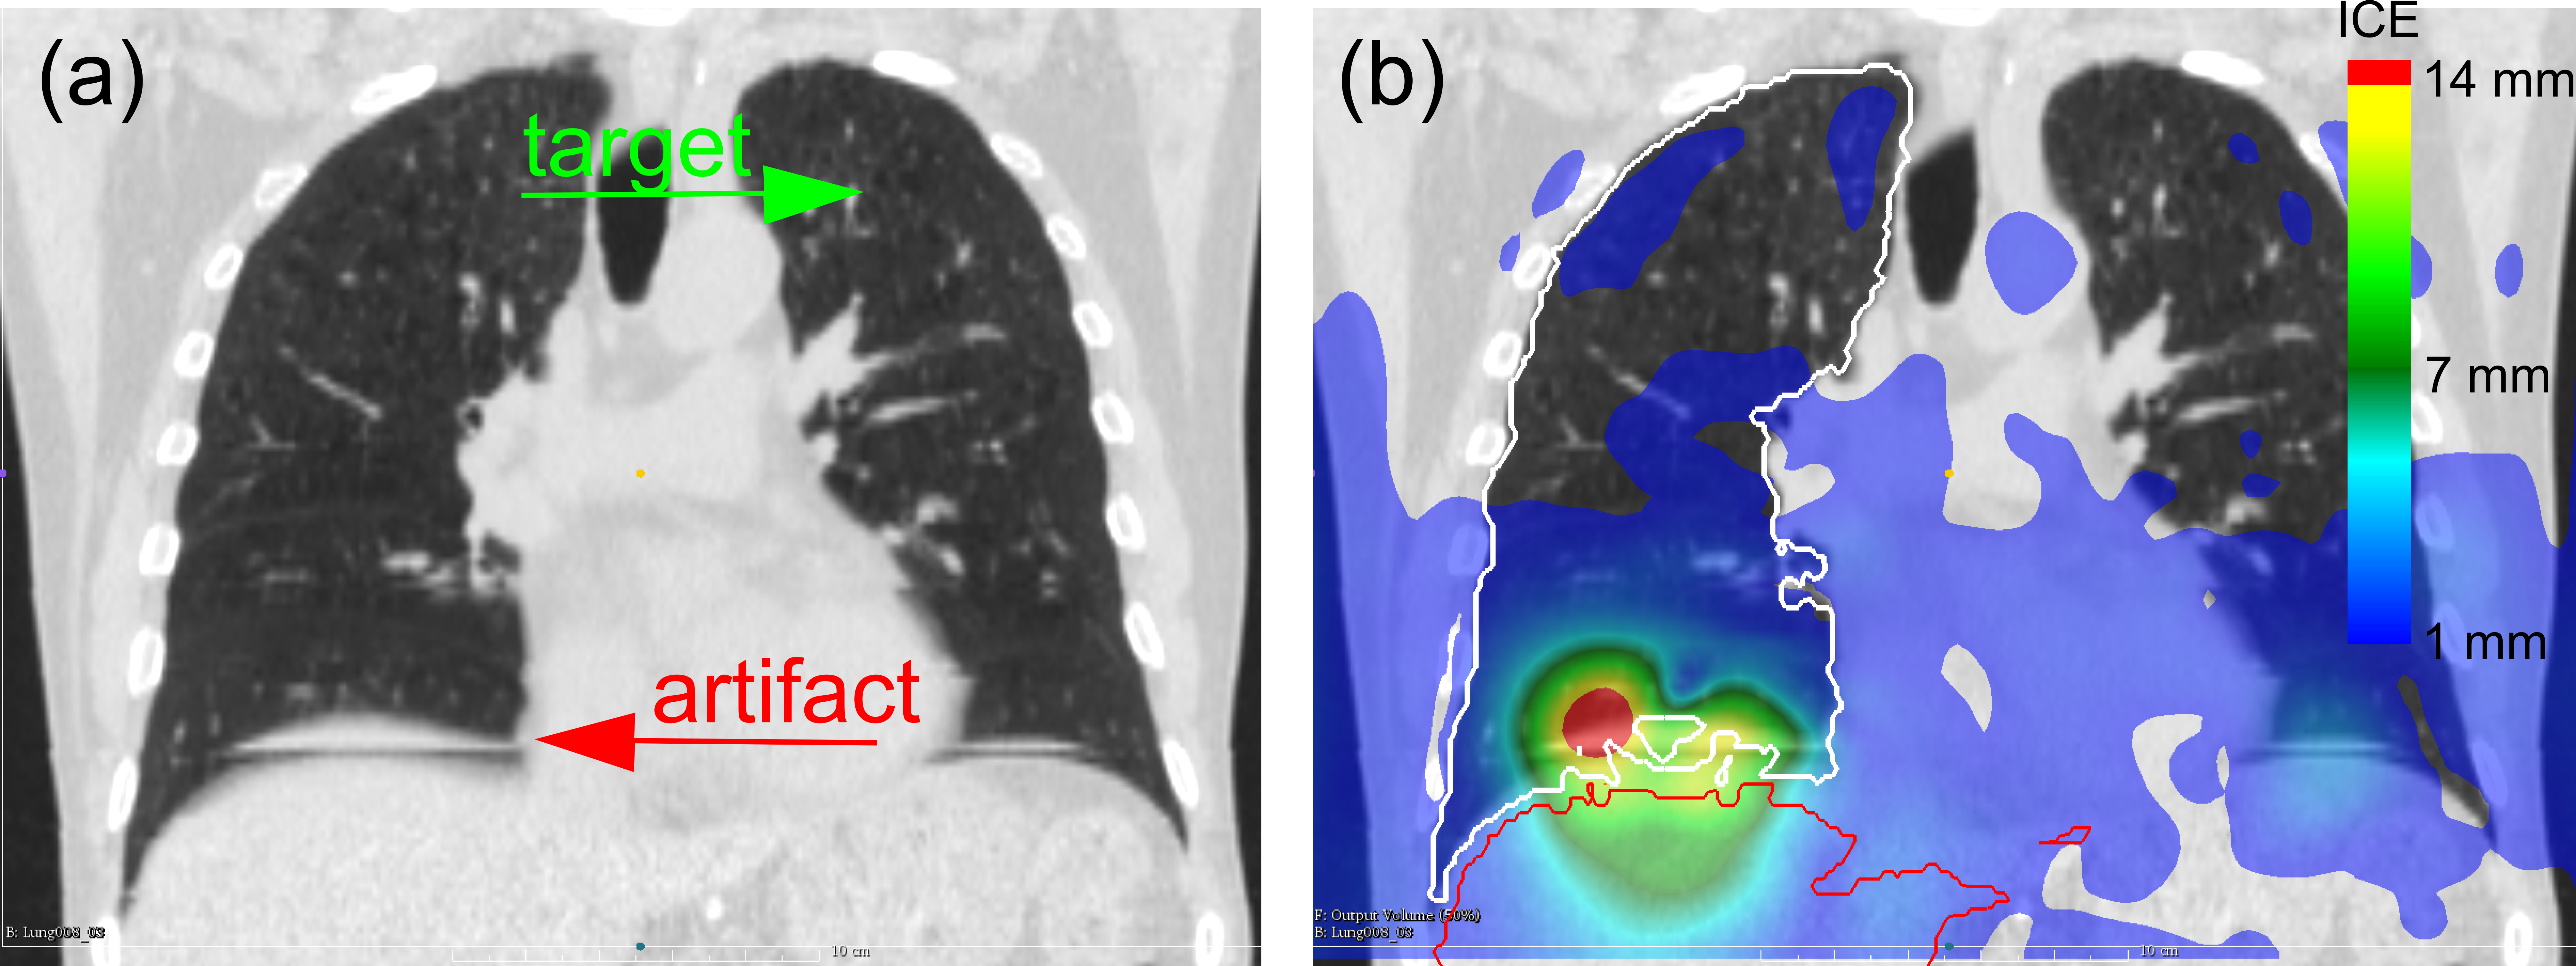
\includegraphics[width=0.9\textwidth]{./Vmm/Images/ContourPropagation/contourPropagation.png}
		\caption{Example of a contour propagation with an inconsistent DIR.(a) shows the location of 4D-CT artifact (red) and the location of the target (green). 
		The distance between them is big enough, that artifact does not affect treatment planning. 
		The large ICE is shown in (b) along with a propagated lung and liver contour. The errors in DIR result in a non-continuous diaphragm. Lungs are outlined in white and liver in red.}
		\label{contourPropagation}
	\end{center}
\end{figure}


\newpage
\subsection{Registration of pig heart 4D-CT data}

Atrial fibrillation is the most common type of cardiac arrhythmia, causing a quivering motion of the atrial small heart chamber. 
In itself it is not a life threatening, however it worsens the patients quality of life and increases the risk of a stroke \cite{Benjamin1998}. 
A common method for treating atrial fibrillation is catheter ablation \cite{January2014}. The success rate of catheter ablation is still limited and 
can lead to major complications or even death of a patient \cite{Cappato2005,Cappato2010}.

As an alternative treatment, a carbon-ion therapy was proposed \cite{Bert2012} and later feasibility on a beating heart was shown experimentally \cite{Lehmann2015b}. In 2014 a pilot experiment was performed at GSI using large animal model (pigs) and
scanned carbon-ion to verify the treatment in vivo \cite{Lehmann2015}.

To estimate and compensate motion of the heart during irradiation DIR of 4D-CT data was required. Furthermore, because of the actual irradiation of live pigs a DIRQA had to be made, to ensure the validity of DIR. Description of the procedure will be given here,
alongside with the results.


\subsubsection{Materials and Methods}


\subsubsection{Pig irradiation experiment}

DIR and DIRQA procedures will be given here, while a detailed description of the whole pig irradiation experiment can be found elsewhere \cite{Lehmann2015}. Cardiac gated contrast-enhanced CT scans (cardiac 4D-CT) were made on 15 pigs with a multidetector 64 row Siemens Somatom Definition Flash scanner 
(Siemens Healthcare, Forchheim, Germany) with 1 mm voxel and 1 mm slice spacing. There was no breathing motion present, since a breath-hold technique was used. Cardiac motion was based on electrocardiography (ECG)
and was divided into 10 sequential states (0-9). 
8 pigs had a pacemaker implemented, because the irradiation was planned to damage the atrioventricular (AV) node and a pacemaker should compensate for that. Pigs are therefore divided into two groups, with pacemaker (PM), $n=8$, and without one (noPM), $n=7$.

After CT acquisition, DIR on cardiac 4D-CT was made using B-Spline Plastimatch module in Slicer (see Section~\ref{RegistrationImplement}). 
Details on parameters used for DIR can be found in Table~\ref{tab:stages2}. State 0 was chosen as a reference state. State 3 corresponds to a maximum heart contraction with likely
the biggest motion. All other states were registered to the reference state with inverse registration as well. 
A checklist was made to follow DIR and DIRQA for quality assurance. An example of a filled-out checklist is shown in Fig.~\ref{checkList}a.

Based on lung patient DIR and because of the time constraints in the study workflow, DIRQA was made only on DIR from state 5. 
DIRQA consisted of default and true absolute differences, true Jacobian and ICE. DIRQA results were stored in a text file (example shown in Fig.~\ref{checkList}b) and users checked if the values did not exceed expected ones: Mean absolute difference
should be smaller than 1; mean Jacobian  should be 1; mean ICE  should be smaller than 2 mm. A box-shaped ROI was created in Slicer to encompass the pig body and then used in all DIRQA checks.

After a successful DIR and DIRQA, vector fields were used in a treatment planning and the resulting plans were used in the pig irradiation experiment.

Around 20 minutes were needed for each pig DIR and additional 20 minutes for pig DIRQA. Calculations were done on a Linux computer with 8 CPU cores and 32 GB RAM.

\begin{table}[H]
  \centering
%   \footnotesize
  \caption{Parameters used for Plastimatch registration.  A mean squared error metric was used. Details for each parameter can be found here \cite{Plastimatch}.}
  \begin{tabular}{c|c|c}
      Parameter & Stage 1 & Stage 2 \\
      \hline
      Resolution & 4,4,2 & 2,2,1 \\
      Grid size & 50 & 15 \\
      Regularization lambda & 0.005 & 0.005 \\
      Iterations & 200 & 100 \\
    \hline\hline
  \end{tabular}
  \label{tab:stages2}
\end{table}

\subsubsection{Post-experiment analysis}

After the conclusion of the animal study, a more detailed DIRQA was made, with all motion states included in DIRQA. In addition to original checks explained in previous section, vector field magnitudes were analyzed, inverse absolute difference
and Jacobian were calculated. Paired t-tests were used to test statistical significance for vector field magnitudes between true and inverse vector fields and PM and noPM groups. For linear fit quality estimation, 
a Pearson's r coefficient was used.

\newpage
\begin{figure}[H]
	\begin{center}		
		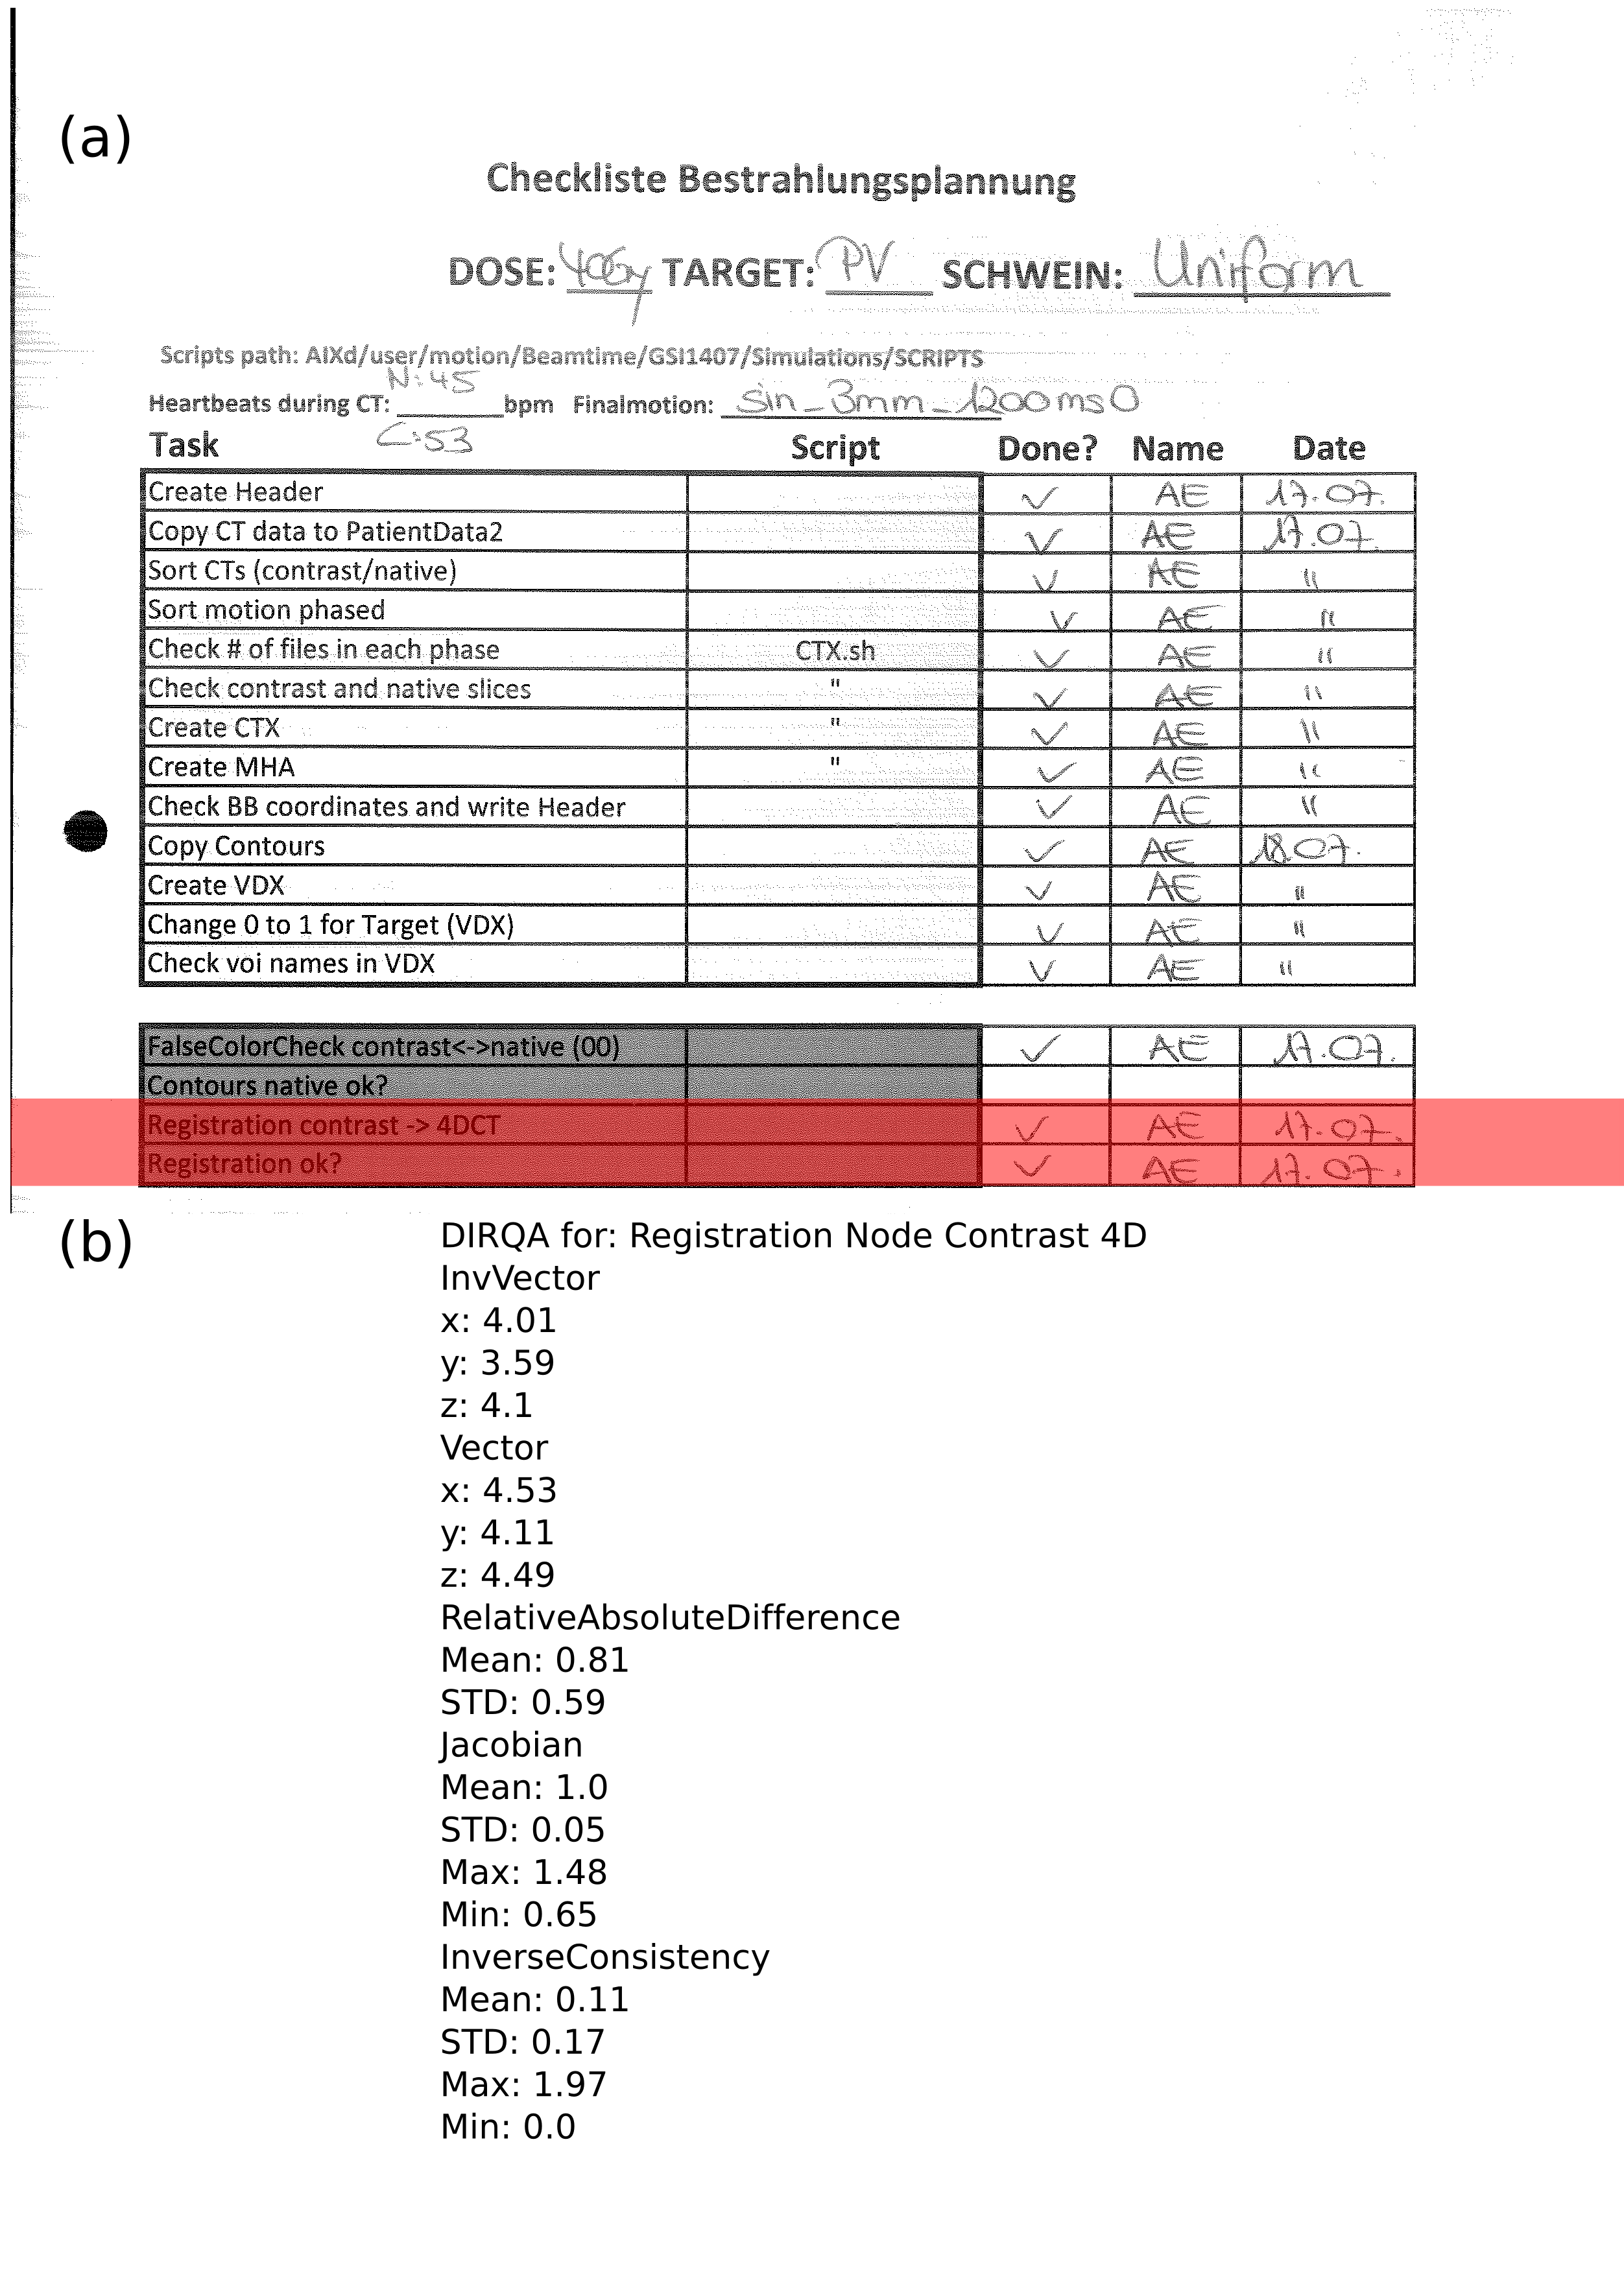
\includegraphics[width=0.8\textwidth]{./Vmm/Images/checkList.png}
		\caption{(a) Part of the checklist for quality assurance during pig irradiation. DIR and DIRQA part is highlighted in red and consisted of two steps. First DIR was made on cardiac 4D-CT and afterwards DIRQA was made on
		DIR from state 50\%. End result was presented as text shown in (b). Relative absolute difference stands for ratio between true and default absolute difference.}
		\label{checkList}
	\end{center}
\end{figure}
\newpage
\begin{figure}[H]
	\begin{center}		
		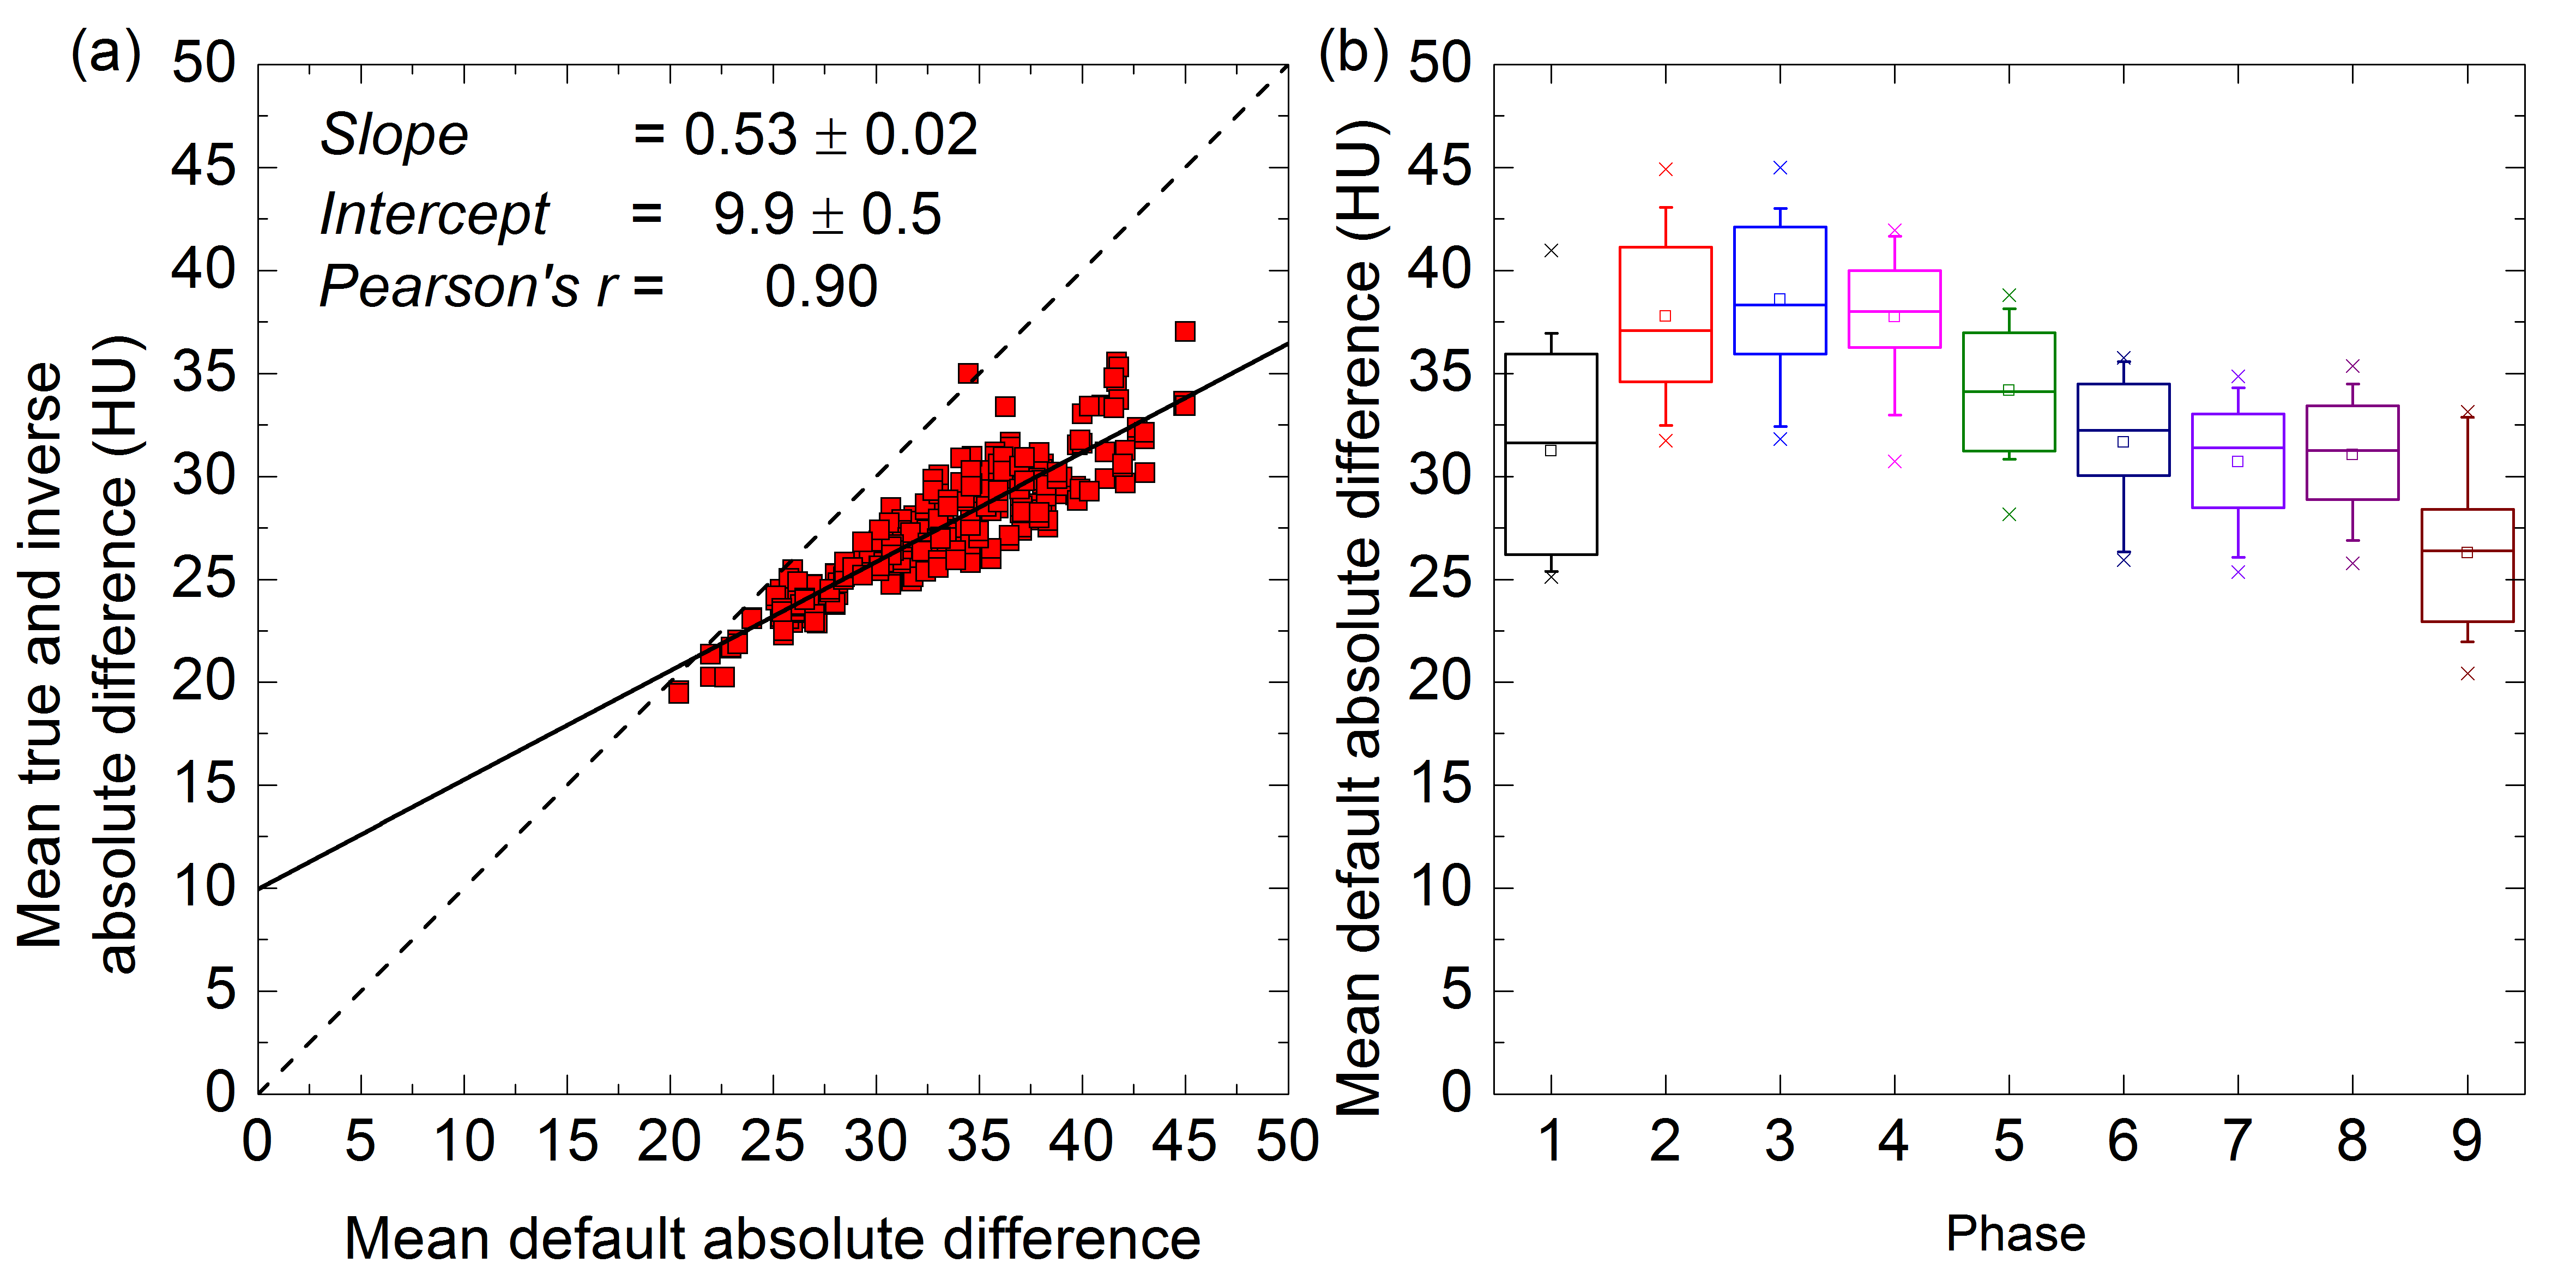
\includegraphics[width=0.9\textwidth]{./Vmm/Images/AbsDiff_pigs.png}
		\caption{(a) Mean true and inverse absolute difference plotted against mean default absolute difference. Solid line shows linear fit, with parameters
		written in corner. Dashed line shows $y(x)=x$. (b) Box plots of mean default absolute difference distribution across nine 4D-CT states. Boxes represent 25-75\%, whiskers 10-90\%
		of data, median is shown with a solid line, mean with squares and outliers with crosses.}
		\label{absDiff_pigs}
	\end{center}
\end{figure}

\subsubsection{Results}

An example of a pig cardiac 4D-CT DIR is shown in Fig.~\ref{exampleReg_pigs}. One DIRQA during the animal study showed higher mean true absolute difference than mean default absolute difference. The registration
was therefore repeated with three stages instead of 2. The third stage had 100 iterations with resolution size ``1, 1, 1`` and grid size ''10``. All other DIRQA checks were positive.

A post-experiment statistical analysis on vector field magnitudes is shown in Table~\ref{tab:vectordata_pig}. No statistical difference was
observed between true and inverse vector fields. However, significant differences were observed between vector field magnitudes of PM and noPM groups. Contributions to vector field magnitudes from three axis were equal. 


\begin{table}[H]
  \centering
%   \footnotesize
  \caption{Data for vector magnitudes. Values are presented as mean (range).}
  \begin{tabular}{c|c|c|c|c}
	    & \multicolumn{2}{|c|}{PM} & \multicolumn{2}{|c}{noPM} \\
  
            & True vector field   & Inverse vector field   & True vector field  & Inverse vector field \\
       \hline
	Mean & 0.08 (0.03 - 0.16) & 0.08 (0.03 - 0.14) & 0.07 (0.0 - 0.18)  & 0.06 (0.0 - 0.17) \\ 
	STD  & 0.4 (0.09 - 0.78)  & 0.36 (0.08 - 0.68) & 0.3 (0.05 - 0.77)  & 0.28 (0.04 - 0.71) \\ 
	Max  & 8.24 (1.6 - 17.33) & 7.98 (0.7 - 17.76) & 5.9 (0.97 - 15.91) & 5.38 (1.08 - 12.42) \\ 
    \hline\hline
  \end{tabular}
  \label{tab:vectordata_pig}
\end{table}

\begin{figure}[H]
	\begin{center}		
		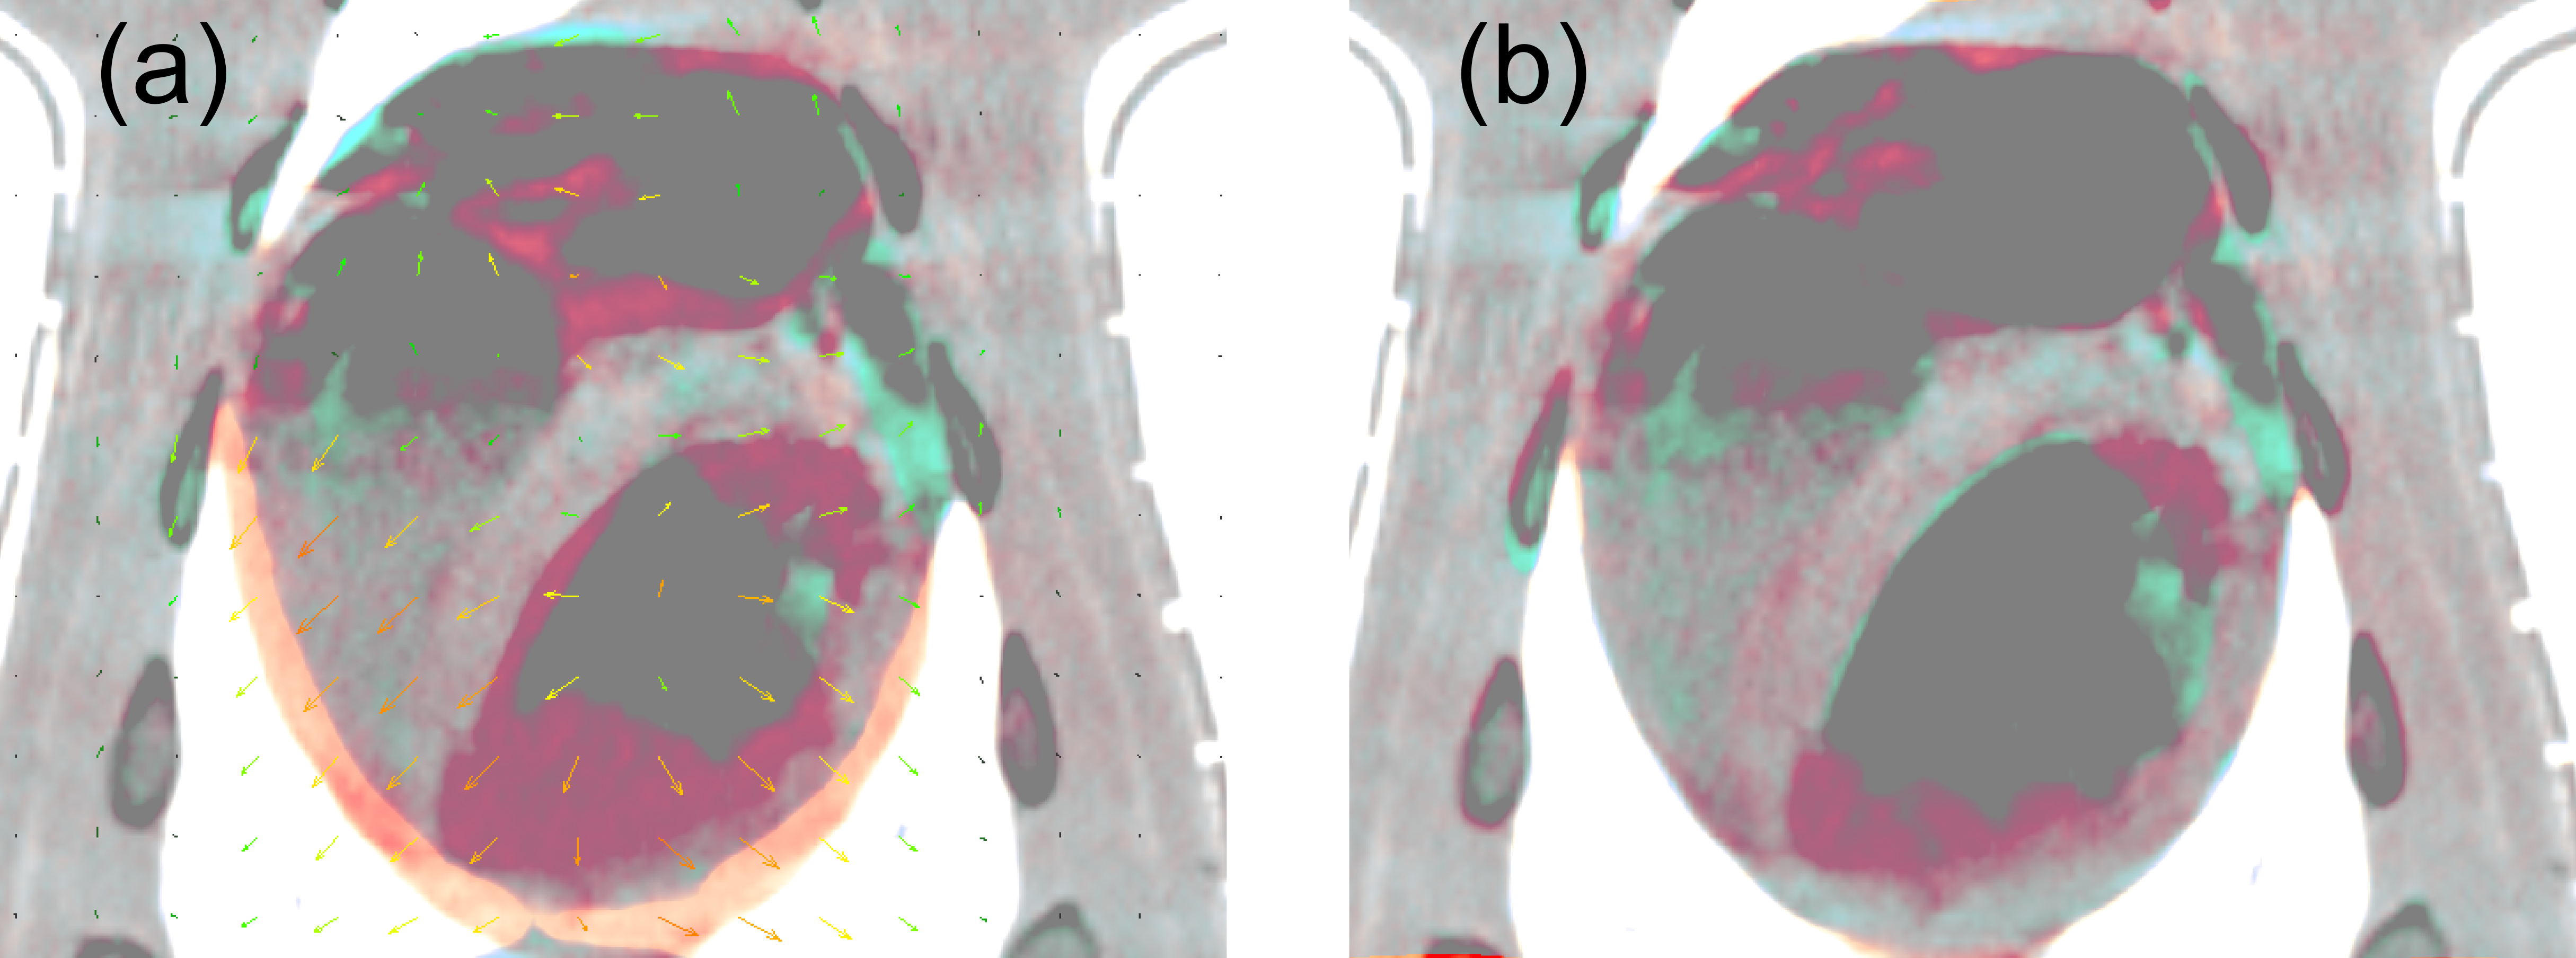
\includegraphics[width=0.9\textwidth]{./Vmm/Images/exampleReg_pigs.png}
		\caption{Inverse color overlay of two states before (a) and after (b) DIR. Vector field is displayed on image (a) as arrows.}
		\label{exampleReg_pigs}
	\end{center}
\end{figure}

The dependence of true and inverse absolute difference on default absolute difference with a linear fit is shown in Fig.~\ref{absDiff_pigs}a. 
Default absolute difference distribution across 9 states can be seen in Fig.~\ref{absDiff_pigs}b.

Distribution of Jacobian and ICE results are shown in Fig.~\ref{jacobian_data_pigs}. Maximum values of true and inverse Jacobian and maximum ICE were
tested against maximum vector magnitudes and fitted with linear function. Results are plotted in Fig.~\ref{maxvf_pigs}.

All linear fits in Fig.~\ref{absDiff_pigs} and ~\ref{maxvf_pigs} were statistically significant (p < 0.05).



\newpage

\begin{figure}[H]
	\begin{center}		
		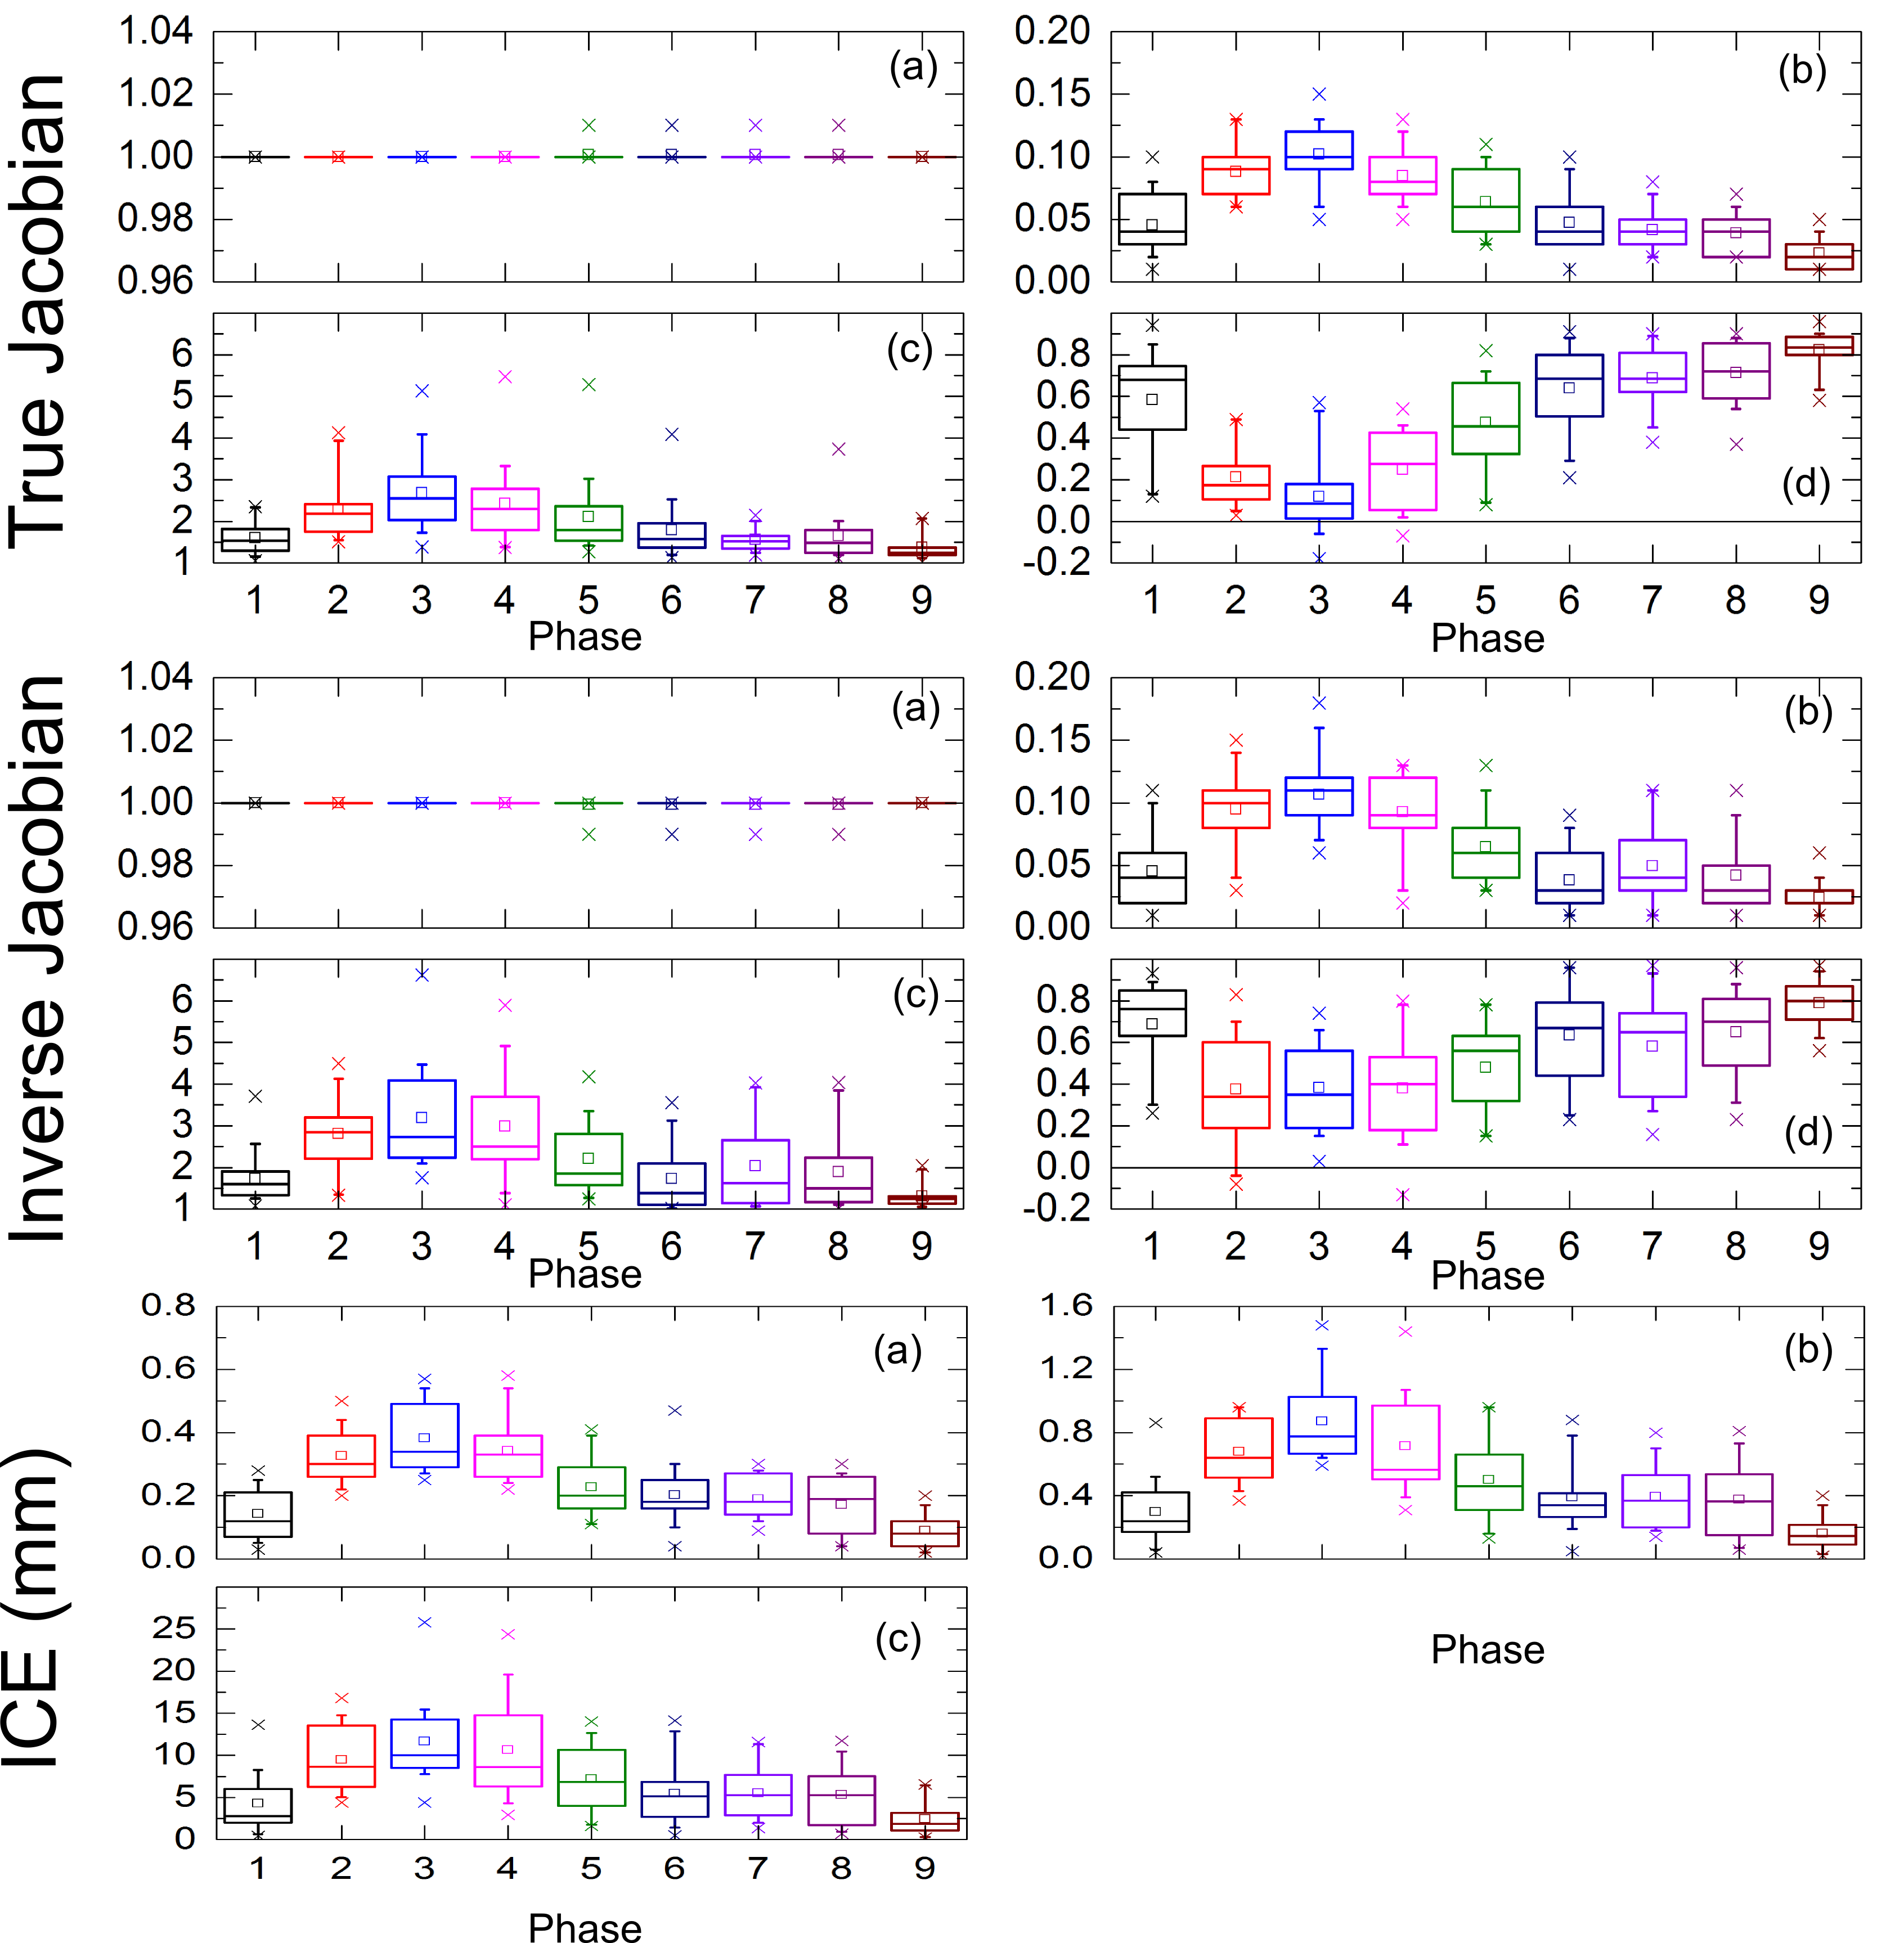
\includegraphics[width=0.75\textwidth]{./Vmm/Images/Jacobian_data_pigs.png}
		\caption{Statistical data for true (top) and inverse (middle) Jacobian and ICE (bottom) for 9 cardiac 4D-CT states (reference state 0 is excluded) for 15 pigs. Mean, STD, maximum and minimum are represented as (a), (b), (c) and (d), respectively.
		Minimum ICE is 0 throughout all states and pigs. Boxes represent 25-75\%, whiskers 10-90\% of data, median is shown with a solid line, mean with squares and outliers with crosses.}
		\label{jacobian_data_pigs}
	\end{center}
\end{figure}

\newpage

% \begin{figure}[H]
% 	\begin{center}		
% 		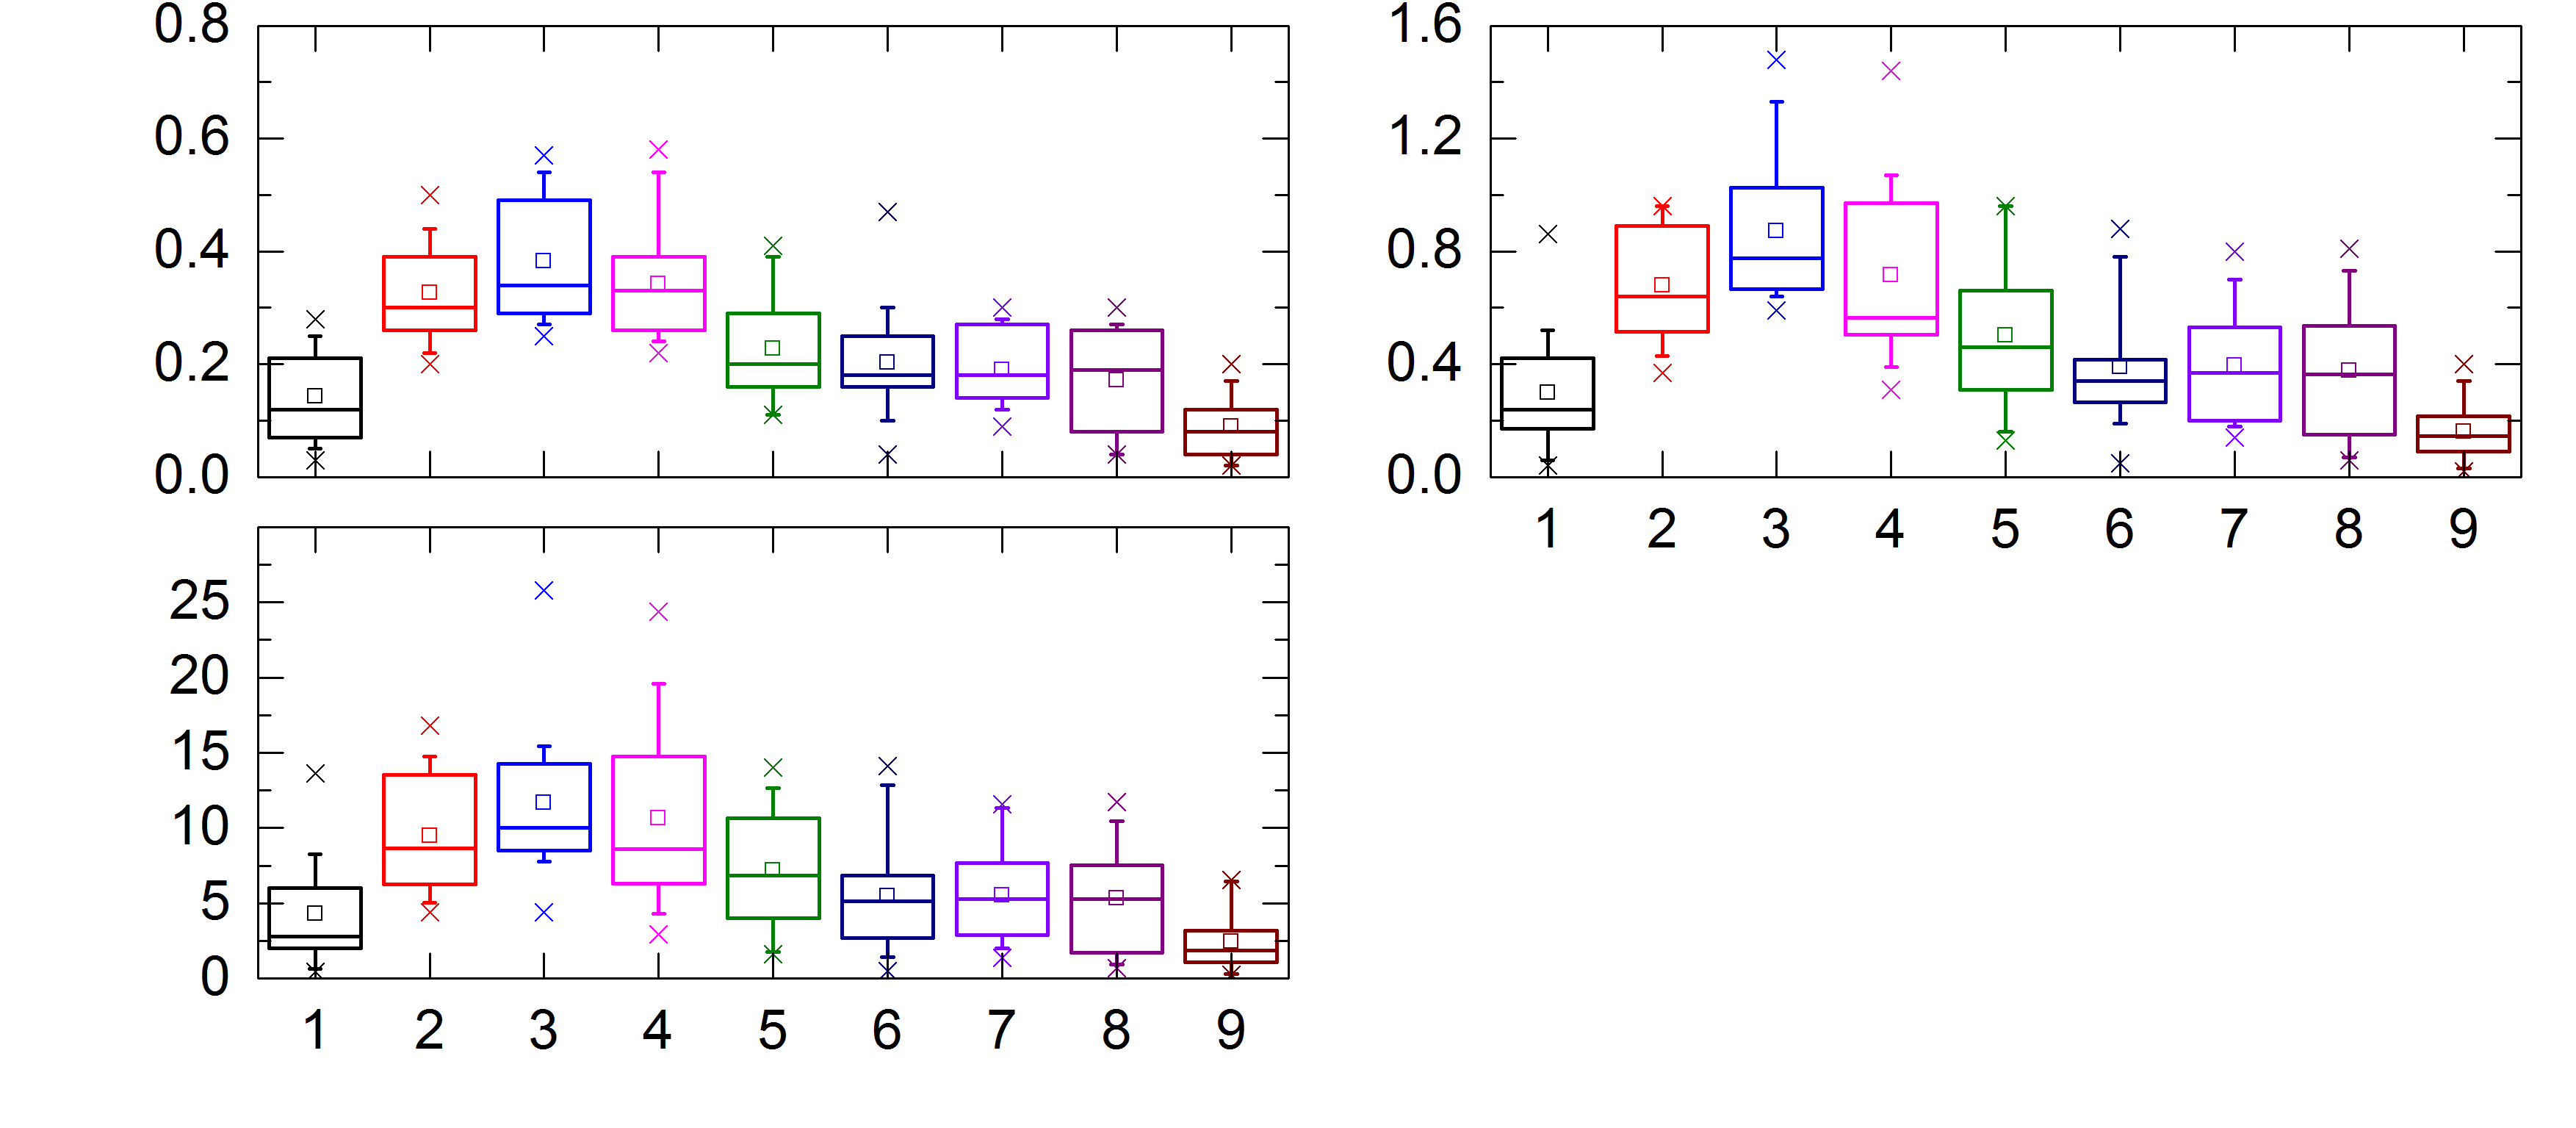
\includegraphics[width=0.9\textwidth]{./Vmm/Images/ICE_pigs.png}
% 		\caption{Statistical data for ICE for 9 4D-CT states (reference state 0 is excluded) for 15 pigs. Mean, STD, maximum are represented as (a), (b) and (c), respectively. 
% 		Boxes represent 25-75\%, whiskers 10-90\% of data, median is shown with a solid line, mean with squares and outliers with crosses.}
% 		\label{ice_pigs}
% 	\end{center}
% \end{figure}

% \begin{figure}[H]
% 	\begin{center}		
% 		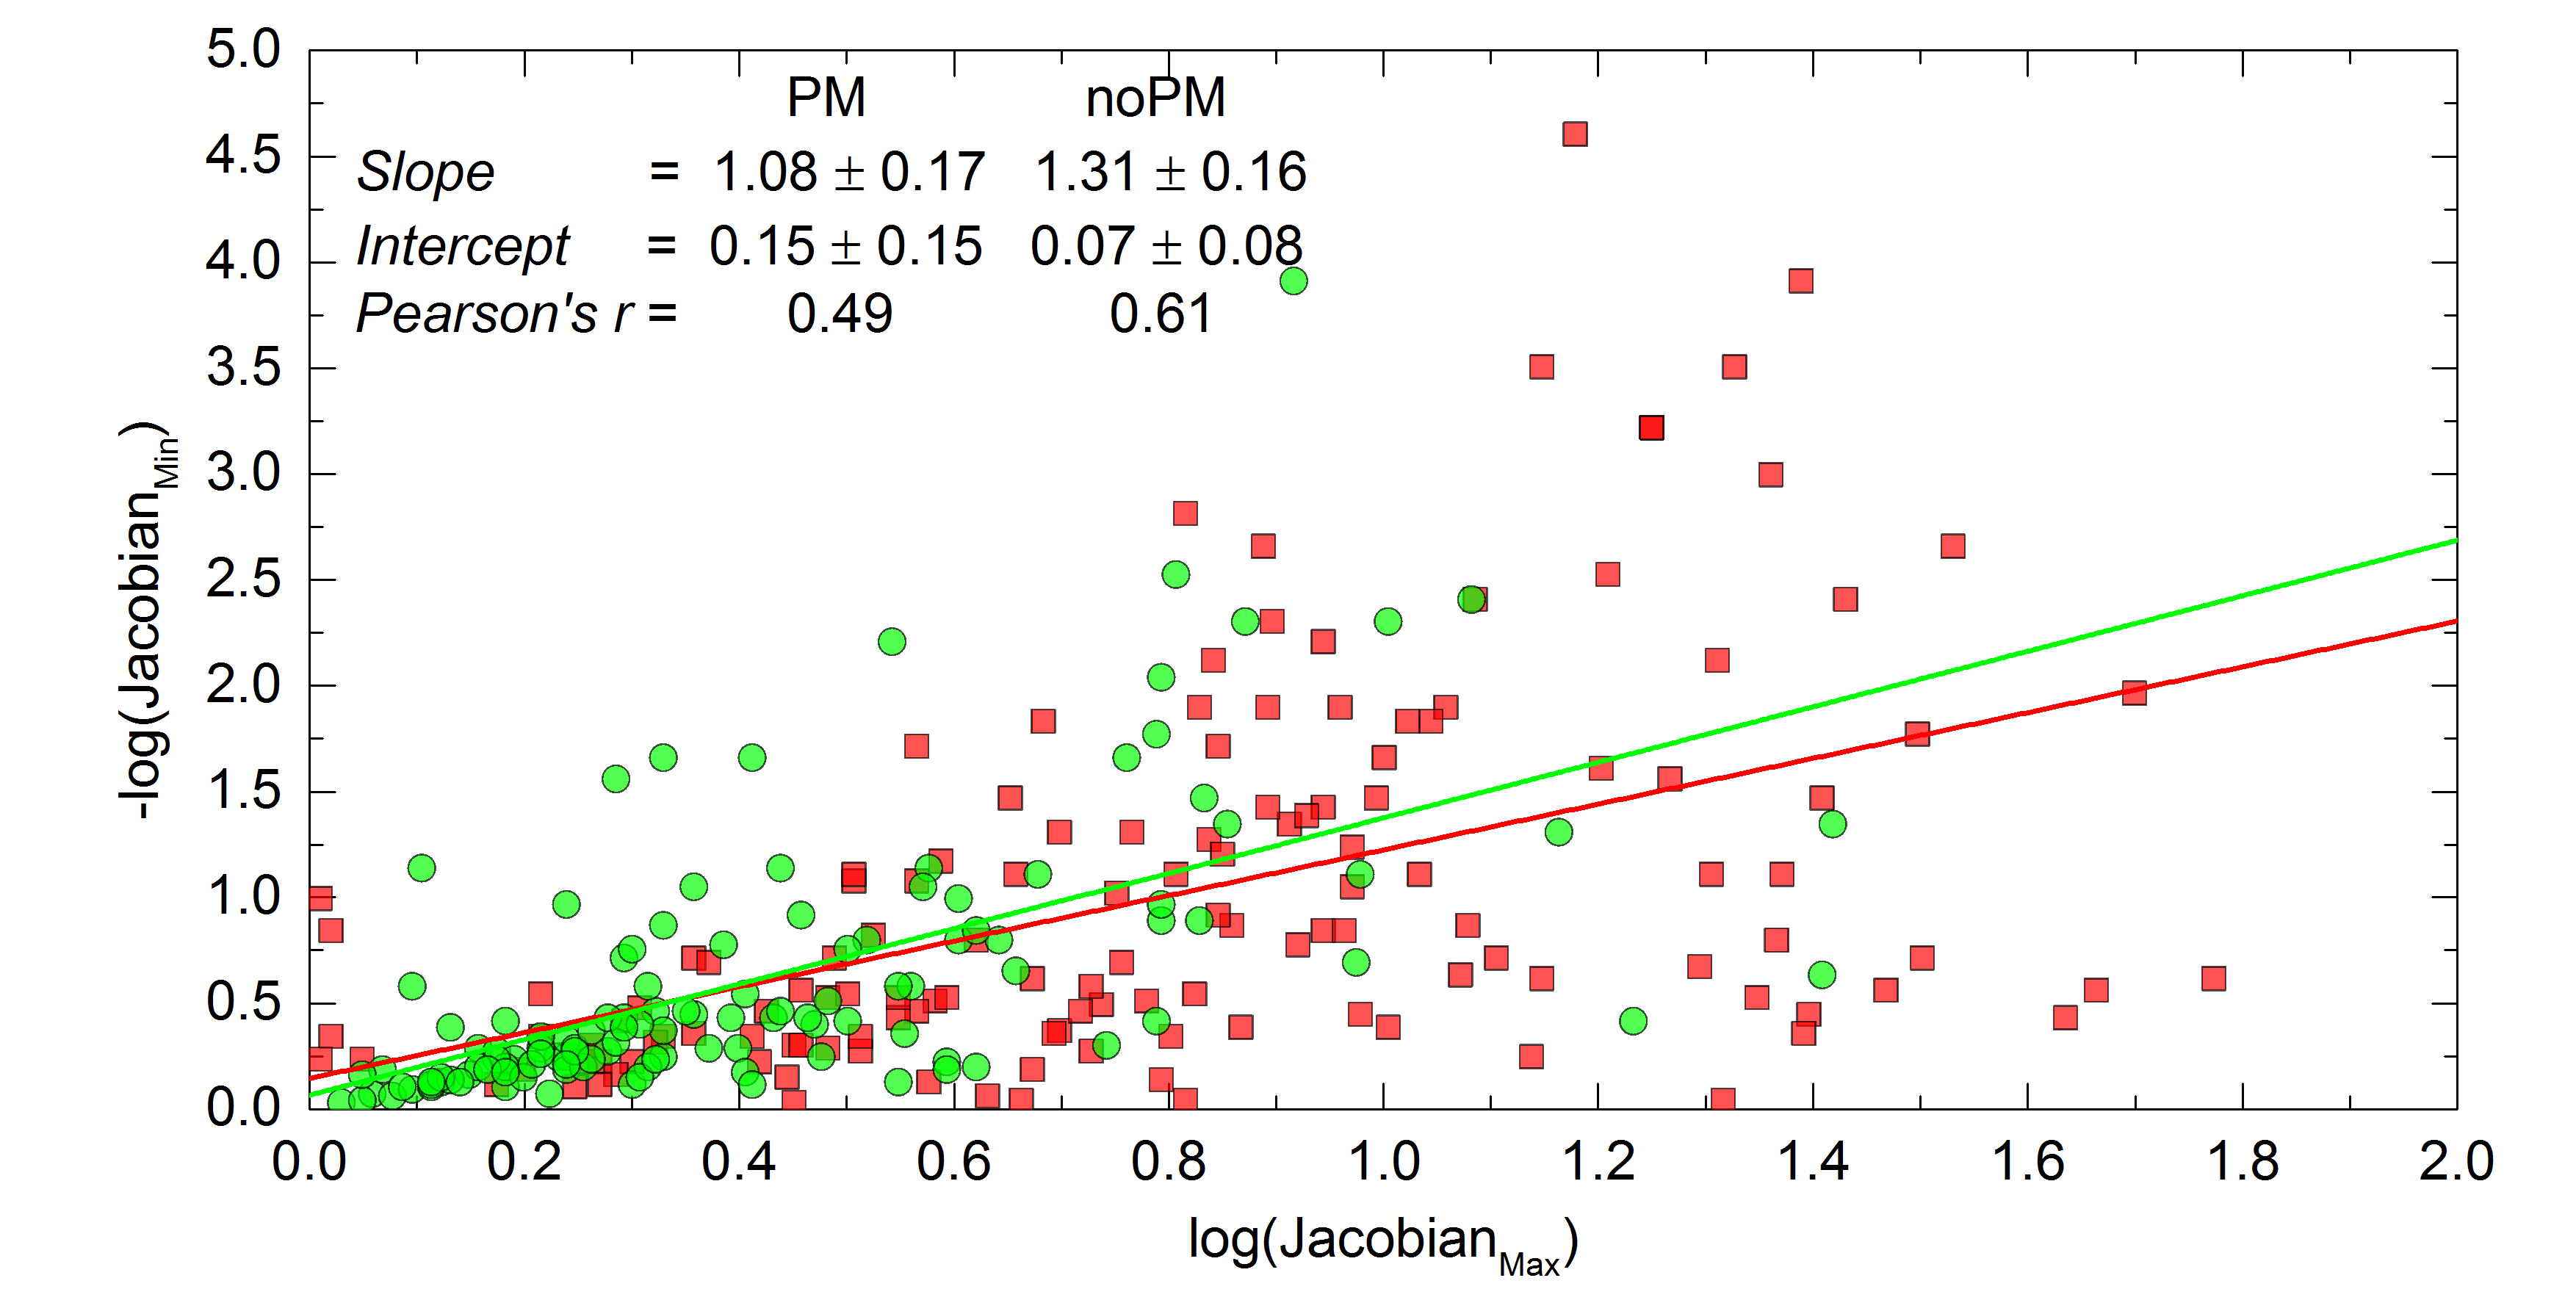
\includegraphics[width=0.9\textwidth]{./Vmm/Images/JacSum2.png}
% 		\caption{(a) Plot of negative natural logarithm of minimum Jacobian versus natural logarithm of maximum Jacobian. Linear fit is displayed with solid line and it's parameters are given in the corner. PM and noPM are shown with red squares and green circles, respectively.}
% 		\label{calcJac_pigs}
% 	\end{center}
% \end{figure}

\begin{figure}[H]
	\begin{center}		
		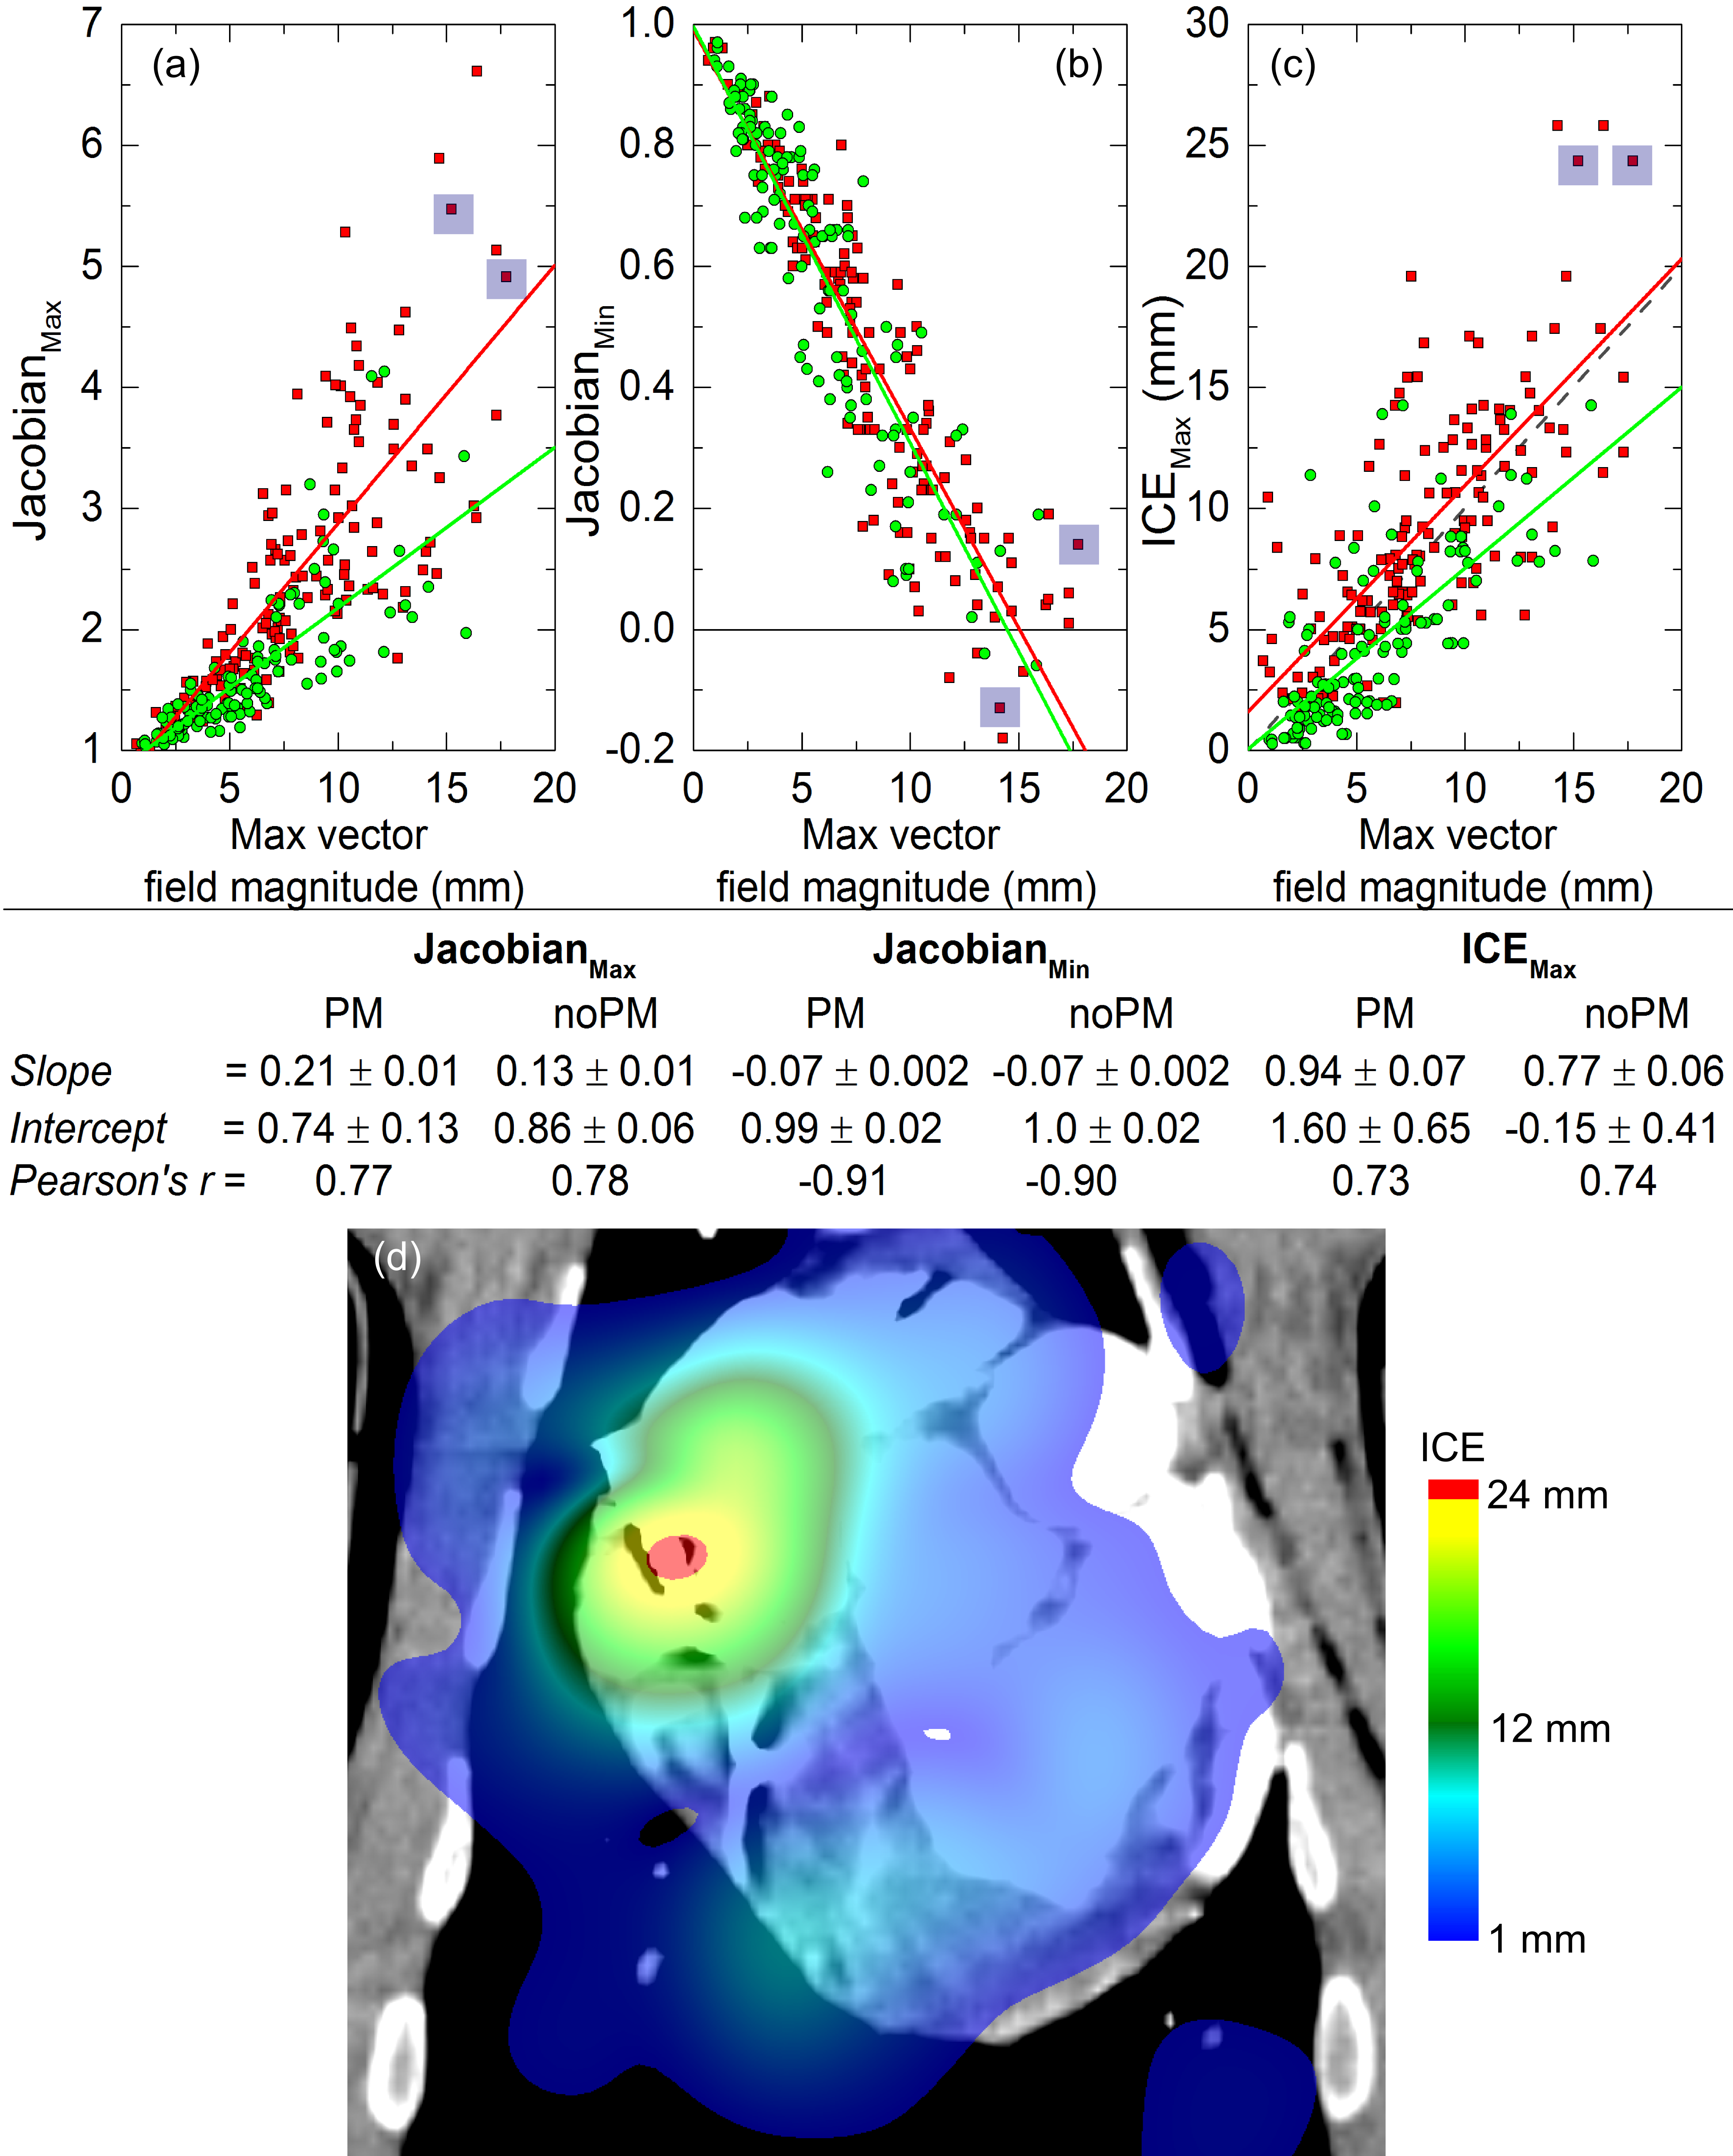
\includegraphics[width=0.9\textwidth]{./Vmm/Images/MaxVfdata_pigs.png}
		\caption{Values of maximum Jacobian (a), minimum Jacobian (b) and maximum ICE (c) plotted against maximum vector magnitudes. Linear fit is displayed with solid line and it's parameters are written below the plots. Dashed line in (c) shows $y(x)= x$ plot. Values from pig on image (d) are highlighted with blue squares in (a)-(c). PM and noPM are shown with red squares and green circles, respectively.
			ICE is displayed on (d) using the color table as displayed in the legend.}
		\label{maxvf_pigs}
	\end{center}
\end{figure}

\subsubsection{Discussion}

All 15 pig 4D-CTs have been registered, which resulted in 270 DIRs. DIRQA was performed in two steps - a smaller DIRQA during animal study on one state and a complete DIRQA on all 4D-CT states after it.

Mean vector field magnitudes were small (approx. 0.1 mm), since pigs were in a breath-hold position and the only motion was the heartbeat. 
Despite the small mean vector magnitudes it was still enough to observe statistical difference between the PM and noPM.
Consequently, the difference between the two groups is consistent throughout the DIRQA.

DIR did well in terms of lowering the absolute difference. There was a strong correlation between default versus true and inverse absolute difference. 
The slope of the linear fit on Fig.~\ref{absDiff_pigs} has the same value than the slope from lung 4D-CT (see Fig.~\ref{absDiff_lung}), showing
the effectiveness of B-Spline algorithm. The distribution of default absolute difference across different states is smaller than in lung 4D-CT (10 HU compared to 35 HU), due to the fact
there was less motion present in a pig 4D-CT. The shape of default absolute difference
distribution persist then in the Jacobian and ICE distributions as well. 

A good result in absolute difference does not necessary mean a good DIR, as can be seen from Jacobian and ICE checks. The mean Jacobian and ICE were 1 and 0, respectively, since the
vector fields were small on average. However there were large deviations present in Jacobian and ICE. Most notably, there were a few cases of negative minimum Jacobian which would suggest 
organ folding. Since organ folding did not occur during a heart beat, negative minimum Jacobian points to inconsistencies in DIR. 

The large deviations in Jacobian and ICE can in part be explained with large maximum vector field values, as shown in Fig.~\ref{maxvf_pigs}. All linear fits have a good correlation, with no
difference between PM and noPM in the quality of the fits. The actual linear fit parameters, however, further show the inconsistencies in DIR. The clearest example of inconsistencies in
DIR is with linear fit from maximum ICE PM, which lies above the function $y(x)=x$. This means that there were points further away from starting point after true and inverse transformation, 
then just after true transformation. The linear fit for noPM maximum ICE showed better results in this terms, since it lied below $y(x)=x$ function.


During the animal study only one DIR was repeated because of DIRQA. It was shown in post-experiment analysis, that all DIR should be repeated, pointing out flaws in initial DIRQA procedure.
Mainly, DIRQA should be made on all DIR and not just on one state, since DIRQA from one DIR does not guarantee the quality of the other DIRs from the same 4D-CT. 
Each DIR is performed individually and should be treated as such. Furthermore, instead of mean Jacobian and ICE, maximum and minimum should be investigated, 
because it points to the worst part of the DIR.



% \subsection{Mid-Position patient example}


\section{Summary and Discussion}
\label{Summary}

Tools to perform DIR and DIRQA have been presented in this chapter. Modules were written for an open-source software Slicer that can handle large DIR problems, such as registering whole 4D-CTs. 
In addition to DIR, the modules can also calculate DIRQA on DIR warped images and vector fields with several different checks.
The main objective of this work was to provide a systematic approach to DIR and to give parameters on DIRQA that can estimate the quality of DIR. A first analysis of DIRQA checks was done on a large DIR database - 684 DIR were checked in total.

Most of the work was based on Slicer, which is well-established software in medical research. To date, there are more than 500 publications that have used Slicer in their research \cite{SlicerCitation}, with topic ranging from 
teaching \cite{Pujol2016}, disease staging \cite{Liu2015, Liu2016b}, motion tracking \cite{Behringer2015} to image reconstruction \cite{Meyer2015}, image registration \cite{Li2015, Fedorov2015, Li2015b}
and others. Slicer offers ample functionalities and is especially suited for research, since it can be modified to specific needs. However, it is important to stress that Slicer 
is not a medical application. Additionally, Slicer can sometimes be unstable with unexpected crashes. It is constantly under development and more and more errors
are fixed with each new release. New releases also bring new functionalities, but there can be problems with backtrack compatibility. 
% Even though there are some disadvantages to using Slicer, it's advantages
% outweigh them and make Slicer a useful tool, as was shown in this chapter.

Results shown in this chapter were obtained with the B-Spline DIR algorithm. Several other algorithms exist, demons most commonly used alongside B-Spline \cite{Thirion1998}. Varadhan et al. compared B-Spline and demons DIR
for lung cases \cite{Varadhan2013} and showed that B-Spline is superior to demons, especially if there is difference in contrast between images. They used a mutual information
metric, to account for differences in contrast. Images used in this chapter were either all without (lung 4D-CTs) or all with (animal study 4D-CTs) contrast agent, therefore there was no difference in contrast
between images and mutual metric could not be used.
% . Mutual information metric was tested as well for DIR. For lung 4D-CT it could not complete DIR, because the states are too similar, however for the results were worse than mean square error metric. For lung 4D-CTs 

A designated module was written for DIRQA. The main advantage of the DIRQA module is that all different techniques are gathered in a single place and can be used on a specific case. 
The ease of use is also essential, for DIRQA to find its way into clinical work flow.
A test of using DIRQA in potential clinical work flow was done at GSI during the animal study, where different users operated with both DIR and DIRQA modules. The experiment was also under time pressure, since there was
a scheduled beam time. 4D-CTs were acquired approximately two weeks before the scheduled irradiation. During this two weeks contour delineation, DIR, DIRQA, treatment planing 
and treatment planning QA had to be done \cite{Lehmann2015}.
There were already propositions for frameworks for DIRQA in clinical work flow \cite{Varadhan2013}, however none were tested in an actual clinical environment. An animal study can not be directly compared to an actual clinic,
however the number of pigs studied was high (15) and the study was under time constraint, which simulate some of the pressures present in clinical environment.

The techniques used in DIRQA were divided into visual qualitative (inverse color, checkerboard) and quantitative (absolute difference, Jacobian and ICE). While the quantitative can be used to pinpoint errors in DIR, the visual qualitative
can be used to actually locate the error as shown in Fig.~\ref{maxvf}d. The location and size of DIR error also determines if a repetition of DIR is necessary.
All three quantitative checks have been used in literature as a possible DIRQA \cite{Varadhan2013, Leow2007, Christensen2001, Bender2009}.
They all share the same flaw, however, that they are a necessary but not sufficient condition for a successful DIR. 
One common DIRQA check in literature that our module is currently missing, is comparison of anatomical correspondence - 
comparison between reference, moving and warped contours. Ideally warped and reference contour should be the same. Two metrics are usually used in contour comparison -
dice similarity coefficient \cite{Varadhan2013} and Hausdorff distance \cite{Huttenlocher1993}. Slicer already has functionalities for both contour comparison checks, so they could be used. 
The biggest disadvantage of anatomical correspondence check is that contour delineation is required in both, reference and moving phase, which is scarcely done by physicians, 
since it takes too much time. Additionally, the anatomical correspondence check does not judge the vector field quality inside contour.
Lack of contours in both reference and moving phase was the reason the anatomical correspondence check was not used.

Studies on DIRQA so far have focused on a small number of DIR cases, whether it is phantom \cite{Mutic2001,Moore2004} or patient studies \cite{Wu2008, Varadhan2013}. With a small number of DIRs,
it is possible to thoroughly examine each DIR and hence understand DIRQA. In this work a different approach was
used. Rather than examining each DIR individually, a large dataset was analyzed and common traits for DIR were found. Due to differences in anatomical sites, 
DIRQA parameters have to be found for each anatomical site individually, since they can
deviate significantly, as seen by two different cases presented here. However, three checks are independent on anatomical site: mean true and absolute difference should be lower than 
default absolute difference, Jacobian should be positive and ICE should be smaller than maximum vector field magnitudes. 
If any of these checks fails, DIR needs to be investigated and, if necessary, repeated.
%However there may be parameters that persist throughout different anatomical sites, scaled Jacobian in particular.

DIR of lung 4D-CT can be considered relatively easy, since the contrast between lungs and other tissue is high. 
This is confirmed by a mean value of 1 for the Jacobian and mean ICE smaller than 1 mm. The maximum and minimum Jacobian and ICE are more interesting, since they show 
DIR inconsistencies. All ICE values bigger than maximum vector field magnitudes were found to originate from areas with poor DIR. An effect of poor DIR can be seen in Fig.~\ref{contourPropagation},
where propagated liver and lung contour do not match features on the image. An image artifact was the reason for the poor DIR. After investigation of poor DIR location and size, 
it was decided, that DIR does not require repetition, due to large distance between poor DIR and the tumor.
%This is supported by Fig.~\ref{calcJac_lung} and \ref{maxvf}. A small
%artifact was found in one phase and it was responsible for deviation from linear fit. Deviation from linear fit in Fig.~\ref{maxvf}a-c was also used to spot DIR inconsistencies
%and a lung image artifact was found in a different patient.

If the DIR of lung 4D-CT was considered relatively easy, opposite holds true for DIR of animal study 4D-CT. The motion of the heart during a heartbeat is complex, 
with muscles relaxing and contracting in different directions \cite{Seeley2007}. Furthermore,
the volume of blood shifts from one ventricle to the other. In the case of a cardiac 4D-CT, blood carried a contrast agent and blood distribution in heart was changing during a heartbeat. 
Therefore the HU distribution varied drastically in different cardiac 4D-CT states. Additionally, it is well established that pacemakers cause several complications in a CT scan \cite{Mak2012}. This was
confirmed by the differences observed between PM and noPM. Clearest example is the PM linear fit of maximum ICE in Fig.~\ref{maxvf_pigs}, which is above $y(x) = x$. For noPM the linear
fit is below $y(x)=x$, however the slope has still a value of 0.77, compared to 0.38 of a lung 4D-CT fit. Inconsistencies in DIR were further supported by negative minimum Jacobian, which were found for both,
PM and noPM groups. Negative minimum Jacobian and large ICE values are clear indicators, that DIR in heart can not be 
accepted for heart treatment planning and needs to be repeated. An effect of DIR on actual irradiation also has to be examined.
The DIR of cardiac 4D-CT is currently under careful investigation
and several different solutions, such as artifact removal and different registration parameters are being tested.

In the future, the DIRQA module should undergo further testing. In addition to checking DIRQA on different anatomical sites and between different modalities, 
it should be investigated how good is DIRQA at spotting inconsistencies in DIR, i.e. what is the number of false negatives. Furthermore, with more
data analyzed, the parameters in DIRQA checks should get more precise, so outliers could be more easily spotted.

Based on the findings presented here, several new features could improve the DIRQA module. Instead of mean, STD, maximum and minimum values, histograms could be displayed for quantitative tests.
Furthermore, histograms could be displayed for a specific contour, such as target, which would give a direct indication of DIR quality effect on treatment planning. 
Additionally, the module should automatically show the location of maximum and minimum Jacobian and maximum ICE.
The worst part of DIR would be hence immediately recognized and appropriate response could be formed.  
